% !TEX root = ../thesis.tex
\chapter{Experimenty}
\label{chap:experiments}

Jak již bylo zmíněno v předchozích sekcích, tak velmi významným problémem je psychologický faktor ztráty hlasu. To sebou nese i na první pohled neúplně zřejmý problém, kterým je obtížné získání získání řečníka po TL, který je ochotný spolupracovat na výzkumu.

Jedním z možných řešení je, že se výzkumníci sami naučí používat jednu z výše  \todo{TBD}{[c4l1]})zmíněných metod produkce řeči. Pro účely našeho výzkumu a rámec této práce by se jednalo o elektrolarynx. I když se tato možnost jeví poměrně jednoduše, tak zdání klame. Přestože je zdravý řečník schopen obstojně mluvit (pomocí EL), za relativně krátkou dobu tak k tomu, aby produkovaná řeč svými parametry odpovídala řečníkovi po TL, je potřeba relativně dlouhá doba.

Pro účely našeo výzkumu se nám podařilo získat pouze jednoho zkušeného řečníka\footnote{Jedná se o ženu v důchodovém věku, která ale stále působí na akademické půdě a jednou za čas i přednáší.}, který podstoupil TL před cca 15 lety a EL používá aktivně každý den. Je to jediná možnost jak produkovat slyšitelnou řeč.

Díky spolupráci s tímto řečníkem jsme byli schopni získat cca 15 hodin promluv (více o získaných datech v \ref{chap:experiments:analysis} a \ref{chap:experiments:normalization}), které byly použity pro všechny dosavadní experimenty. Z pohledu standardních obecných systémů rozpoznávání řeči se to může jevit jako velmi malé množství, ale jak ukáží následné experimenty, tak to není velký problém. Jelikož už před prvními experimenty se jevilo jako prozaičtější vytvářet individuální modely pro každého řečníka a výsledky experimentů toto jen podpořily.

Při rozhovorech s řečníkem se potvrdil psychický dopad ztráty hlasu na člověka po TL. Konkrétní osoba ještě dlouhá léta po operaci nebyla schopna telefonovat natož mluvit na veřejnosti. Kvalita života se tímto velmi snížila a trvalo prý velmi dlouho dobu, než se daná osoba odvážila i jen odpovědět na nečekaný telefonní hovor.

V následujícím textu si přiblížime a zanalyzujeme pořízená data (\ref{chap:experiments:analysis}), dále popíšeme důvody normalizace dat a porovnáme schopnosti člověka a stroje (\ref{chap:experiments:normalization}). V sekci \ref{chap:experiments:poc} rozebereme prvotní ověřovací experimenty s upravenámi daty a v sekci \ref{chap:experiments:durationmodels} představíme výsledky modelů zohledňujících i délku fónému.

% Při konzultacích s pacienty vyšlo najevo, že psychická stránka je velmi důležitá a někdy to může věst až k paralýze (v obrazném slova smyslu) kdy ti lidé nebyli schopni třeba telefonovat. Takže systém, který by sice neřešil kompletní problematiku náhrady/rehabilitace řeči by mohl být užitečný.

% !TEX root = ../thesis.tex
\section{Analýza dat a první modely}
\label{chap:experiments:analysis}

Rozpoznávání řeči se věnuje nemalé usílí již od 50. let 2O. století a v současné době nikoho nepřekvapí téměř bezchybně fungující obecný rozpoznávač v mobilních zařízeních. Pro obecné systémy dokonce existují korpusy s desítkami či stovkami a více hodin promluv, které je možné využít při vytváření těchto systémů.

Tyto korpusy však obsahují ve většině případů pouze \uv{standardní}\footnote{Slovením spojením \uv{standardní řeč} je myšlena řeč neobsahující vyrazné řečové vady, případně jiné formy produkce a často v nepřílíš akusticky náročném prostředí.} řeč. Pokud je snaha vytvořit nebo ověřit funkčnost systému za specifických podmínek (ať už se jedná o rušné prostředí či speciální typy promluv), tak je nezbytné získat potřebná data.

\subsection{Vytvoření korpusu EL promluv}
\label{chap:experiments:analysis:corpus}

Na začátku byla idea o pomoci skupině lidí mající problémy s přirozenou řečí. Vůbec prvním předpokladem, na cestě k úspěšnému dosažení vůbec nějakého cíle, jsou data. Jelikož se jedná o velmi spefická data, tak je potřeba zajistit co možná největší množství kvalitních\footnote{Kvalitou je myšlena věrnost dat dané doméně, dále se mluví o přesnosti ve smyslu bezchybnosti přepisů.} a přesných dat.

V části \ref{sec:cause:desease} bylo zmíněno, že ročně se objevý více než 100 nových případů trvalé ztrázy hlasu ročně. Zaroveň bylo řečeno \cite{Skvrnakova2010}, že více rizikovými osobami jsou starší lidé, kteří intenzivně kouří a konzumují alkohol. Přesto je patrný trend snižujícího se věku pacientů a s tím souvisejícím nárůstem případů ztráty hlasu. Přičteme-li již zmíněný psychologický aspekt jeho ztráty, tak je zřejmé, jak komplikované je získat ke spolupráci i jen jednoho řečníka ochotného podstoupit naročné\footnote{I pro zdravého člověka je někdy někalikahodinové nahrávání vysilující. Pro jedince po TL to je z mnoha důvodů ještě řádově náročnější.} nahrávání.

Při libovolné práci s pacienty po TL, dřív nebo později dojde k určité formě spolupráce s oddělením ORL, které má nastarosti péči o tyto pacienty. V našem připadě nejprve s ORL klinikou při Fakultní nemocnici v Plzni a poté i s ORL klinikou Fakultní nemocnice v Motole. S jejich pomocí jsme získali ke spolupráci jednoho řečníka. Konkrétně se jedná o dámu v duchodovém věku, která podstoupila TL před více než 15 lety. Po překonání ostychu\footnote{Podle jejích vlastních slov nebyla schopna několik let po operaci ani zvednout nečekaný telefonní hovor, natož mluvit na veřejnosti.} se byla schopna naplno vrátit do běžného života a dokonce v určité formě opět přednášet o stomatologii na Lekařské fakultě v Plzni Univerzity Karlovy.

S její pomocí jsem, v 1. etapě nahrávání, byli schopni pořídit přes 10 hodin promluv, viz tab. \ref{tab:experiments:analysis:recording}. Nahrávání probíhala v relativně spartánských podmínkách za plného běžného provozu katedry. Přesto získaná data neosahují žádný nežadoucí ruch, kromě toho produkovaného samotným EL.

Nahravací aparatůra sestávala z miniaturního profesionálního mikrofonu (DPA d:screet 4061-FM), zesilovačem (DPA MMA6000), externí zvukovou kartou a běžného notebooku. Mikrofon byl pomocí bezpolštářkové náplasti přilepen poblíž pravého koutku úst, abychom zaznamenaná řeč měla co možná nejvyšší kvalitu.

Celé nahrávání bylo v 1. etapě rozděleno do 14 samostatných sezení a probíhalo od prosince roku 2010 do května roku 2011. Každé sezení trvalo přibližně dvě hodiny během kterých se podařilo získat necelou hodinu akustických dat. Samotné nahrávání se sestávalo z 10 - 20 minutového úseku pořizování nahrávky a přibližně 10 minut dlouhého odpočinku. Ten byl nezbytný hlavně z důvodu únavy řečníka.

Ještě před samotným nahrávánám byly pečlivě vybrány a vytvořeny 2 sady vět:

\begin{enumerate}
  \item sada obsahující všechny možné české fonémy - \textit{40 vět}.
  \item sada obsahující věty s reálnou četností fonémů - \textit{5000 vět} \cite{Radova2000}.
\end{enumerate}

\noindent Pořízené nahrávky vždy odpovídají 10 - 20 minutovému úseku nepřerušovaného nahrávání a soubory tak vždy obsahují několik vět. Ty jsou od sebe odděleny minimálně 5 sekundovým úsekem ticha. Nahrávky dále mouhou obsahovat opakování chybně vyslovené věty, přeřeknutí, kýchnutí a další neřečové události. Z tohoto důvodu bylo nezbytné pořízené nahrávky anotovat, přestože byly pořízené na základě připravené sady vět.

Ještě před samotným anotováním byly nahrávky, podle úseků s tichem, rozsekány na menší části. V tomto případě úplně dobře nefungovali\footnote{Problémem byl zvuk EL, se kterým nebylo při návrhu VAD počítáno.} standardně používané sofistikovanější metody pro voice activity detection (angl. zkratka VAD), a proto bylo využito principu energie. Pro každou nahrávku obsahující více vět se pomocí vzorce

\begin{equation}
  \label{eq:experiments:analysis:energy}
  E_{RMS}(n) = \sqrt{\frac{1}{N} \sum_{n=1}^{N} \left| x(n) \right|^2},
\end{equation}

\noindent kde $N$ představuje počet vzorků v nahrávce a $x(n)$ představuje pravoúhlé okénko vzorku $n$. Pro tento případ se ukázalo jako vhodnější volit root-mean-square energy ($E_{RMS}$) a empericky se ukázalo, že vhodná délka okénka je v rozmezí $10 - 100$ ms. Na obr. \ref{fig:experiments:analysis:el_speech} je zobrazena podoba audio signálu a spektrogram promluvy \textit{\uv{Akcie Komerční banky}}. Zároveň je zde vypočtené hodnoty energie a celková průměrná energie. Tyto hodntoty slouží pro určení míst kde začíná a končí věta. Na začátku a konci každé věty je dobré mít minimálně $0.5$ s ticha. Tím pádem, pokud energie nějakého úseku $x$ je $E_{RMS}(x) < avg(E_{RMS})$ a zároveň délka tohoto úseku $dur(x) \geq 1\ [s]$, tak nahrávku můžeme v tomto úseku rozdělit.

\begin{figure}[hbpt]
  \centering
  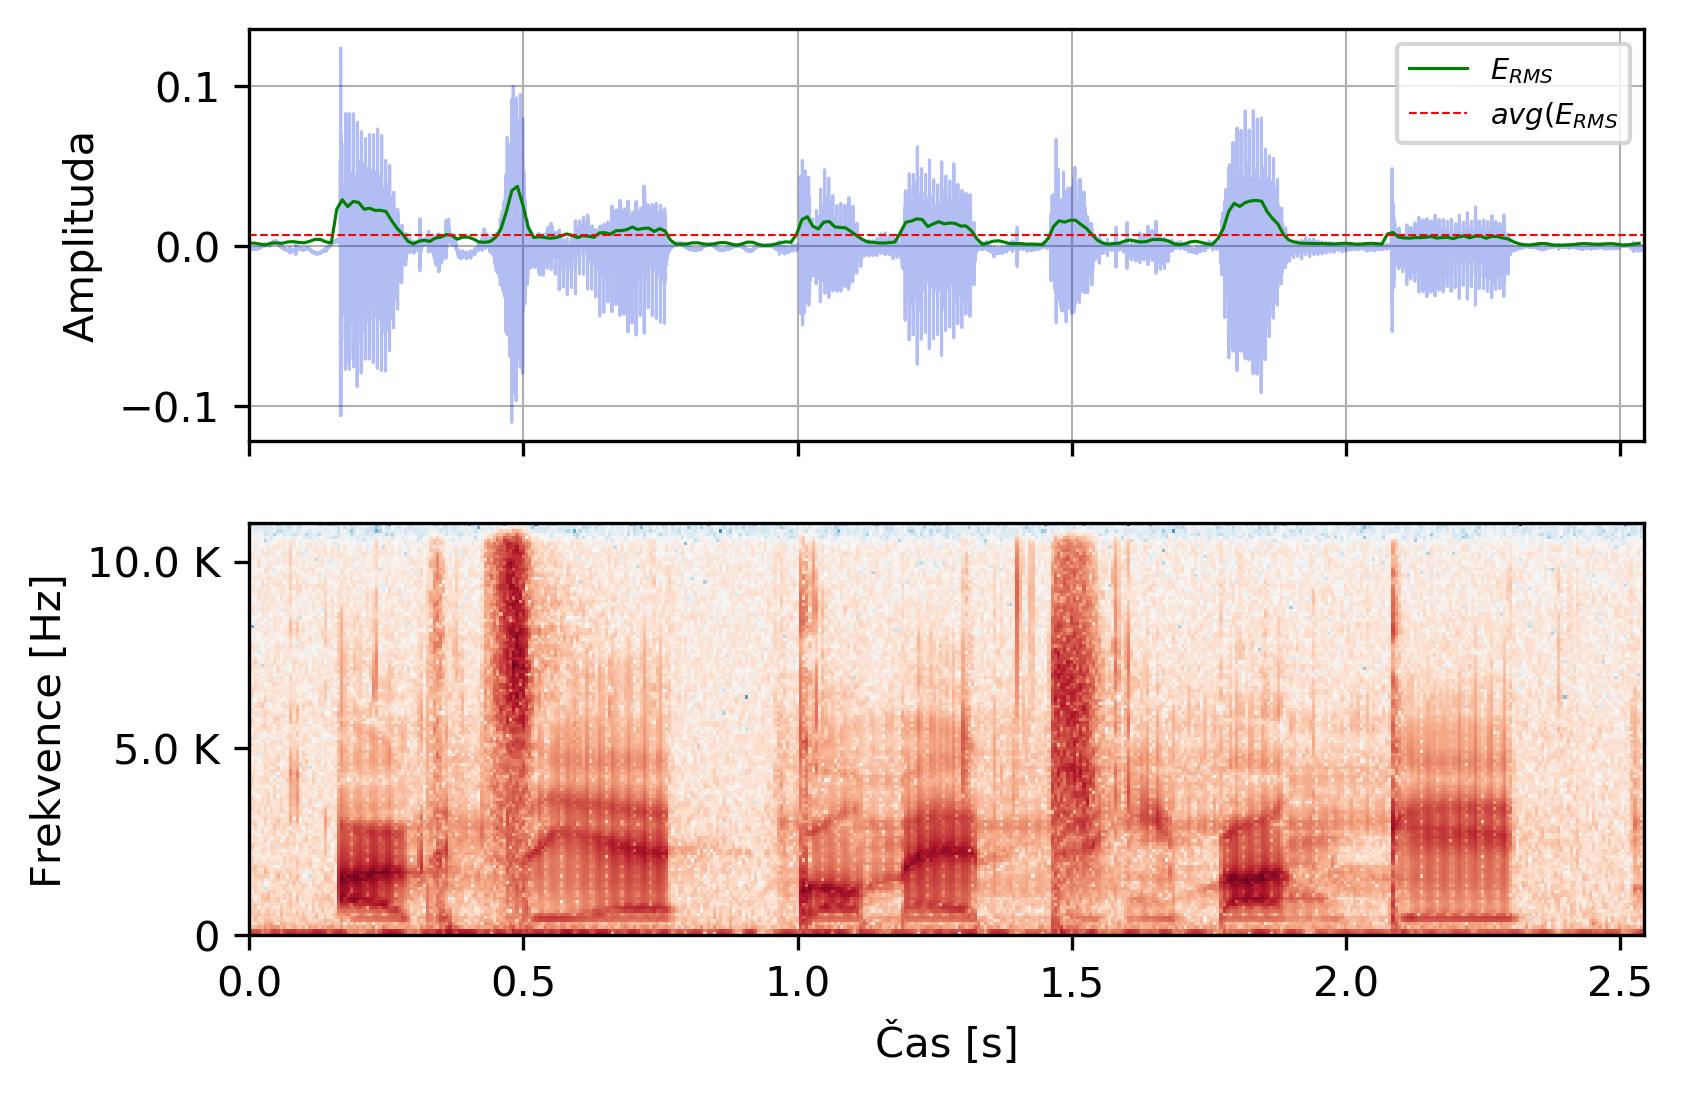
\includegraphics[width=0.9\textwidth]{./ch4-experiments/img/energy_spec_el.png}
  \caption{Průběh a spektrogram promluvy a vyznačenou energií EL promluvy.}
  \label{fig:experiments:analysis:el_speech}
\end{figure}

Samozřejmě pokud řečník v průbehu věty z libovolného důvodu udělal větší pauzu než $1$ s, tak tato věta byla rozdělena. Jelikož jsou výsledné kratší useky promluv následně anotovány, tak to nepředstavuje problém. Pro budoucí zpracování není podstatné zda promluva je opravdu celá věta, ale to jestli je tento úsek správně přepsán. Fakt, že některé věty jsou rozděleny je důvodem proč v tab. \ref{tab:experiments:analysis:recording} více souborů než vět.

K anotaci posloužil interní nástroj určený k tomuto účelu a podíleli se na něm celkem 3 anotátoři z řad studentů, kteří si vzájemně kontrolovali své anotace. Ačkoli bylo potřeba anotovat relativně malé množství dat (cca 10 hodin audio záznamu), tak anotace zabrala přibližně 2 měsice. Hlavním důvodem byla relativně dlouhá doba, po kterou se anotátoři adaptovali na specificka EL řeči. Problémem bylo to, že nejprve nebyli vůbec schopni poruzumnět obsahu promluvy a tím pádem jej správně přepsat.

Pokud je pro produkci řeči použit elektrolarynx, tak vedlejším produktem je nezanedbatelný ruch způsobený samotným zařízením \ref{sub:cause:treatment:foniatric}. Přeci jen jeho jedinout funkcí je vybudit vzduch v dutině ústní a tím umožnit produkci slyšitelné řeči. Z tohoto důvodu byly v průběhu anotace ignorovány v podstatě všechny skupiny neřečových událostí, protože vetšinu obsahu nahrávek by bylo nezbytné anotovat jako, že obsahují šum.

Výsledný korpus tedy představuje $5040$ unikátních vět rozdělených do $6385$ souborů (viz tab. \ref{tab:experiments:analysis:recording}), které v průměru obsahují $7$ slov o průmerné délce $5$ znaků. Tento korpus slouží jako základ pro všechny budoucí experimenty.

\begin{table}[htpb]
  \centering
  \def\arraystretch{1.5}
  \pgfplotstabletypeset[
    col sep=comma,
    string type,
    columns/phase/.style={column name=Nahrávání, column type={|l}},
    columns/length/.style={column name=Délka \textit{[HH:MM:SS]}, column type={|r}},
    columns/sentences/.style={column name=Počet vět, column type={|r}},
    columns/files/.style={column name=Počet souborů, column type={|r|}},
    every head row/.style={after row=\hline, before row=\hline},
    every last row/.style={after row=\hline},
  ]{./ch4-experiments/tabs/02-recording1-stats.csv}
  \caption{Informace o korpusu nahrávek z 1. etapy nahravání.}
  \label{tab:experiments:analysis:recording}
\end{table}

\subsection{Analýza získaných dat}
\label{chap:experiments:analysis:data}

Po dokončení anotace obsahuje korpus přes 10 hodin akustických záznamů promluv a více či méně přesných přepisů\footnote{I přes nemalou snahu a několikastupňovou kontrolu, je téměř jisté, že by nebylo obtížné najít přepis, který obsahuje chybu například ve formě překlepu.}. Když jsou k dispozici data je možné se podívat na specifika EL řeči a případně porovnat se zdravým řečníkem.

Pro potřeby porovnání byl použit začátek promluvy \textit{\uv{Akcie Komerční banky...}}. Tuta promluva je součástí standardní množiny vět používaných při vytváření řečových korpusů na KKY při ZČU. Tím pádem je k dispozici v relativně velkém množství příkladů pro zdravé řečníky a také je součástí korpusu EL řeči.

Na obr. \ref{fig:experiments:analysis:el_speech} a \ref{fig:experiments:analysis:normal_speech} je zobrazen průběh signálu a spektrogram vybrané promluvy. Už na první pohled je možné zaznamenat určité rozdíly. Prvním takovým je délka promluvy, v případě zdravého řečníka je o celou 1 vteřinu kratší než v případě EL řeči. Tempo řeči je samozřejmě velmi individuální, ale z principu je EL řeč pomalejší. Z průbehu signálu na obr. \ref{fig:experiments:analysis:el_speech} je patrné, že řečník dělá výraznější pauzy mezi jednotlivými slovy promluvy. To může být způsobené například potřebou naplnit jícen vzduchem. Po TL je dýchání realizováno přes tracheu a pokud nebyl voperován shunt (více v \ref{sub:cause:treatment:tracheo}), tak je trvale oddělen hrtan a hltan. Přesto, pro produkci některých neznělých fonémů je potřeba exhalovat vzduch z dutiny ústní. Zkušený EL řečník to dělá naprosto automaticky, nicméně \uv{polykání} vzduchu zabere nějaký čas. Nevyhnutelným důsledkem je pak velmi častý výskyt samovolného říhání v průběhu promluvy\footnote{Fakt, že je říhání jako neřečová událost běžnou součástí téměř každé promluvy, vedl k ignorování těchto událostí během anotace.}.

\begin{figure}[hbpt]
  \centering
  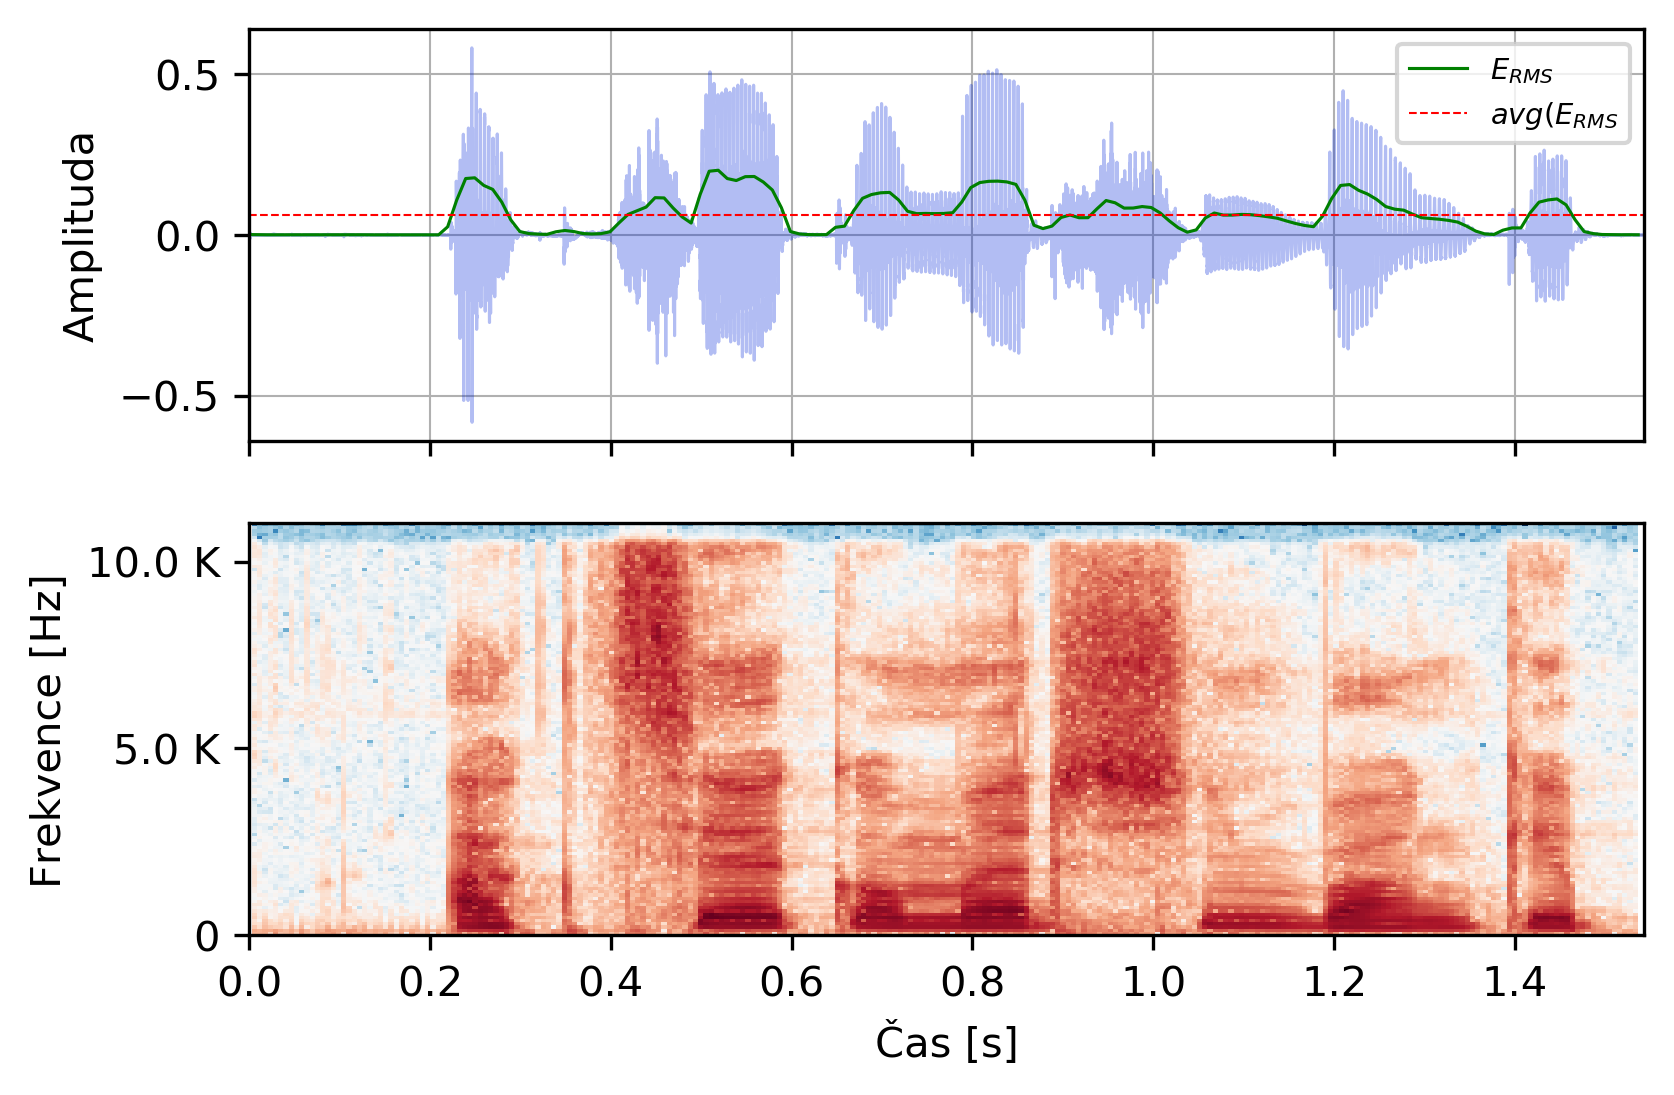
\includegraphics[width=0.9\textwidth]{./ch4-experiments/img/energy_spec_normal.png}
  \caption{Průběh a spektrogram promluvy a vyznačenou energií promluvy.}
  \label{fig:experiments:analysis:normal_speech}
\end{figure}

Dalším důvodem může být je nutnost správné artikulace. Při používání EL je to nezbytné, aby bylo produkované řeči alespoň trochu dobře rozumnět. A pokud se dobře artikuluje, tak není snadné mluvit rychle. Při nahrávání bylo také velmmi běžné, že v průběhu promluvy řečník udělal pauzu, aby mohl lépe umístit EL, protože jeho umístění má velký vliv na kvalitu produkované řeči. Nicméně je třeba říci, že tempo není a priory pro ASR systémy problém, protože různá délka fonémů je v relativně snadno modelována, např. v HMM přechodem ze stavu do stejného stavu.

Dalším způsobem jak ukázat rozdíly mezi promluvou zdravého řečníka a řečníka s EL je srovnání ve frekvenční oblasti. Pro větší názornost jsou na obr. \ref{fig:experiments:analysis:spectrogram} vedle sebe zobrazeno spektrum ukázková promluva zdravého řečníka (\ref{fig:experiments:analysis:spectrogram:normal}) a toho s EL (\ref{fig:experiments:analysis:spectrogram:el}). Obsah obou promluv je identický a přesto jsou obě spektra odlišná.

Prvním markantním rozdílem je mnohem větší zastoupení šumu v úsecích \uv{ticha} na obr. \ref{fig:experiments:analysis:spectrogram:el}. To je nepochyně způsobnemo samotným EL, který řečník nevypíná mezi jednotlivými slovy. Na obr. \ref{fig:experiments:analysis:el_speech} je to také zřetelně patrný, zejména na průběhu energie, šum zejména před prvním a druhým slovem promluvy. Zajímavá je přítomnost šumu v célém frekvenčním spektru, přestože EL produkuje konstantní buzení. Toto buzení je ve spektru, na obr. \ref{fig:experiments:analysis:spectrogram:el}, viditelná jako výrazná souvislá linie v nízkých frekvencích. Přitomnost šumu ve vyšších frekvencích je způsobena umístěním mikrofonu, který je nalepen na pokožku a tím pádem snímá namodulované vibrace, přenášené měkkou tkání. Tento fakt se potvrdil v dalších etapách nahrávání (viz \todo{přidat zmínku o tom, že v dalších etapách to je krapet jinak}{porovnání}), kde byl použit studiový mikrofon vzdálený od úst minimálně 15 cm. Nicméně z pohledu použitelnosti nějakého budoucího systému je nezbytné počítat i se situací, kdy mikrofon bude zaznamenávat i vibrace přenášené tkání.

Dalším markantním rozdílem je absence vyšších frekvencí u většiny produkovaných fonémů. Vyjímku tvoří afrikáty $/c/$ a $/\check{c}/$, u kterých jsou hlasivky (u zdravého jedince) v klidu a vznikají uvolněním nahromaděného vzduchu v dutině ústní\footnote{Nahromadění vzduchu je realizováno přitisknutím jazyka k přední/zadní části horního patra.} \cite{Psutka2006}. V tomto případě není, u řečníka po TL, principiálně tento mechanizmus produkce těchto fonému ovlivněn. Problémem teoreticky může být zdroj vzduchu, jelikož jej z plic není možné dostat do dutiny ústní, ale jak už bylo zmíněno (a spektrogram to potvrzuje) zkušený uživatel EL se dokáže adaptovat.

Absence vyšších frekcencí se dá vysvětlit použitím EL, kde samotný EL má vždy konstantní frekvenci buzení a dále tím, že nedochází k modulaci v ve všech dutinách vokálního traktu. Nicméně nejdůležitější složky, zajišťující srozumitelnost, se vyskytují ve frekvenčním pásmu od 1 kHz do 3 kHz. Vyšší frekvence se a priory podílejí na zabarvení hlasu.

\begin{figure}[htpb]
  \centering
  \begin{subfigure}[b]{0.4\textwidth}
    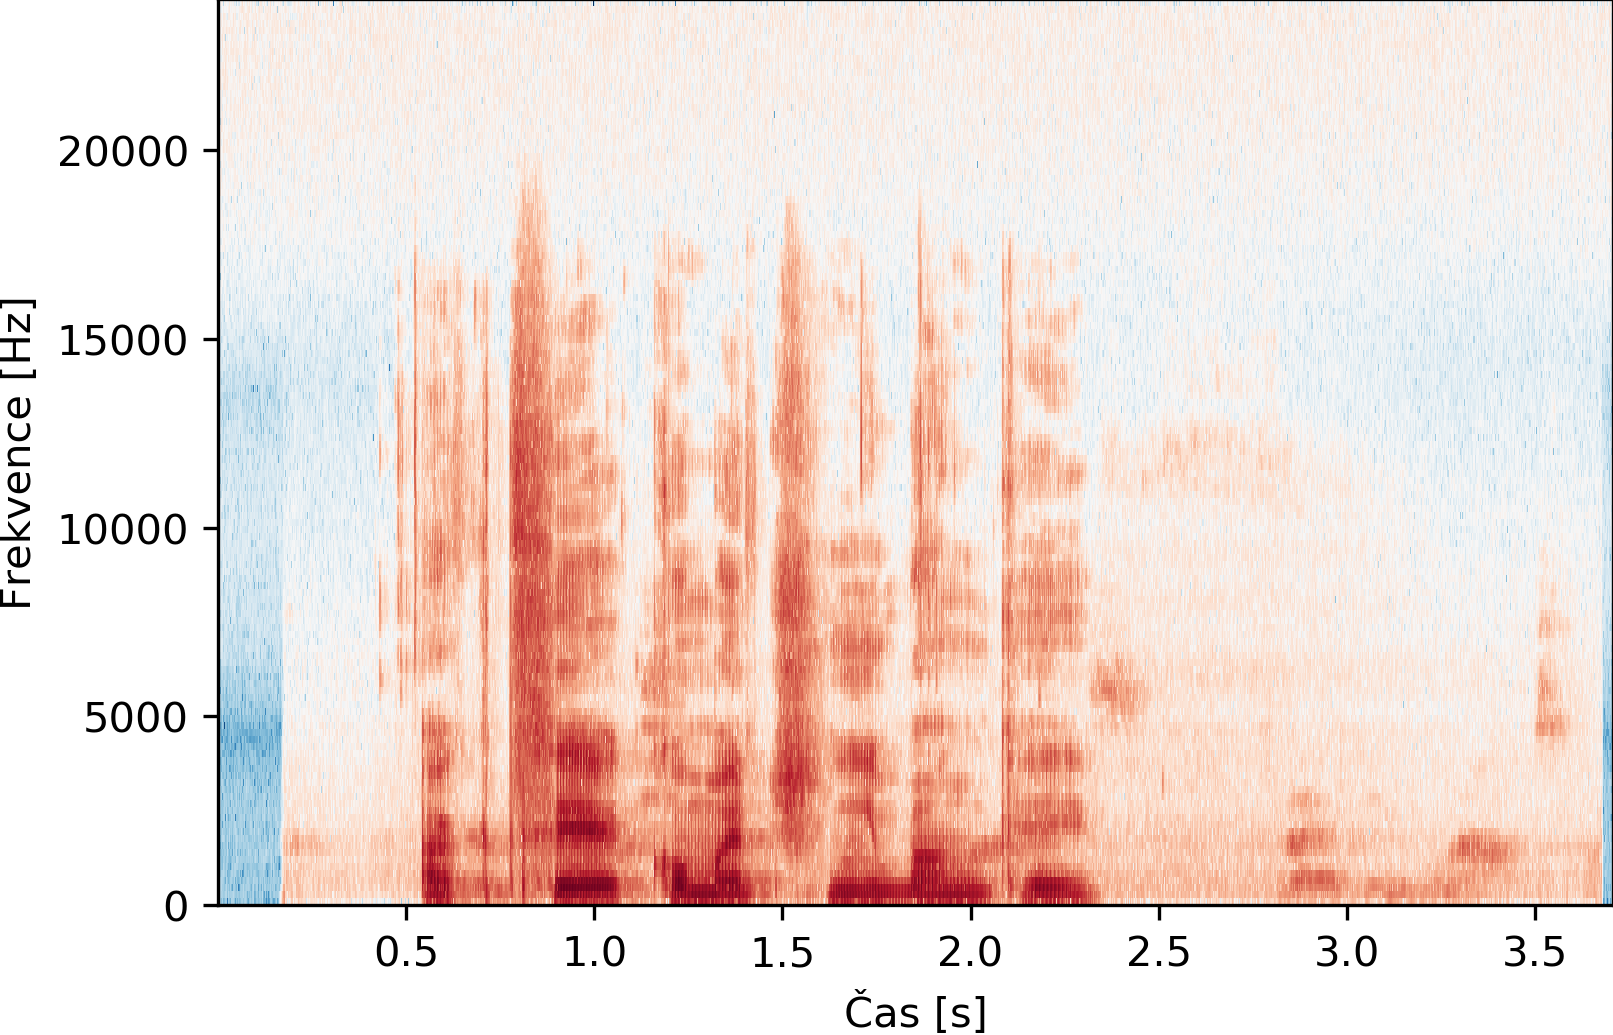
\includegraphics[width=\textwidth]{./ch4-experiments/img/spectrogram_normal.png}
    \caption{Zdravý řečník}
    \label{fig:experiments:analysis:spectrogram:normal}
  \end{subfigure}
  %
  \begin{subfigure}[b]{0.4\textwidth}
    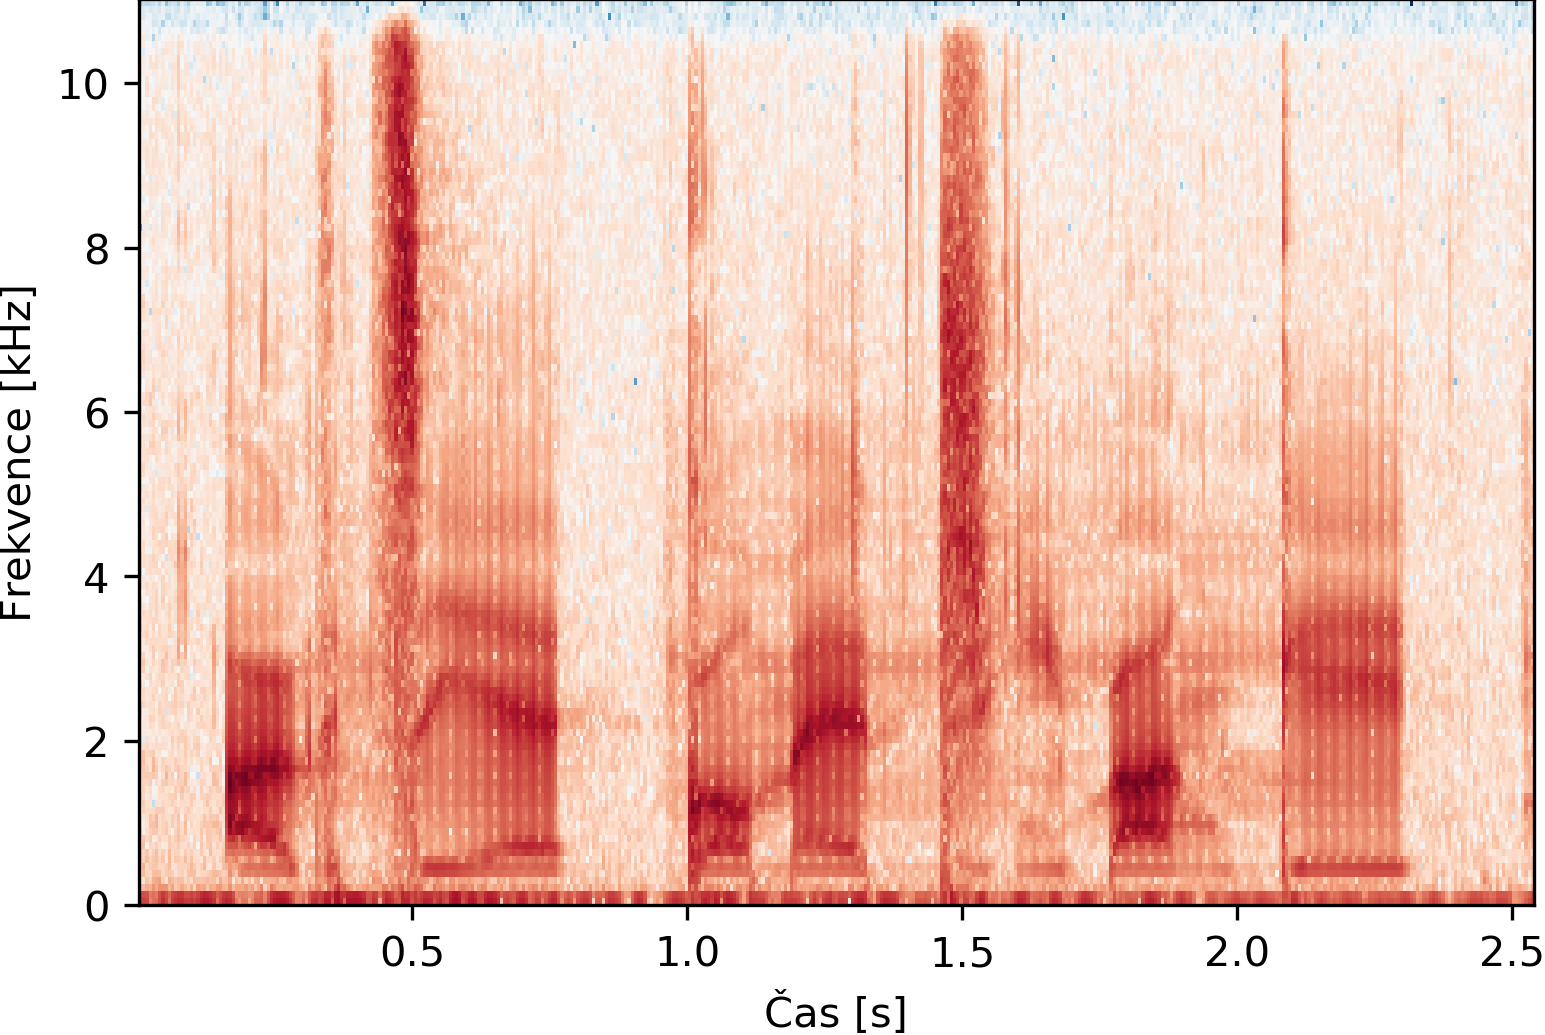
\includegraphics[width=\textwidth]{./ch4-experiments/img/spectrogram_el.png}
    \caption{EL řečník}
    \label{fig:experiments:analysis:spectrogram:el}
  \end{subfigure}
  \caption{Spektrogram promluvy \uv{Akcie Komerční banky} dvou řečníků.}
  \label{fig:experiments:analysis:spectrogram}
\end{figure}

Dalším způsobem jak porovnat řeč zdravého řečníka a tím s EL je pomocí analýzy jednotlivých fonémů. Na obr. \ref{fig:experiments:analysis:phonemes} jsou zobrazeny průběhy amplitudy v čase\footnote{Hodnoty času, na obr. \ref{fig:experiments:analysis:phonemes}, odpovídají časům výskytu v původní promluvě.} pro fonémy $/k/$, $/m/$ a $/\check{c}/$. V případě $/k/$ a $/m/$ (1. a 2. průběh) se jedná o okluzivy, kde v prvním případě se jedná o neznělou plozivu a druhém o znělou plozivu. Tyto fonémy obecně vznikají uzavřením vydechovaného proudu vzduchu, pomocí artikulačních orgánů, což se projeví jako krátká pauza (tzv. okluze). Po té následuje náhlé jednorázové překážky a únik nahromaděného vzduchu, tzv. exploze \cite{Psutka2006}. Takto popsáno to samozřejmě funguje u zdravého jedince, ale u EL řečníka jde principiálně o stejný mechanizmus. S tím rozdílem, že vzduch nepochází z plic, ale z hltanu. Dalším rozdílem je samozřejmě absence hlasivek.

\begin{figure}[htpb]
  \centering
  \begin{subfigure}[b]{0.42\textwidth}
    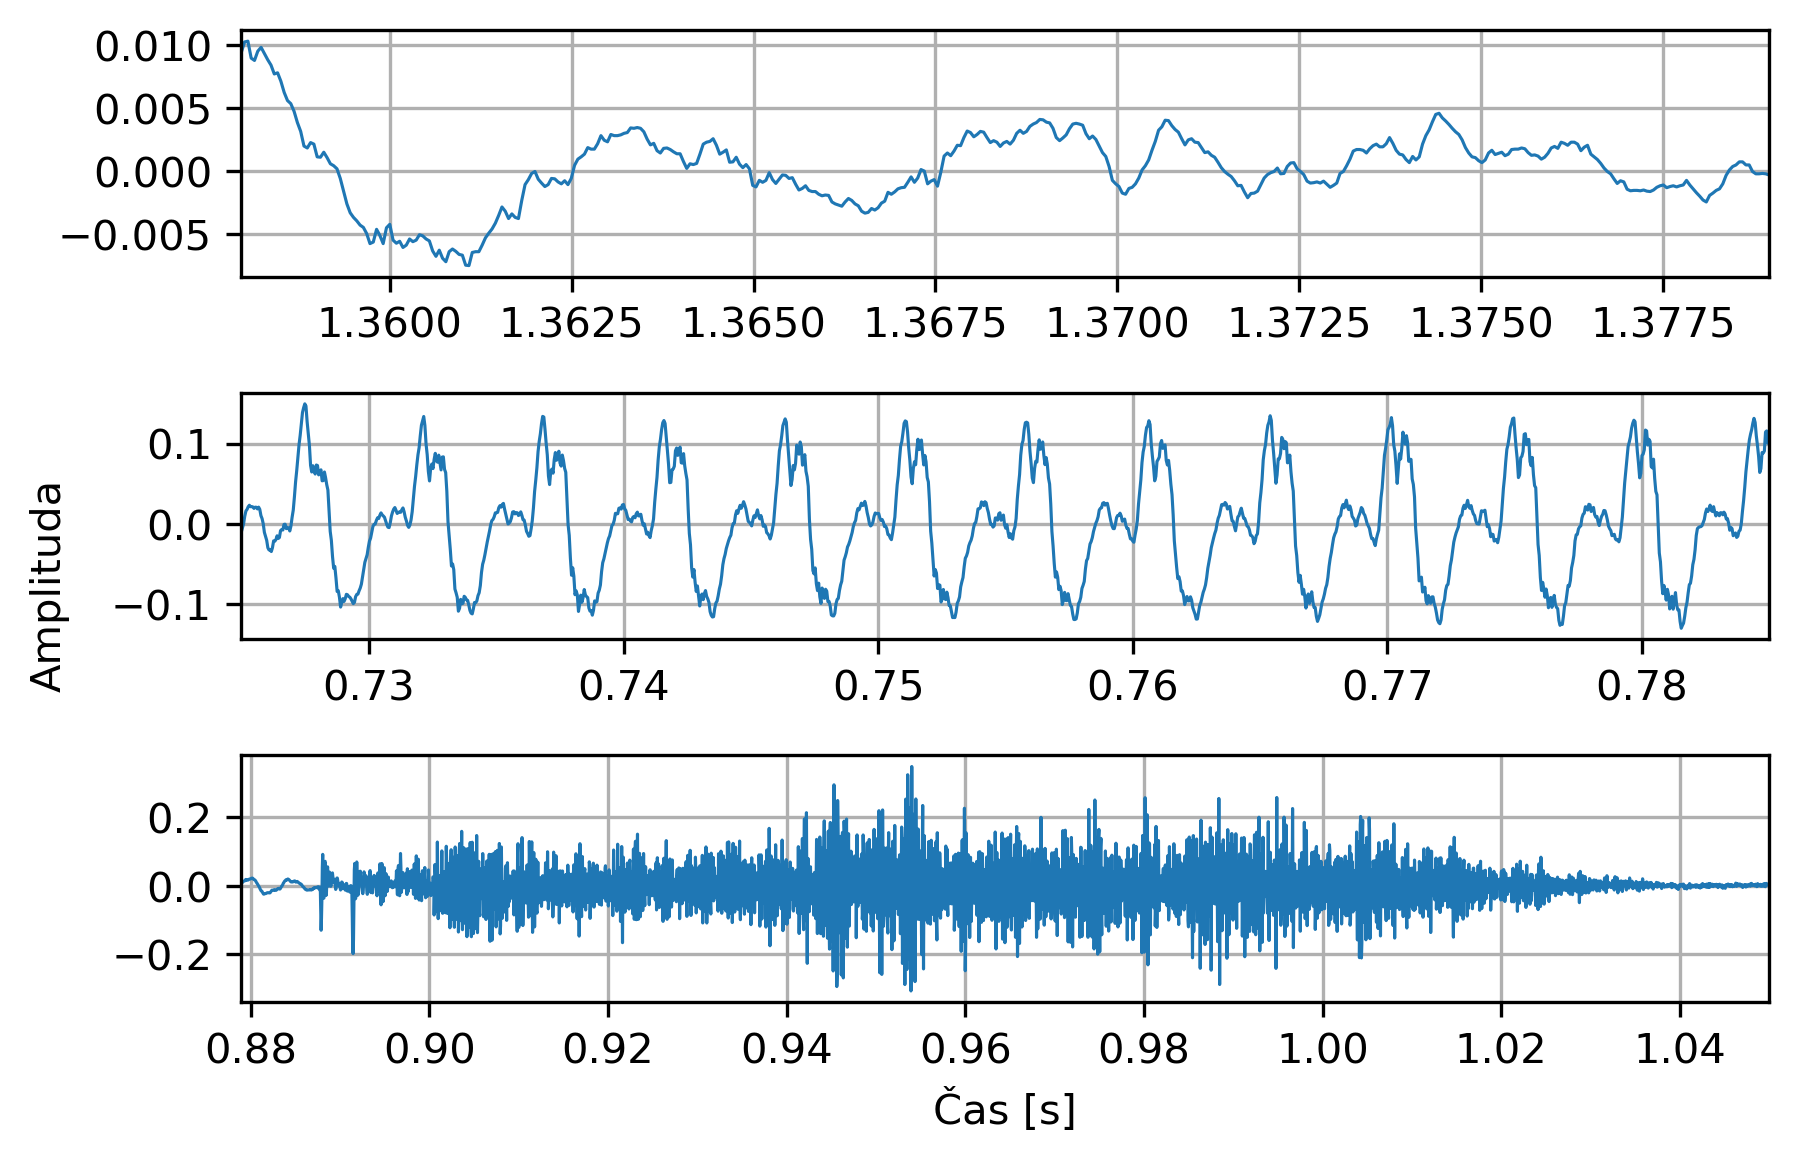
\includegraphics[width=\textwidth]{./ch4-experiments/img/phonemes_normal.png}
    \caption{Zdravý řečník}
    \label{fig:experiments:analysis:phonemes:normal}
  \end{subfigure}
  %
  \begin{subfigure}[b]{0.42\textwidth}
    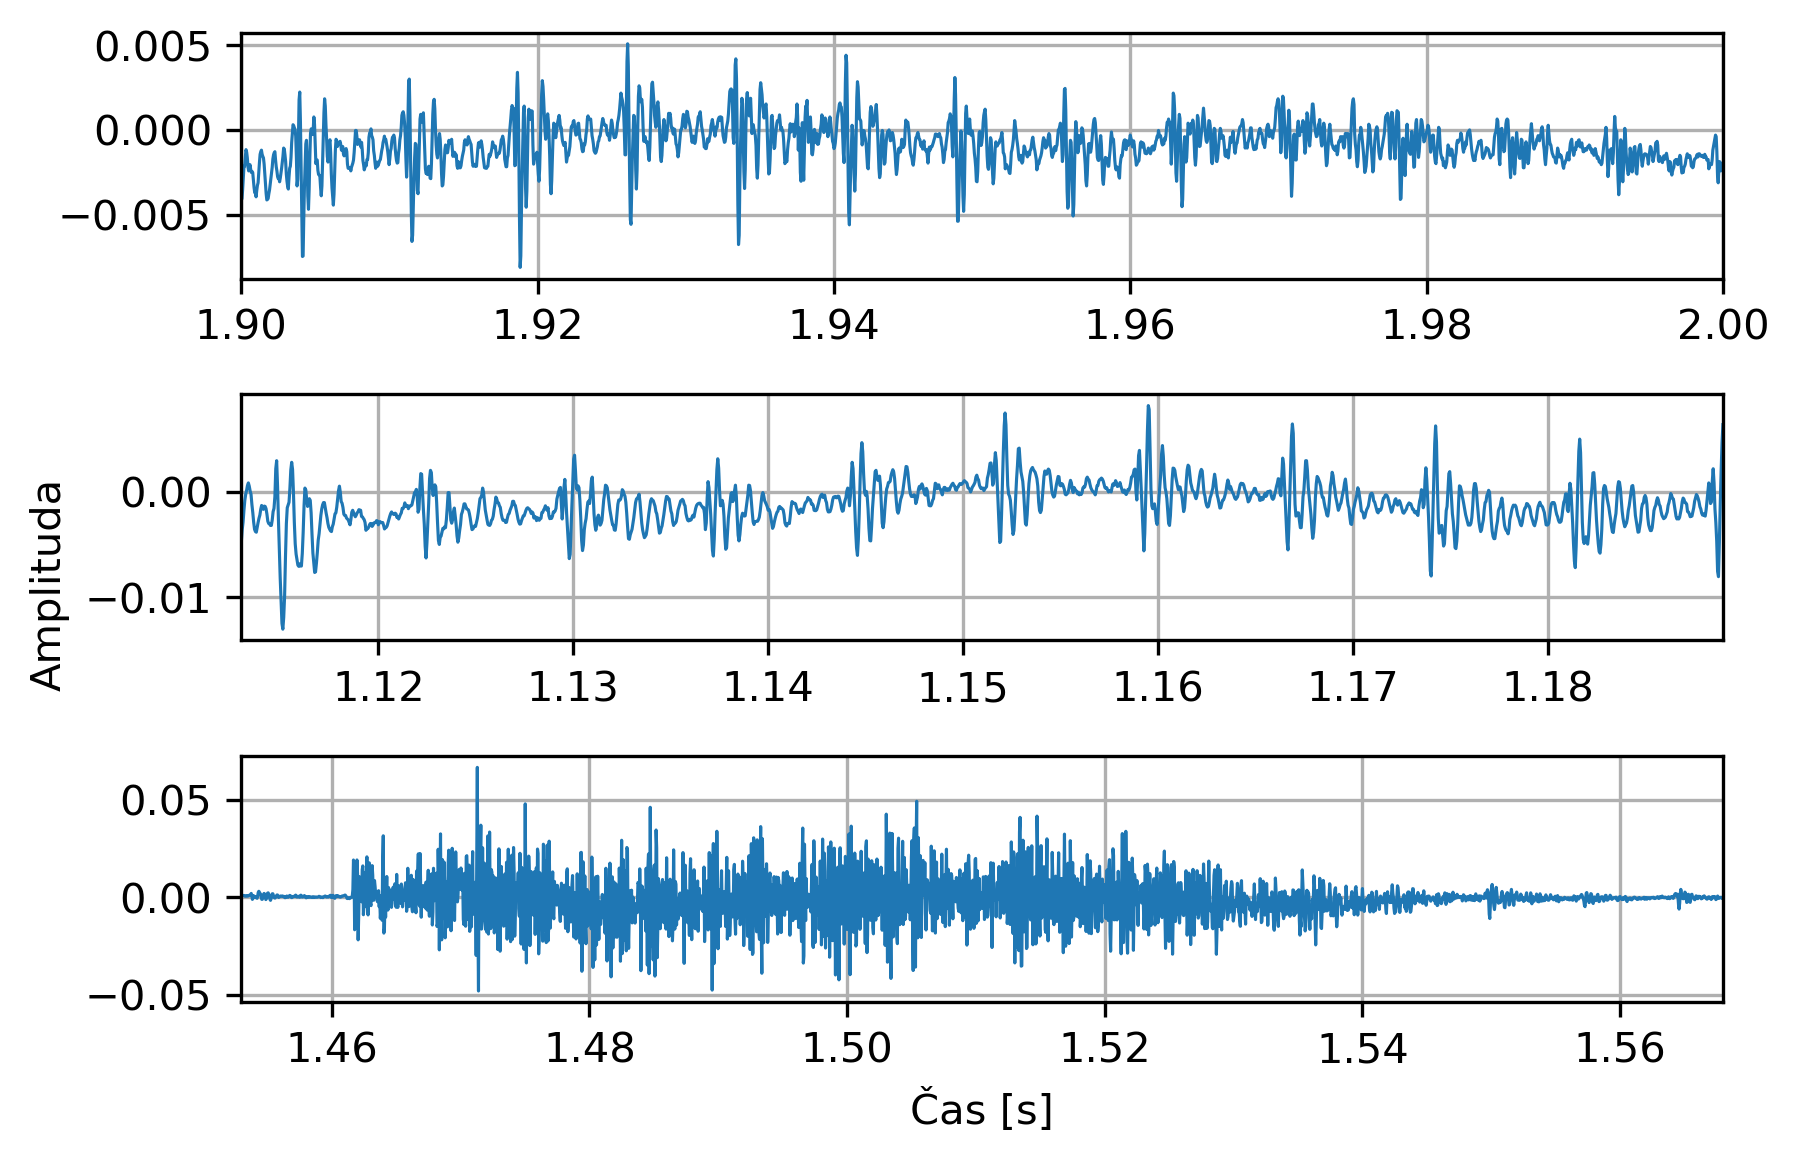
\includegraphics[width=\textwidth]{./ch4-experiments/img/phonemes_el.png}
    \caption{EL řečník}
    \label{fig:experiments:analysis:phonemes:el}
  \end{subfigure}
  \caption{Ukázky průběhů amplitudy pro fonémy $/k/$, $/m/$ a $/\check{c}/$.}
  \label{fig:experiments:analysis:phonemes}
\end{figure}

Foném $/k/$ představuje zástupce neznělých fonémů, ty se vyznačují tím, že do jejich produkce nezasahují hlasivky, které jsou v klidu. Zdrojem buzení je tedy šum. Pokud se podíváme na průběh amplitudy v čase u zdravého řečníka (obr. \ref{fig:experiments:analysis:phonemes:normal}), tak zde není vidět žádný periodický signál. Hlasivky jsou tedy opravdu v klidu. Oproti tomu u EL řečníka (obr. \ref{fig:experiments:analysis:phonemes:el}) je jasně patrné, že je zde přítomno aktivní buzení vytvořené EL. Na obr. \ref{fig:experiments:analysis:freq:k} je pak zobrazeno tzv. amplitudové spektrum, které znázorňuje vývoj amplitudy signálu ve frekcenci pro oba řečníky. V případě zdravého řečníka odpovídá vývoj očekávání tedy, že zde není žádná výrazná frekvence a také, že nedochází k výraznému útlumu. Přestože se v obou případech jedná o stejný foném, tak z časového i frekvešního průběhu amplitudy je zřejmé, že parametry signálu se u obou řečníku diametrálně liší.

\begin{figure}[hbpt]
  \centering
  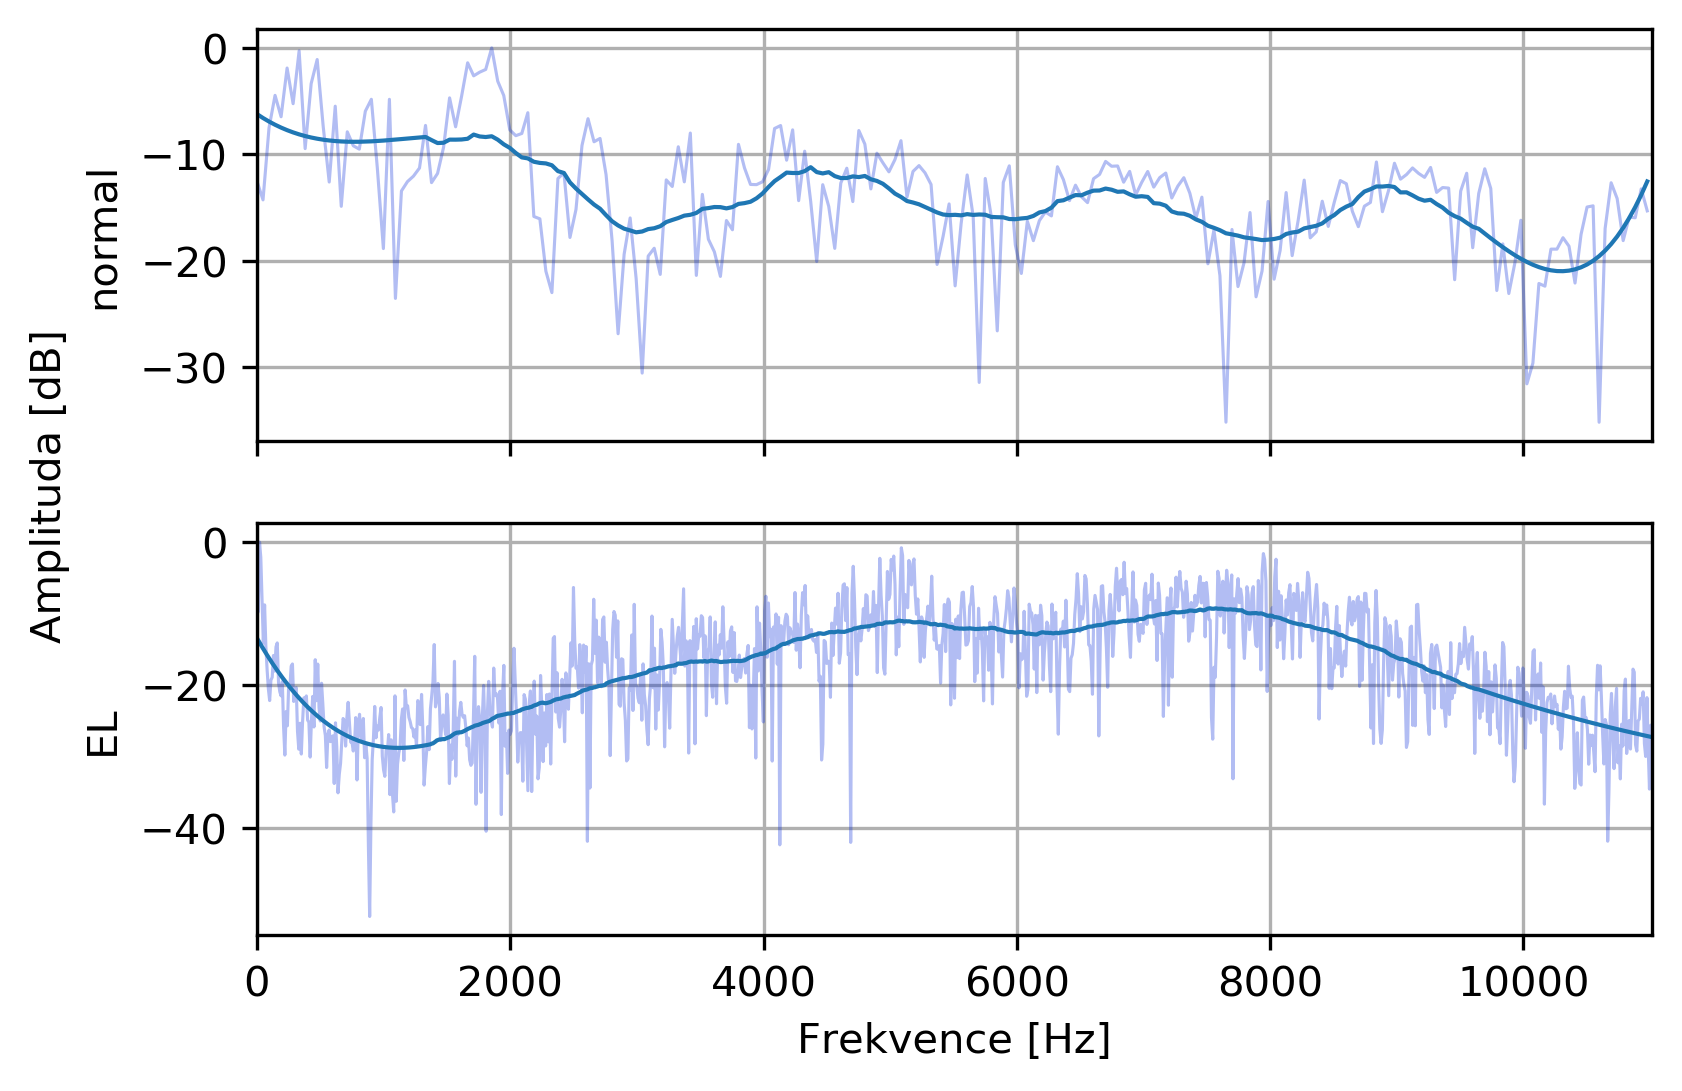
\includegraphics[width=0.9\textwidth]{./ch4-experiments/img/freq_analysis_(k).png}
  \caption{Vývoj amplitudy fonému $/k/$ ve frekvenci zdravého (horní) a EL (dolní) řečníka.}
  \label{fig:experiments:analysis:freq:k}
\end{figure}

Jako druhý ukázkový foném slouží $/m/$. Opět se jedná o plozivu, ale v tomto případě o znělou. U těchto fonémů hrají velký vliv hlasivky, protože jsou zdrojem buzení. Z obr. \ref{fig:experiments:analysis:phonemes:normal} je krásně zřetelné buzení ve formě perodického průběhu amplitudy. Narozdíl tomu, u EL řečníka (obr. \ref{fig:experiments:analysis:phonemes:el}) je také vidět periodický signál, ale úplně jiného průběhu. Svým způsoběm dost podobný tomu, který je zřetelný u fonému $/k/$. Rozdíl je zřetelný i ve frekvenční oblasti (obr. \ref{fig:experiments:analysis:freq:m}), kdy u EL řečnía nedochází útlumu ve střední oblasti frekvenčního spektra.

\begin{figure}[hbpt]
  \centering
  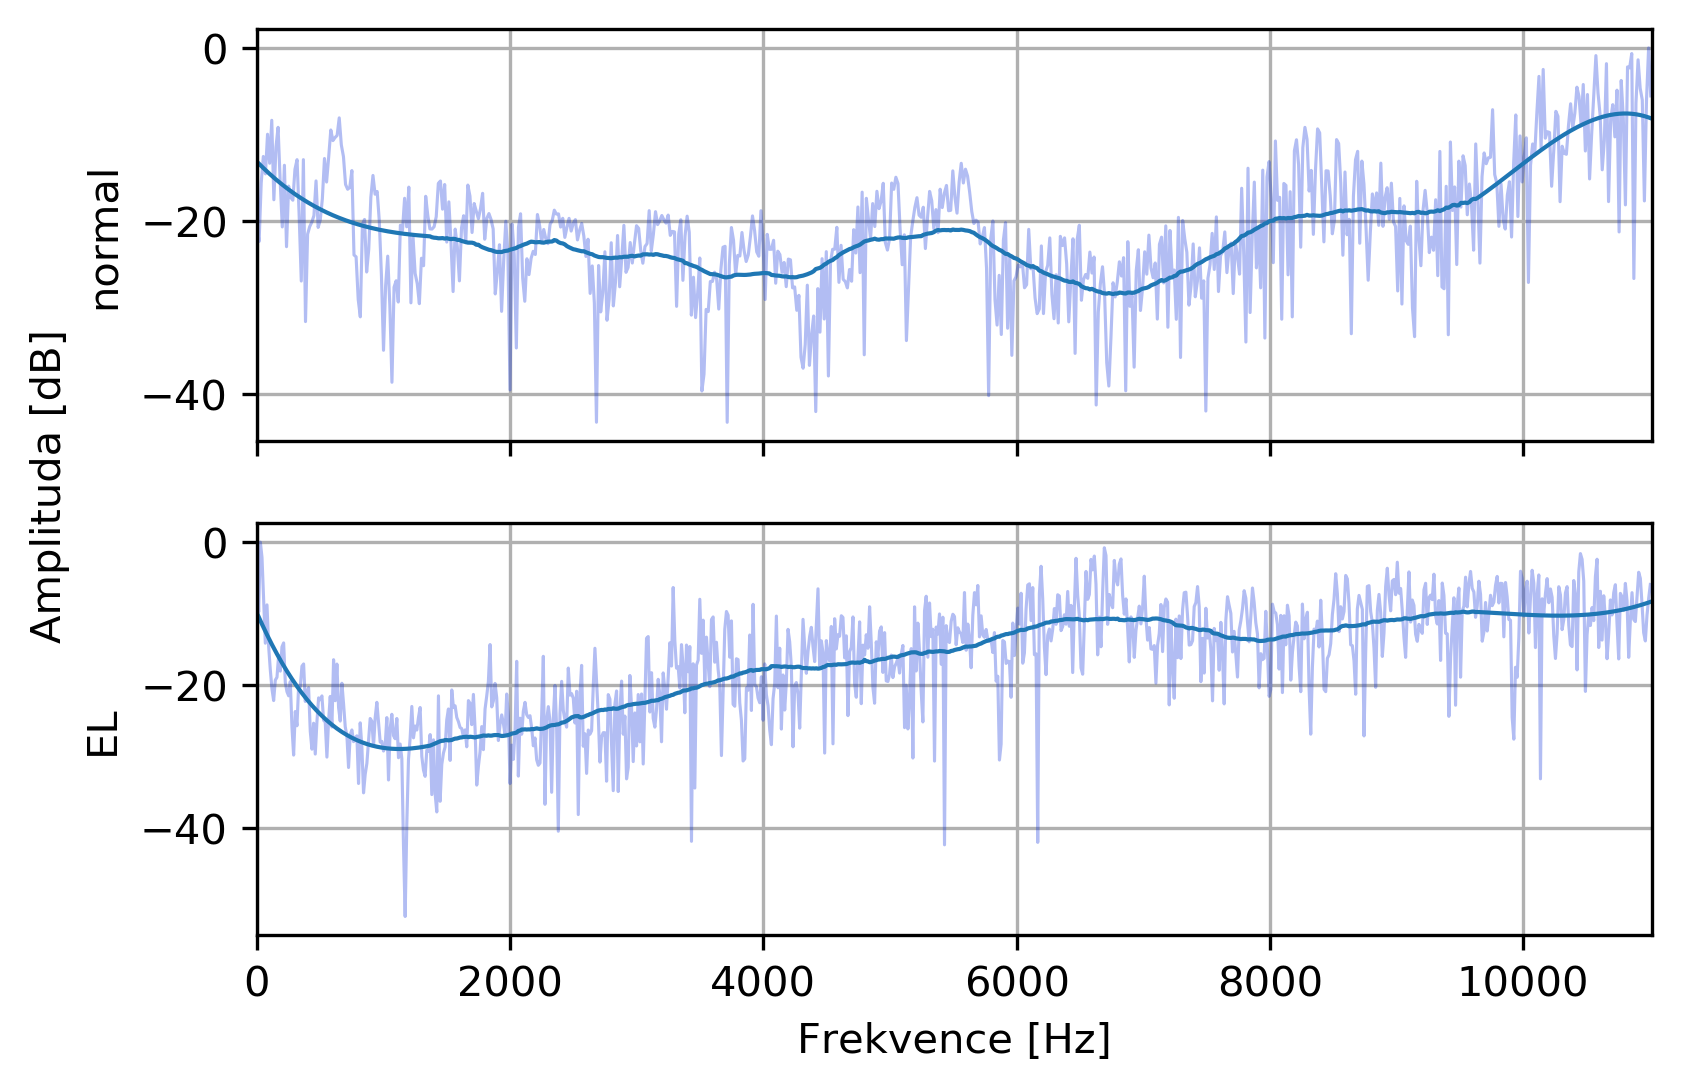
\includegraphics[width=0.9\textwidth]{./ch4-experiments/img/freq_analysis_(m).png}
  \caption{Vývoj amplitudy fonému $/m/$ ve frekvenci zdravého (horní) a EL (dolní) řečníka.}
  \label{fig:experiments:analysis:freq:m}
\end{figure}

Posledním úkázkovým fonémem je již zmiňované $/\check{c}/$. Jedná se o neznělý foném, který vzniká přiložením jazyku k zadní části horního patra. Tím je zadržen vzduch v dutině ústní a vzniká krátká pauza. Uvolněním pak dochází k explozi a vytvoření zvuku. Do produkce se nezapojují hlasivky a produkovaný zvuk by měl být dostatečně intenzivní, aby jej (v případě EL řečníka) tolik neovlivňoval EL. Tím pádem by měl být průběh signálu, u obou řečníků podobný, a to jak v časové, tak i ve frekvenční oblasti. Na obr. \ref{fig:experiments:analysis:phonemes} a \ref{fig:experiments:analysis:freq:c} je pak jasně vidět, že se jedná o platný předpoklad.

\begin{figure}[hbpt]
  \centering
  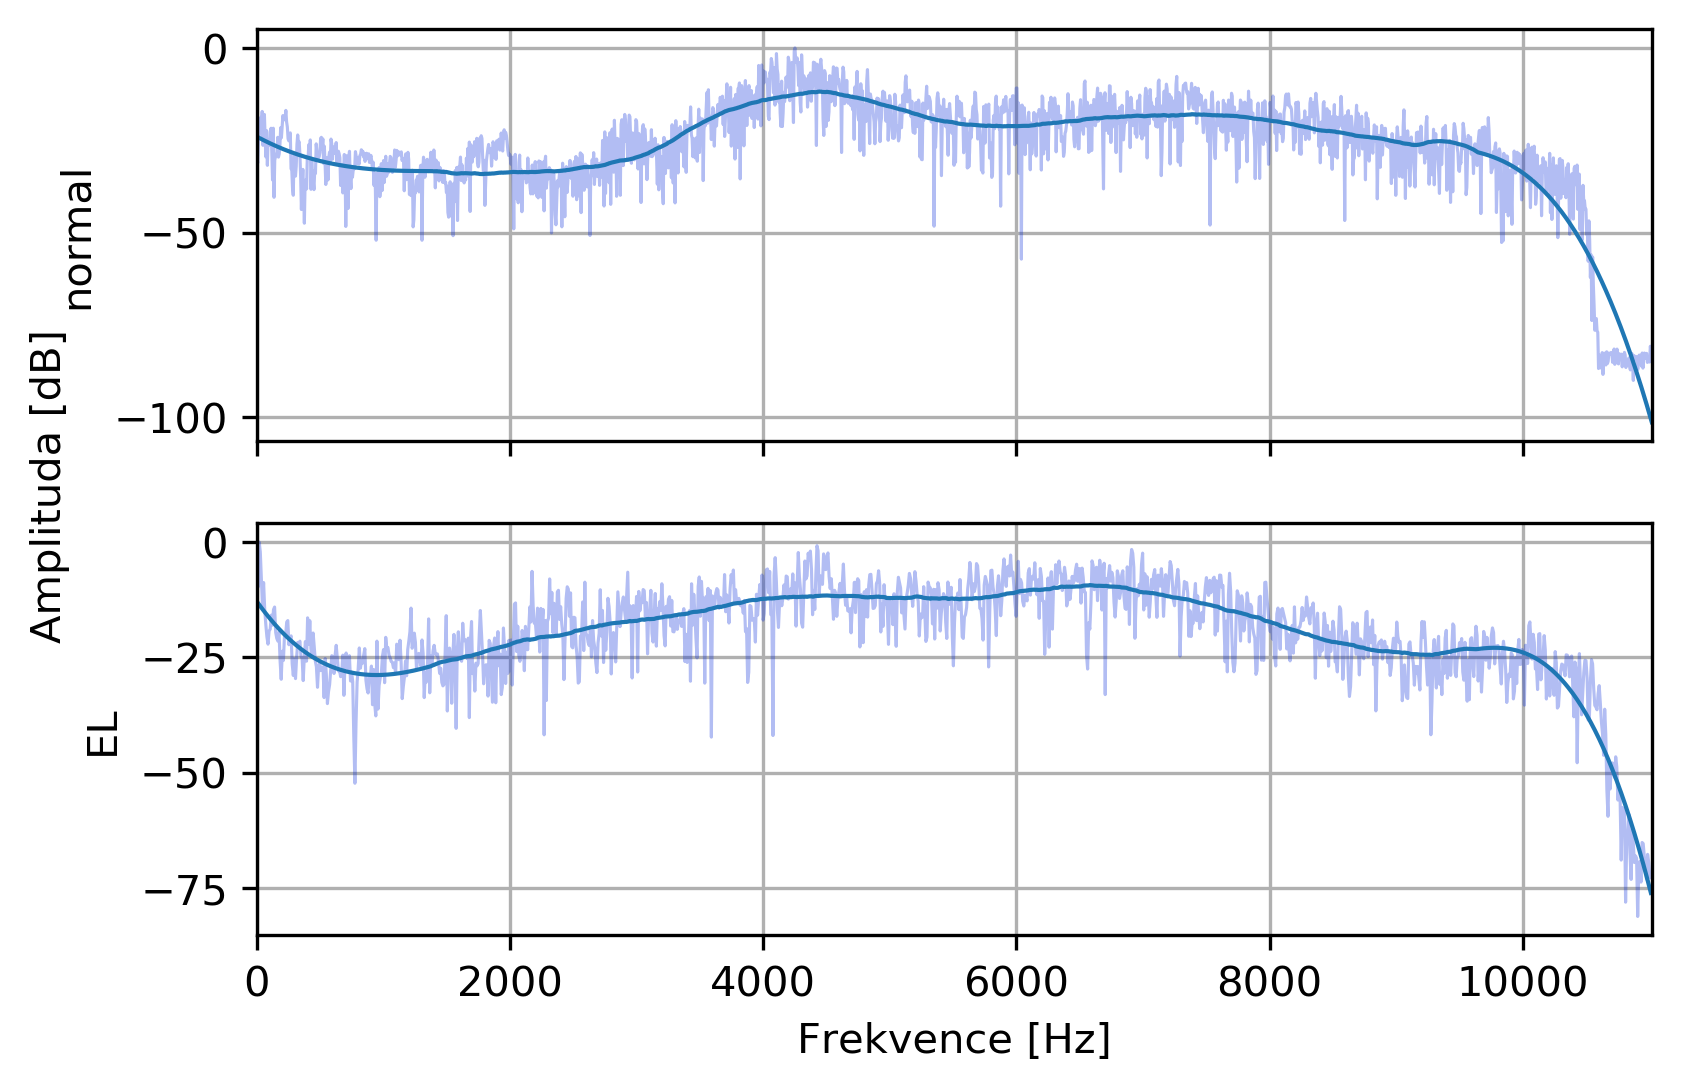
\includegraphics[width=0.9\textwidth]{./ch4-experiments/img/freq_analysis_(c).png}
  \caption{Vývoj amplitudy fonému $/\check{c}/$ ve frekvenci zdravého (horní) a EL (dolní) řečníka.}
  \label{fig:experiments:analysis:freq:c}
\end{figure}

Z doposud provedené analýzy plyne, že EL řeč je v mnoha charakteristikách odlišná od té produkované zdravým řečníkem. Zejména u porovnání ve frekvenční oblasti (obr. \ref{fig:experiments:analysis:freq:k} a \ref{fig:experiments:analysis:freq:m}) je to nejvíce patrné. Tento fakt nepochyně přispívá k tomu, že standardní obecné modely rozpoznávání řeči nedosahují takové přesnosti jako v případě bežné promluvy.

% \csvautotabular{./ch4-experiments/test.csv}

\subsection{Prvotní experimenty}
\label{chap:experiments:analysis:experiment}

Z výsledků \textbf{TBD} je patrné, že EL doména je diametrálně odlišná od bežné řeči, pro které jsou ASR systémy vytvářeny. Navíc, pokud se vezme v potaz náročnost získání potřebných dat pro natrénování obecného modelu, tak se jako jediná schůdná varianta jeví vytváření individuálních modelů pro každého řečníka. To znamená, že model je trénovaný pouze z dat odpovídající konkreténímu řečníkovi a často i účelu použití. K vytvoření takového modelu je zapotřebí řádově méně dat, při dosažení podobného výkonu. Stinnou stránkou je případná menší robustnost modelu. Čistě logicky tento model bude fungovat pouze s konkrétním řečníkem a ještě jen v situacích, které odpovídají trénovacím datům. U řečníků s EL může navíc hrát velký vliv samotný EL. Již při nahrávání se ukázalo, že jeho pozice může nepříznivě ovlivnit kvalitu řeči. Tento problém by však neměl významně ovlivňovat kvalitu modelu, protože tento fenomém je obsažen v datech. Co se však ukázalo jako potencionálně problematické, je stabilita parametrů produkované řeči v dlouhodobém časovém úseku. Více o tomto problému pak v části \textbf{TBD}. K zodpovězení nejdůležitější otázky, jestli takový model vůbec může fungovat, stačí získaná data z první etapy nahrávání a ta obsahují řeč s relativně konzistentními parametry.

V rámci ověřování funkčnosti infividuálního modelu je vhodné zkusit různé varianty, aby se určili optimální parametry modelu. Hlavními uvažovanými hyperparametry je vzorkovací frekvence audio nahrávek a počet HMM stavů. Originální pořízené nahrávky mají vzorkovací frekvenci rovnu $44,1 kHz$, pro úlohu rozpoznávání je to zbytečně moc, protože nejvíce informace je obsažena ve frekvenčním pásmu do $4 kHz$, vyšší frekcence a priory ovlivňují zabarvení hlasu apod. \cite{Psutka2006} Otázkou je jestli stačí vzorkovací frekvence rovna $8 kHz$ nebo lépe $16 kHz$, kde je přeci jen více informací. Počet stavý modelu pak ovliňuje množsví modelovaných trifónů. Čím více stavů, tím více je modelovaných trifónů. Stinnou stránkou pak je fakt, že čím více stavů, tím více  je potřeba trénovacích dat. Množina uvažovaných možností obsahuje $1024,\ 2048$ a $4096$ stavů. Jen pro vysvětlení je dobré zmínit, že HMM stav představuje model jedné uvažované akustické jednotky (nebo skupiny jednotek s podobnými parametry). Počet stavů nám tedy říká, kolik takových jednotek model dokáže rozlišit. Čím více stavů, tím více jednotek (menších skupin) je modelováno. Teoreticky tak model s více stavy je lepší. Nicméně k natrénování jednotky je potřeba určité množství dat a tím pádem je pro model s vyšším počtem stavů logicky potřeba větší množství trénovacích dat. Samozřejmě fonetická sada neobsahuje $4096$ fonémů, neobsahuje ani $1024$ fonémů\footnote{Ve skutečnosti obsahuje 42 českých fonémů.}. U těchto modelů se pak používá nějaký druh \textit{n-gramové} reprezentace fonémů, nejčastěji pak trifóny.

Celkově je tak natrénováno $6$ modelů. K natrénování akustických modelů je použit HTK-Toolkitu v3.4., který je určen k vytváření HMM modelů za pomocí k-means, Viterbiho a Baum-Welsch algoritmu.

Funkce ASR systému lze popsat rovnící

\begin{equation}
  \argmax_W p\left(W | O\right) = \argmax_W p\left(O | W\right) p\left(W\right),
\end{equation}

\noindent kde $O$ reprezentuje sekvenci akustických příznaků a $W$ výstupní sekvenci znaků\footnote{Znakem tu může být myšleno písmeno, případně slovo.}. $P\left(O | W\right)$ je pravděpodobnost generování korektní pozorované sekvence, tedy korektní k akustickému modelu ASR systému. Pravděpodobnost $P\left(W\right)$ je a priorní pravděpodobnost konkrétní sekvence znaků $W$, jinými slovy jazykový model. K získání výsledků je tedy potřeba mít i tento model. Ten však není níjak ovlivněn řečníkem (pouze doménou použití systému) a není jej třeba upravovat pro potřeby řečníka s EL. Cílem experimentu je ověření funkčnosti ASR a nalezení optimálních parametrů akustického modelu. Z tohoto důvodu je potřeba co nejvíce eliminovat vliv jazykového modelu na celkovém výkonu ASR systému. Jak bylo zmíněno, funkcí $p\left(W\right)$ je určení nejpravděpodobnější sekvnce znaků. Pravděpodobnostní rozložení je získáno z velkého množství trénovacích textů. Toto natrénované rozložení by však velmi ovlivnilo výsledky experimentů, a proto je použít zerogramový monofónový model. Ten se vyznačuje tím, že všechny prvky slovníku mají stejnou pravděpodobnost rovnu $P(w_n) = \frac{1}{N}$, kde $N$ je počet položek ve slovníku. Monofónový model je navíc zvolen z toho důbodu, že fonetická sada je známa a obsahuje malý počet jednotek. Z pohledu jazykového modelu má libovolný výstup z akustického modelu stejnou pravděpodobnost výskytu a tím pádem se jazykový model nijak nepřispívá k celkové kvalitě ASR systému.

Tab. \ref{tab:experiments:analysis:experiment:gmm} znázorňuje dosažené výsledky. Hlavním poznatkem je fakt, že individuální ASR systém může fungovat. Pokud dosažené výsledky porovnáme s výsledky v \textbf{TBD}, tak je vidět rapidní nárůst výkonu, $XX.XX$ obecného modelu oproti $78,63\ \%$ u nejhoršího individuálního modelu. Ze získaných dat je pak jasně patrné, že použití vzorkovací frekvence rovné $16\ kHz$ s sebou nese významné zlepšení přesnosti o $1,41\ \%$ absolutně, tedy téměř $7\ \%$ relativně. V dodatečných experimentech se pak ukázalo, že použití vyšší frekvence již přinese žádné nebo zanedbatelné zlepšení.

Počet stavů již pak nehraje, tak zásádní roli na kvalitu akustického modelu jako vzorkovací frekvence. Z testované množiny maximálního počtu stavů dosáhl nejlepšího výsledku model, který měl maximálně $4096$ stavů, nicméne oproti modelu s $1024$ stavy je nárůst přesnosti pouze $0,4\ \%$ absolutně v případě $16\ kHz$ modelů, což není tak významné. Logicky se nabízí otázka, proč nezkusit ještě více stavů? Odpověď na tuto otázku se skrývá ve skutečném počtu stavů modelu s maximálním počtem $4096$ stavů. Slovíčko \uv{maximálním} je zde podstatné. Algoritmus trénování akustického modelu se snaží rozdistribuovat všechny možné akustické jednotky (v tomto případě trifóny) do maximálního počtu stavů. Pokud je méně stavů než jednotek, tak dochází k určité formě shlukování (často může posloužit \textit{k-means} algoritmus). Pokud je dostatek dat k natrénování konkrétního shluku, je tento shluk použit, pokud není dostatečné množství dat, je tento shluk spojen s jiným, který je svými parametry nejblíže. Tím pádem se mohou stát dvě věci. Je k dizpozici dostatek dat k natrénování maximálního počtu stavů a nebo není dostatek dat k natrénování maximálního počtu stavů. U modelu s maximálním počtem $4096$ stavů je skutečný počet stavů přibližně $3200$, i kdyby se natrénoval model s $8192$, tak by se tato hodnota nezměnila. Pro doplnění, monofónový akustický model dosáhl přesnosti $54,49\ \%$ pro $8\ kHz$ a $62,30\ \%$ pro $16\ kHz$.

\begin{table}[htpb]
  \centering
  \def\arraystretch{1.5}
  \pgfplotstabletypeset[
    col sep=semicolon,
    string type,
    columns/model/.style={column name=Model, column type={|c}},
    columns/8k/.style={column name=8 kHz $[\%]$, column type={|r}},
    columns/16k/.style={column name=16 kHz $[\%]$, column type={|r|}},
    every head row/.style={before row={
      \hline
      & \multicolumn{2}{c|}{Accuracy} \\
    },after row=\hline},
    every last row/.style={after row=\hline},
  ]{./ch4-experiments/tabs/01-frequency.csv}
  \caption{Vliv frekvence na kvalitu modelu.}
  \label{tab:experiments:analysis:experiment:gmm}
\end{table}

Jelikož tento experiment byl realizován na přelomu let $2013$ a $2014$, kdy ještě $ASR$ modelům dominovaly \textit{GMM-HMM} modely, byl později zopakován s \textit{DNN-HMM} modely, které dosahují ještě vyšších přesností. Více o \textit{DNN-GMM} v části \ref{chap:experiments:normalization:corpus}. Výsledky těchto modelů jsou v tab. \ref{tab:experiments:analysis:experiment:dnn}, z nich je vidět, že i v této oblasti neuronové sítě jasně dominují.

\begin{table}[htpb]
  \centering
  \def\arraystretch{1.5}
  \pgfplotstabletypeset[
    col sep=semicolon,
    string type,
    columns/model/.style={column name=Model, column type={|c}},
    columns/8k/.style={column name=8 kHz $[\%]$, column type={|r}},
    columns/16k/.style={column name=16 kHz $[\%]$, column type={|r|}},
    every head row/.style={before row={
      \hline
      & \multicolumn{2}{c|}{Accuracy} \\
    },after row=\hline},
    every last row/.style={after row=\hline},
  ]{./ch4-experiments/tabs/01-frequency_dnn.csv}
  \caption{Vliv frekvence na kvalitu modelu využívajícího DNN.}
  \label{tab:experiments:analysis:experiment:dnn}
\end{table}

\subsection{Redukce fonetické sady}
\label{chap:experiments:analysis:reduction}

Při používání EL je přístroj v průběhu promluvy permanentně zapnutý a to i v případě neznělých fonémů. Jejich rozdílný průběh je patrný na obr. \ref{fig:experiments:analysis:phonemes}. Nabízí se tak předpoklad, že všechny neznělé fonémy mají podobu znělých fonémů a tím pádem je možné redukovat fonetickou sadu. Teoreticky, pokud jsou všechny neznělé fonémy produkovány jako znělé, a je redukována fonetická sada, tak je snížena perplexita modelu a ten by měl být schopen pracovat s vyšší přesností.

K ověření tohoto předpokladu je potřeba experimentálního ověření. Myšlenka experimentu je jednoduchá. Je potřeba natrénovat několik modelů lišících se pouze tím, jaký fonetický pár (viz tab. \ref{tab:experiments:analysis:reduction:pairs}) byl použit pro redukci fonetické sady. V rámci experimentu jsou uvažovány tyto případy:

\begin{itemize}
  \item \textit{Baseline} - standardní model s plnou fonetickou sadou.
  \item $/f/ \rightarrow /v/$ - foném $/f/$ je nahrazen fonémem $/v/$.
  \item $/k/ \rightarrow /g/$ - foném $/k/$ je nahrazen fonémem $/g/$.
  \item $/s/+/\check{s}/ \rightarrow /z/+/\check{z}/$ - foném $/s/$ $\left(/\check{s}/\right)$ je nahrazen fonémem $/z/$ $\left(/\check{z}/\right)$.
  \item $/t/+/\text{\textit{ť}}/ \rightarrow /d/+/\text{\textit{ď}}/$ - foném $/t/$ $\left(/\text{\textit{ť}}/\right)$ je nahrazen fonémem $/d/$ $\left(/\text{\textit{ď}}/\right)$.
  \item \textit{Náhrada všech} - všechny neznělé fonémy jsou nahrazeny znělým ekvivalentem.
\end{itemize}

\begin{table}[htpb]
  \centering
  \def\arraystretch{1.5}
  \pgfplotstabletypeset[
    col sep=comma,
    string type,
    columns/unvoiced/.style={column name=Neznělé fonémy, column type={|c}},
    columns/voiced/.style={column name=Znělé fonémy, column type={|c|}},
    every head row/.style={before row={
      \hline
    },after row=\hline},
    every last row/.style={after row=\hline},
  ]{./ch4-experiments/tabs/phonemes_pairs.csv}
  \caption{Korespondující páry fonémů.}
  \label{tab:experiments:analysis:reduction:pairs}
\end{table}

\noindent Pro porovnání jsou stejné modely vytvořeny i pro zdravého řečníka. U něj by, při libovolné redukci fonetické sady, mělo dojít ke zhoršení oproti \textit{baseline} modelu.

K natrénování akustických modelů byly použity korpusy čítající 5000 vět\footnote{Pro oba řečníky jsou použity stejné věty pocházející z databáze popsané v \cite{Radova2000}.}, což představuje více než 10 hodin řeči pro každého řečníka. Akustická data byla parametrizována pomocí MFCC s 26 filtry a 12 kepstrálními koeficienty a energií. Dále vektor parametrů obsahuje delta a delta-delta příznaky. To dohromady dává vektor 39 příznaků pro každých 10 ms náhrávky \cite{Psutka2007}.

V rámci experimentu byly otestovány dva přístupy vzájemně se lišící řečovou jednotkou. V prvním případě se jednalo o monofónový akustický model a v druhém trifónový. U obou přístupů je řečová jednotka reprezentována třístavovým HMM modelem se spojitou výstupní pravděpodobnostní funkcí pro každý stav. Jelikož je pro češtinu množství trifónů opravdu velké, jsou využity fonetické rozhodovací stromy pro určení trifónů a korespujících stavů. Jednoduše řečeno jsou vytvořeny shluky trifónů, protože většinou není k dispozici dostatek dat pro natrénování všech variant trifónů. Pro určení optimálních parametrů modelu pro EL byly použity znalosti z části \ref{chap:experiments:analysis:experiment}. Pro zdravého řečníka je pro každou část experimentu vytvořeno několik modelů lišící se počtem stavů a gaussovkých směsí. Všechny akustické modely jsou natrénovány pomocí HTK-Toolkitu v3.4. Celkem bylo vytvořeno 24 akustických modelů, 12 pro EL řečníka (6 monofónových a 6 trifónových) a 12 pro zdravého řečníka.

Pro otestování modelů byla vytvořena testovací sada čítající 500 vět náhodně vybraných z původních korpusů (pro oba řečníky stejná). Testovací sada tak představuje přibližně 1 hodinu řeči pro každého řečníka. Pro fungování ASR systému je potřeba, kromě akustického, i jazykový model. Ten určuje pravděpodobnost písmene/slova na základě předchozích pozorování. V rámci tohoto experimentu jsou uvažovány dva jazykové modely

\begin{enumerate}
  \item \textit{zerogramový jazykový model} - v tomto případě mají všechna slova v modelu stejnou pravděpodobnost $P_r(w_n|w_1,\dots,w_{n-1}) = \frac{1}{N}$, kde $N$ je počet slov ve slovníku. V tomto případě $N = 2885$, jinýmy slovy perplexita modelu je $2885$. Testovací slovník je vytvořen z testovací sady, model tedy naobsahuje OOV\footnote{Out-of-vocabulary (OOV) - slova, která nejsou obsažena ve slovníku jazykového modelu.}.
  \item \textit{trigramový jazykový model} - u tohoto modelu odpovídá pravděpodobnost následujícího slova $P_r(w_n|w_1,\dots,w_{n-1})~=~p(w_n|w_{n-2}, w_{n-1})$. K získání $p(w_n|w_{n-2}, w_{n-1})$ posloužil SRILM Toolkit s Kneser-Ney vyhlazováním\footnote{Vyhlazování slouží k vyřešení problému s OOV, kdy trénovací data neobsahovala OOV, a proto není k dispozici $p(w_n|w_{n-2}, w_{n-1})$.} \cite{Stolcke2002}, které se podle \cite{Prazak2008} ukázalo jako optimální pro tyto typy modelů. Jako trénovací data byly použity texty z novinových článků, webových stránek a přepisů televizních pořadů. Celkem model obsahuje 360K nejvíce frekventovaných slov. OOV bylo $3,8 \%$ a perplexita $3380$.
\end{enumerate}

\noindent V kombinaci s vytvořenými akustickými modely to představuje 4 dílčí experimenty. Jen pro doplnění je nutné poznamenat, že přesnost modelů je vyhodnocována na slovech.

Tab. \ref{tab:experiments:analysis:reduction:01} a \ref{tab:experiments:analysis:reduction:02} zobrazují výsledky\footnote{V tomto případě jsou výsledky udávány ve formě přesnosti, protože se zde využívá HTK oproti Kaldi v ostatních experimentech.} pro monofónový akustický model a zerogramový jazykový model, resp. trigramový jazykový model. V obou případech je vidět očekávané chování přesnosti modelu u zdravého řečníka. Ke konečné podobě fonetické sady se dospělo po dlouholetém výzkumu a počet fonémů je tak optimální. Redukcí fonetické sady je omezena komplexita modelu a tím pádem dochází ke zhoršení přesnosti. Překvapující může být horší výsledky u zdravého řečníka v tab. \ref{tab:experiments:analysis:reduction:02}. Toto chování může být vysvětleno vyšší perplexitou trigramového jazykového modelu v kombinaci s relativně jednoduchým monofónovým akustickým modelem.

U EL řečníka je vidět dílčí zlepšení u 2 modelů (tab. \ref{tab:experiments:analysis:reduction:01}), resp. 1 modelu v případě trigramového modelu (tab. \ref{tab:experiments:analysis:reduction:02}). Ve většině případech však redukce fonetické sady vedla ke zhoršení přesnoti. U EL řečníka došlo ke zlepšení při použití trigramového jazykového modelu, to nasvědčuje tomu, že monofónový akustický model není úplně ideální pro odhad sekvence fonémů.

\begin{table}[htpb]
  \centering
  \def\arraystretch{1.5}
  \pgfplotstabletypeset[
    col sep=semicolon,
    string type,
    columns/model/.style={column name=Model, column type={|c}},
    columns/normal/.style={column name=Zdravý $[\%]$, column type={|r}},
    columns/el/.style={column name=EL $[\%]$, column type={|r|}},
    every head row/.style={before row={
      \hline
    },after row=\hline},
    every last row/.style={after row=\hline},
  ]{./ch4-experiments/tabs/reduction_01.csv}
  \caption{Vliv redukce fonetické sady na přesnost ASR systému s monofóním akustickým a zerogramovým jazykovým modelem pro zdravého a EL řečníka.}
  \label{tab:experiments:analysis:reduction:01}
\end{table}

\begin{table}[htpb]
  \centering
  \def\arraystretch{1.5}
  \pgfplotstabletypeset[
    col sep=semicolon,
    string type,
    columns/model/.style={column name=Model, column type={|c}},
    columns/normal/.style={column name=Zdravý $[\%]$, column type={|r}},
    columns/el/.style={column name=EL $[\%]$, column type={|r|}},
    every head row/.style={before row={
      \hline
    },after row=\hline},
    every last row/.style={after row=\hline},
  ]{./ch4-experiments/tabs/reduction_02.csv}
  \caption{Vliv redukce fonetické sady na přesnost ASR systému s monofóním akustickým a trigramovým jazykovým modelem obsahujícím 360k slov pro zdravého a EL řečníka.}
  \label{tab:experiments:analysis:reduction:02}
\end{table}

V tab. \ref{tab:experiments:analysis:reduction:03} a \ref{tab:experiments:analysis:reduction:04} jsou pak vypsány výsledky pro trifónový akustický model se zerogramovým resp. trigramovým jazykovým modelem. Stejně jako u předchozích dvou experimentů, tak i zde je vidět, že redukce fonetické sady vede u zdravého řečníka vždy ke zhoršní přesnosti modelu. Také je tu možné vydedukovat, že trifónový akustický model dosahuje výrazně lepších výsledků než monofónní model. Zhoršení u EL řečníka v tab. \ref{tab:experiments:analysis:reduction:03} je s největší pravděpodobností způsobeno fonetickými stromy, protože není dostatek dat pro všechny možné varianty trifónů. Tím pádem model pro určité trifóny vrací špatné sekvence znaků. Zerogramového jazykový model to pak nedokáže zachránit, protože všechny slova mají stejnou pravděpodobnost $P_r(w_n|w_1,\dots,w_{n-1}) = \frac{1}{2885}$. Tím pádem může dojít k rozpoznávání špatného slova a nižší celkové přesnosti. Tuto domněnku potvrzuje rapidní zlepšení v případě trigramového jazykového modelu (tab. \ref{tab:experiments:analysis:reduction:04}), kde již jazykový model významně přispívá k přesnosti modelu.

U obou experimentů s trifónovým jazykovým modelem došlo ke zlepšení u dvou modelů (tab. \ref{tab:experiments:analysis:reduction:03} a \ref{tab:experiments:analysis:reduction:04}), ale stejně jako v případě monofónového modelu vedla ve většině případů redukce fonetické sady ke zhoršení.

\begin{table}[htpb]
  \centering
  \def\arraystretch{1.5}
  \pgfplotstabletypeset[
    col sep=semicolon,
    string type,
    columns/model/.style={column name=Model, column type={|c}},
    columns/normal/.style={column name=Zdravý $[\%]$, column type={|r}},
    columns/el/.style={column name=EL $[\%]$, column type={|r|}},
    every head row/.style={before row={
      \hline
    },after row=\hline},
    every last row/.style={after row=\hline},
  ]{./ch4-experiments/tabs/reduction_03.csv}
  \caption{Vliv redukce fonetické sady na přesnost ASR systému s trifónovým akustickým a zerogramovým jazykovým modelem pro zdravého a EL řečníka.}
  \label{tab:experiments:analysis:reduction:03}
\end{table}

\begin{table}[htpb]
  \centering
  \def\arraystretch{1.5}
  \pgfplotstabletypeset[
    col sep=semicolon,
    string type,
    columns/model/.style={column name=Model, column type={|c}},
    columns/normal/.style={column name=Zdravý $[\%]$, column type={|r}},
    columns/el/.style={column name=EL $[\%]$, column type={|r|}},
    every head row/.style={before row={
      \hline
    },after row=\hline},
    every last row/.style={after row=\hline},
  ]{./ch4-experiments/tabs/reduction_04.csv}
  \caption{Vliv redukce fonetické sady na přesnost ASR systému s trifónovým akustickým a trigramovým jazykovým modelem s 360k slov pro zdravého a EL řečníka.}
  \label{tab:experiments:analysis:reduction:04}
\end{table}

Ze získaných výsledků je možné usoudit, že redukce fonetické sady může vést ke zlepšení přesnosti. Nicméně předpoklad, že všechny neznělé fonémy jsou shodné se svými znělými ekvivalenty se nepotvrdila. Zároveň není možné úplně říci, že je možné, např. dvojici $/s/$ a $/\check{s}/$, za každých okolností převést na znělou variantu a dosáhnout tím lepších výsledků. Při hlubší analýze výsledků se ukázalo, že velmi záleží na kontextu daného fónemu, protože jeho podubu velmi ovlivňují fonémy v bezprostředním okolí. Řeč představuje spojitou formu signálu a při vyslovování různých slov obsahujícím stejný foném s odlišným okolím dochází i třeba k odchylkám v artikulaci, např. \textit{hrad} vs. \textit{hod}. Toto pozorování ověřil i dodatečný experiment, ve kterém se u náhrady $/s/$ za $/z/$ vynechal trifón \textit{b-s+t}, který je nápříklad ve slově \textit{obstát}. Díky vynechání tohoto trifónu byla výsledná nejlepší přesnost u trifónového akustického modelu $83,39\ \%$ v případě zerogramového jazykového modelu a $88,37\ \%$ v případě trigramového modelu. Přestože se jedná o marginální zlepšení, tak ho bylo docíleno jedním trifónem. Nicméně určení toho jaké trifóny vynechat z nahrazování není triviání úloha.

Zajímavý je také rozdíl mezi přesností modelu pro zdravého a EL řečníka. Přestože se v obou případech jedná o individuální modely šité \uv{na míru} řečníkovi, tak průměrný rozdíl je $6,24\ \%$ absolutně a $40,38\ \%$ relativně. To značí, že je potřeba se zabývat myšlenkou jak upravit akustický model, aby dosahoval lepších výsledků a v ideálním případě dosahoval podobných výkonů jako modely pro zdravé řečníky.

Naopak očekávaným výsledkem bylo zhoršená přesnosti pro zdravého řečníka ve všech případech redukce fonetické sady. Dále se potvrdilo, že komplexnější trifónový model dosahuje ve většině případů lepších výsledků. To je nepochybně způsobeno tím, že každý foném máme modelován pomocí více HMM stavů, protože se bere v potaz i jeho okolí, kdežto pro monofónový model nikoli.

% !TEX root = ../thesis.tex
\section{Porovnání člověk vs. stroj}
\label{chap:experiments:normalization}

Z experimentů provedených v části \ref{chap:experiments:analysis} vyplynula potřeba rozšířit řečový korpus. V části \ref{chap:experiments:analysis:reduction} se ukázalo, že v určitých případech jsou neznělé fonémy produkovány jako znělé. Pro lepší porozumnění tohoto jevu je nezbytné, aby řecový korpus obsahoval co možná nejvíce promluv zahrnující slova s odlišným významem, ale lišící se pouze ve znělosti právě jedonho fonému.

Tato část se zaměřuje na získání takovýchto slov a experimentů s nimi. Hlavním experimentem je porovnání schopností člověka a stroje tato slova od sebe odlišit. Na základě poznatků z tohoto experimentu jsou navrženy úpravy, které mají sloužit k zlepšení systémů rozpoznávání řeči.

Nejprve je v částu \ref{chap:experiments:normalization:corpus} popsán proces výběru a získání inkriminovaných slov a následně jsou tato nová data analyzována. V následující části \ref{chap:experiments:normalization:quality} jsou provedeny kontrolní experimenty, při kterých je zjištěn problém s přenosovým kanálem a na základě těchto zjištění je navrženo řešení. Zbylé dvě části (\ref{chap:experiments:normalization:listening} a \ref{chap:experiments:normalization:comparison}) se pak zabývají porovnáním výsledků člověka a stroje na nových datech.

\subsection{Rozšíření řečového korpusu}
\label{chap:experiments:normalization:corpus}

Před samotným nahráváním je nezbytné vybrat co možná nejvíce dvojic slov, které se liší významem a znělostí právě jednoho fonému. Příkladem může být dvojice slov \textit{kosa} + \textit{koza} nebo \textit{přibít} + \textit{přibít}. Pro tento účel je použit algoritmus výběru slov, který je následující:

\begin{enumerate}
  \item načtení dat (slovník, párové fonémy)
  \item shluknutí všech slov vedoucích ke stejné transkripci
  \item vytvoření všech možných kombinací dvojic slovních transkripcí
  \item nalezení dvojic transkripcí, které se liší právě ve znělosti jednoho fonému\footnote{Konkrétně algoritmus vzájemně porovná obě slova a najde rozdílné fonémy. Pokud tyto rozdíly odpovídají některé z dvojic párových fonémů, tak je dvojice přijata.}
  \item výběr dvojic slov na základě vybraných transkripcí
\end{enumerate}

Vstupem algoritmu je \uv{slovník} obsahující slova a jejich fonetický přepis, dále pak dvojice fonémů (znělý + neznělý). Jako slovník posloužil, v tomto konktérním případě, seznam slov s fonetickými přepisy pocházející z jazykového modelu obsahující 1,2 milionu slov. Pomocí výše zmíněného algoritmu se podařilo nalézt $160$ párů slov lišících se znělostí právě jednoho fonému, celkem tedy $320$ slov. Ke každému nalezenému slovu je následně vybrána minimálně jedna věta obsahující toto slovo (ale nikoli druhé slovo z dvojice), těchto vět je pak $418$. Příklad takto vybraných vět je uveden níže:

\begin{verbatim}
  Zkoušel jsem to několikrát, ale pokaždé padla kosa na kámen.
  Do basy nemusí, vlk žere, koza žije.
\end{verbatim}

Vybraná slova a věty jsou základem pro 2. etapu nahrávání, která se uskutečnila během dvou sezení v červenci roku 2016. Jedná se tedy o relativně velký časový odstup od 1. etapy. Nahrávání se zhostil stejný řečník jako v případě té první (viz část \ref{chap:experiments:analysis:corpus}). Samotné nahrávání bylo rozděleno do dvou samostatných sezení, mající mezi sebou týdenní rozestup. Oproti 1. etapě probíhalo nahrávání v odhlučněné nahrávácí komoře za pomocí profesionálního nahrávacího zařízení. Mikrofon byl od úst řečníka vzdálen přibližně 15 cm, protože byl použit studiový mikrofon, který kvůli své velikosti, už z podstaty, není možné přiložit přímo na tvář jako v případě 1. série nahrávání. K nahrávání byl použit speciální software, který kontroloval zda každá nahrávka splňuje určité parametry. Každá nahrávka musí mít na svém začátku a konci minimálně $0,5\ s$ ticha a zároveň celá nahrávka nesmí být příliš tichá a zároveň přebuzená (kontrolováno pomocí energie). Pokud nahrávka nesplňuje definované parametry, je zamítnuta a řečník musí promluvu zopakovat.

V části \ref{chap:experiments:analysis:corpus} je zmíněno, že je nezbytné provádět anotaci nahrávek, aby mohl být korpus kompletní. Samotná anotace je  relativně zdlouhavý proces, a proto je dobré pořídit přesné promluvy vybraných slov a vět již v průběhu nahrávání. K tomu slouží další z funkcí nahrávacího softwaru, který řečníkovi vždy ukáže text, který je potřeba vyslovit. Společně s audio záznamem je pak uložen i tento text. K dispozici je tedy nahrávka a její \uv{přepis}. Nicméně samotný řečník často může udělat chybu aniž by si toho všiml (např. záměna podobných slov apod.) a software nijak nekontroluje co je ve skutečnosti vysloveno. Z tohoto důvodu je nahrávání přítomen operátor, který poslouchá co bylo řečeno a v případě potřeby zamítné nahrávku. Řečník následně musí promluvu opakovat, dokud nahrávka neodpovídá požadovaným parametrům a zároveň je její obsah správný.

Na obr. \ref{fig:experiments:normalization:word} a \ref{fig:experiments:normalization:sentence} jsou ukázky audio záznamu slova \uv{kosa} a věty \uv{Zkoušel jsem to několikrát, ale pokaždé padla kosa na kámen.}. Pokud se nahrávky porovnají s daty získanými v 1. etapě (obr. \ref{fig:experiments:analysis:el_speech}), tak hlavním rozdílem je vyšší kvalita nahrávek, zejména vyšší amplituda. Ze zobrazených spektrogramů je zřejmé, že šum je přítomen v menším množství a intenzitě než v předchozích nahrákách. To je vlivem změny mikrofonu, který již není přilepen ke tváři řečníka a nezaznamenává, tak vibrace přenášené měkkou tkání. Daůší rozdíl je vidět v nižších frekvencích řeči, které jsou na spektrogramu výraznější. Přestože se jedná o stejného řečníka, tak zaznamenaná řeč nemá úplně identické parametry. Hlavním důvodem bude nepochybně změna nahrávací aparatury a procesu nahrávání. Nezanedbatelný vliv bude mít i relativní nestálost prametrů EL řeči, zvlášť v delším časovém období. Kvalita a parametry EL řeči jsou totiž velmi závislé na typu a pozici elektrolarynxu, ten se v době mezi nahráváními navíc změnil.

\begin{figure}[hbpt]
  \centering
  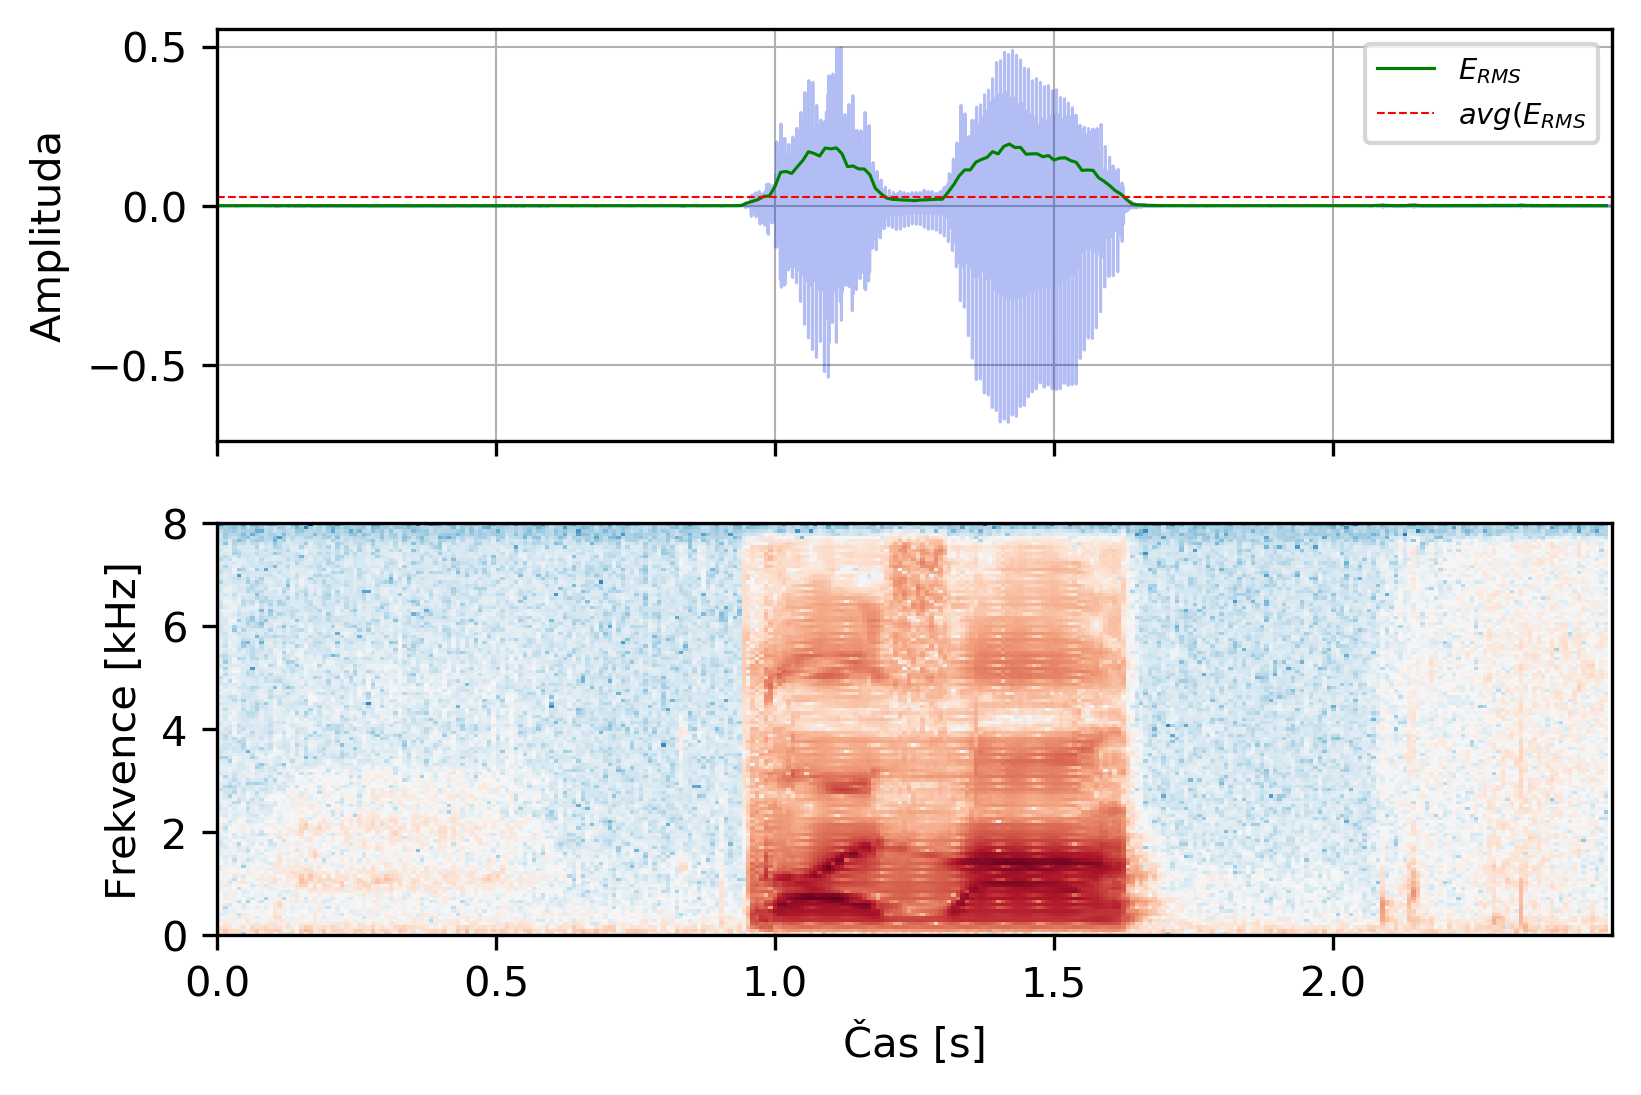
\includegraphics[width=0.9\textwidth]{./ch5-construction/img/energy_spec_word.png}
  \caption{Průběh a spektrogram slova \uv{kosa} s společně s vyznačenou energií EL promluvy.}
  \label{fig:experiments:normalization:word}
\end{figure}

\begin{figure}[hbpt]
  \centering
  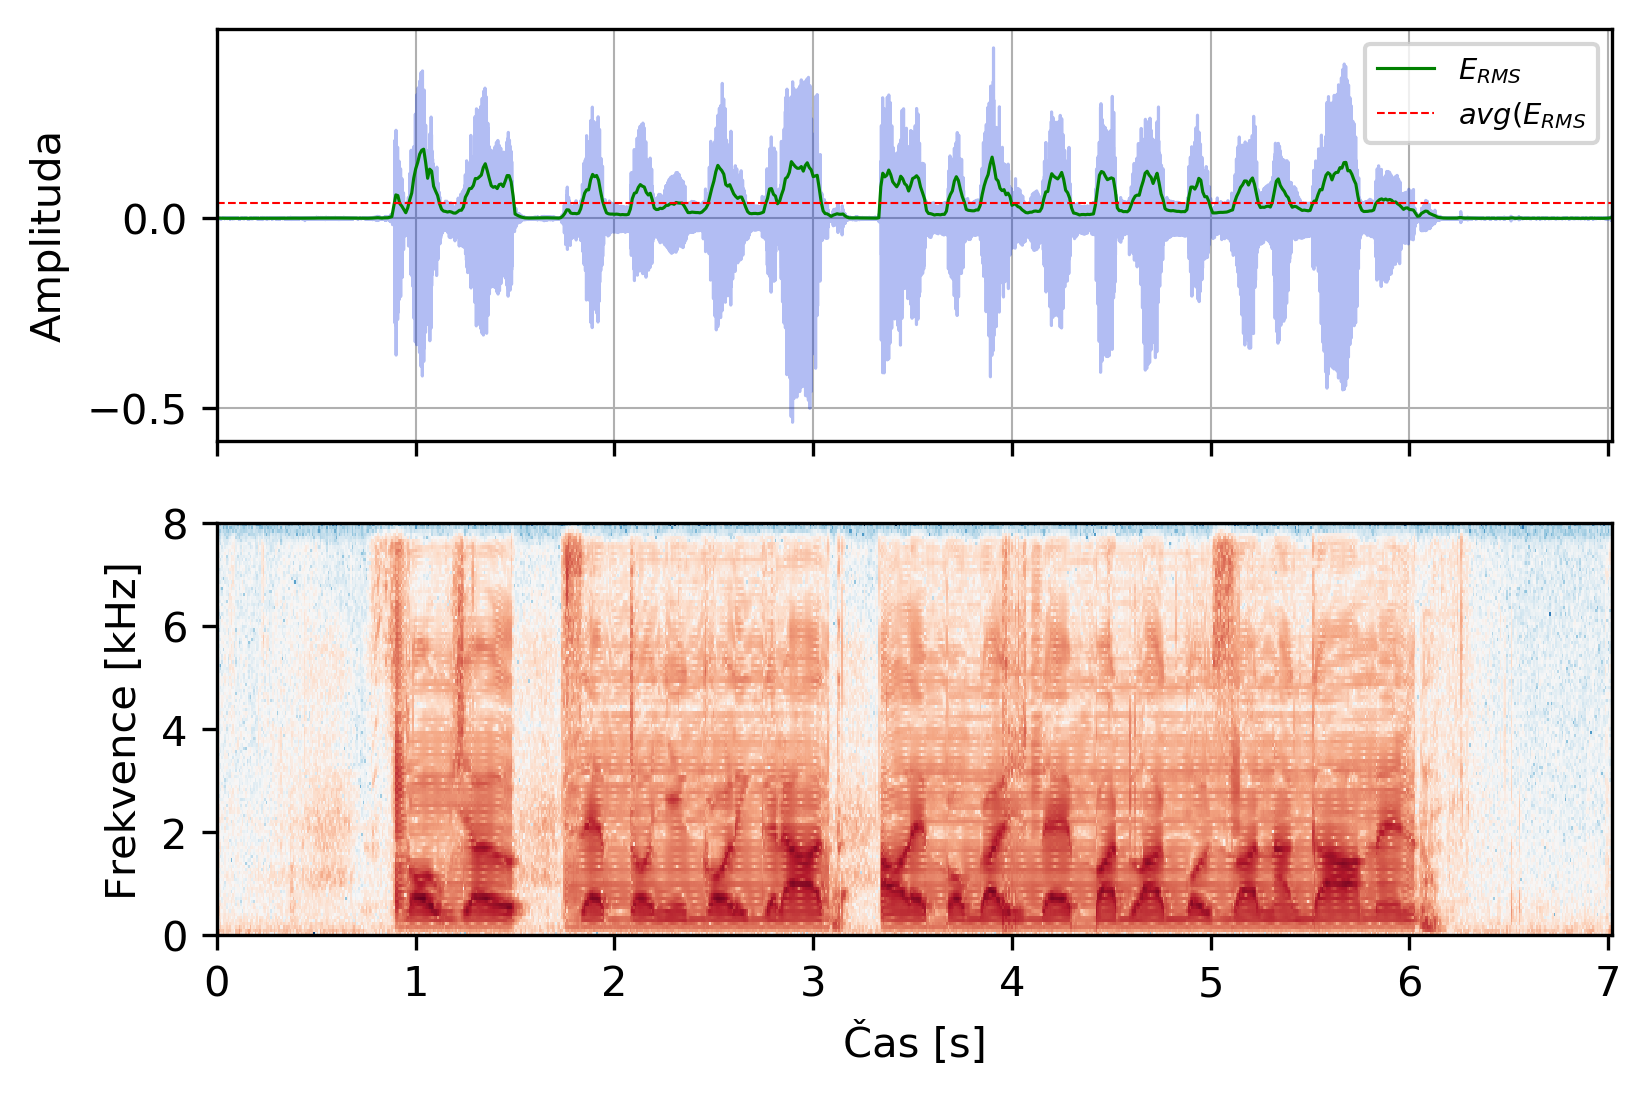
\includegraphics[width=0.9\textwidth]{./ch5-construction/img/energy_spec_sentence.png}
  \caption{Průběh a spektrogram promluvy obsahující slovo \uv{kosa} a vyznačenou energií EL promluvy.}
  \label{fig:experiments:normalization:sentence}
\end{figure}

Tab. \ref{tab:experiments:normalization:recording} přibližuje souhrnné parametry nahrávek pořízených v 2. etapě nahrávání. Celkem se pořídilo získat přibližně 2 hodiny řeči (každá nahrávka obsahuje $0,5\ s$ ticha na začátku a konci). Z toho přibližně jen $10\ \%$ představují izolovaná slova. Společně s novými daty tak korpus obsahuje téměř $14$ hodin audio záznamů a k nim příslušných přepisů.

\begin{table}[htpb]
  \centering
  \def\arraystretch{1.5}
  \pgfplotstabletypeset[
    col sep=comma,
    string type,
    columns/phase/.style={column name=Nahrávání, column type={|l}},
    columns/length/.style={column name=Délka \textit{[HH:MM:SS]}, column type={|r}},
    columns/words/.style={column name=Počet slov, column type={|r}},
    columns/sentences/.style={column name=Počet vět, column type={|r}},
    columns/files/.style={column name=Počet souborů, column type={|r|}},
    every head row/.style={after row=\hline, before row=\hline},
    every last row/.style={after row=\hline},
  ]{./ch5-construction/tabs/0201-recording-stats.csv}
  \caption{Informace o korpusu nahrávek z 2. etapy nahravání.}
  \label{tab:experiments:normalization:recording}
\end{table}

\subsection{Vliv nových dat na kvalitu modelů}
\label{chap:experiments:normalization:quality}

Mezi lety 2012 a 2016 zaznamenalo rozpoznávání řeči překotný vývoj používaných technologií. Do té doby state-of-the-art modely stavěly na kombinaci \textit{HMM} a \uv{gaussovských směsí} \textit{GMM}  U těchto modelů má každý \textit{HMM} stav svou směs, viz obr. \ref{fig:experiments:normalization:hmm:gmm}. Pravděpodobnost přechodu mezi stavy \textit{HMM} pak určují tyto směsi. Jejich parametry jsou získány na základě trénování. S příchodem open source frameworku Kaldi \cite{Kaldi2011} a rozmachem GPU výpočtů se začaly objevovat modely využívající hluboké neuronové sítě (\textit{DNN}) .

Rozpoznávání řeči je možné si představit sequence-to-sequence modely, tedy jako převod sekvence akustických parametrů do sekvence znaků/slov. Pro tento typ úloh se a priory hodí rekurentní neuronové sítě (RNN), ale jejich slabinou je enormní výpočetní náročnost i mimo trénovací fázi a také potřeba enormního množství dat, pokud má být vytvořen end-to-end\footnote{End-to-end systémem je ve valné většině případů myšlen systém, do kterého vstupuje audio framů a  vystupuje z něj sekvence znaků. Vyvojář takového systému často nepoužívá parametrizované audio.} systém \cite{Hannun2014}. Vytvoření čistě RNN end-to-end ASR systému je tak nesmírně nákladné (data, HW, atd.). V současné době se převážně využívá kombinace \textit{HMM} modelu, který je také zástupcem rodiny sequence-to-sequence modelů, a \textit{DNN}  Hlavním rozdílem oproti těm s \textit{GMM} spočívá v tom, že pro všechny \textit{HMM} stavy se trénuje pouze jedna neuronová síť, pomocí které jsou určovány přechody mezi stavy, viz obr. \ref{fig:experiments:normalization:hmm:dnn}. Navíc tím, že tato neuronová síť určuje \uv{pouze} přechody mezi jednitlivými stavy HMM, tak může být řádově menší a jednodušší, než kdyby se jednalo o end-to-end model. Tím pádem je rychleji natrénovaná a je potřeba řádově méně dat.


\begin{figure}[htpb]
  \centering
  \begin{subfigure}[b]{0.4\textwidth}
    \includegraphics[width=\textwidth]{./ch5-construction/img/HMM-GMM.pdf}
    \caption{HMM-GMM}
    \label{fig:experiments:normalization:hmm:gmm}
  \end{subfigure}
  %
  \begin{subfigure}[b]{0.4\textwidth}
    \includegraphics[width=\textwidth]{./ch5-construction/img/HMM-DNN.pdf}
    \caption{HMM-DNN}
    \label{fig:experiments:normalization:hmm:dnn}
  \end{subfigure}
  \caption{Znázornění odlišného principu \textit{HMM-GMM} a \textit{HMM-DNN}.}
  \label{fig:experiments:normalization:hmm}
\end{figure}

\subsubsection{Ověření přínosu nových dat}

S novými daty je možné natrénovat modely a ověřit, zda je s nimi systém schopen pracovat. Oproti \ref{chap:experiments:analysis:experiment} je použit framework Kaldi, který se stal standardem pro vytváření akustikých modelů. Samotný framework se skládá z velkého množství utilit, která každá plní určitý \uv{jednoduchý} úkol v procesu vytváření/testování modelu. Kompletní proces vytváření modelu se tak sestává z postupného spouštění těchto utilit v přesně definovaném pořadí. Autoři frameworku připravili nepřeberné množství skriptů, které slouží k vytvoření různých typů modelů. Všechny modely pro EL řeč vycházejí ze skriptů pro natrénování modelů z Wall Street Journal (WSJ) korpusu, který je nejčastěji požíván jako jakýsi benchmark ASR systémů. Skripty jsou jen drobně upraveny, aby výsledný model odpovídal EL doméně a bylo jej vůbec možné vytvořit.

Přestože \textit{DNN} nahradily \textit{GMM} v HMM, tak k jejich natrénování je nezbytné nejprve natrénovat \textit{HMM-GMM} model, který slouží k prvotnímu zarovnání (určení hranic jednotlivých fonémů v rámci audio náhrávky). To slouží jako startovní bod pro neuronovou síť. Tím, že je trénována pouze jedna síť, tak je k dispozici řádově více dat\footnote{V případě \textit{HMM-GMM} má každý stav své \textit{GMM} a tím pádem, čím více stavů, tím méně trénovacích dat pro každou směs.} k jejímu natrénování, na druhou stranu má tato síť mnohem více parametrů než všechny \textit{GMM} směsi dohromady a tak je potřeba dbát na velikost sítě. Nicméně pro standardní WSJ \textit{DNN} (6 vrstev, každá s 1024, 2048 nebo 4096 neurony) je dat dostatek.

Přestože vývoj výpočetních GPU postupuje závratnou rychlostí, tak natrénování standardního \textit{HMM-DNN} modelu trvá o poznání déle než \textit{HMM-GMM}. Pro ověření zda je možné vytvořit model ze všech dat, která jsou k dispozici, poslouží dobře i \textit{HMM-GMM} model, který stejně slouží jako startovní bod pro \textit{HMM-DNN}, tak by se vytvářel tak jako tak. Pokud tyto modely neposkytnou \textit{DNN}  alespoň trochu \uv{dobré} počáteční podmínky, tak sofistikovanější \textit{DNN} nemusí pomoci.

Základem procesu vytvoření modelu jsou tedy Kaldi WSJ skripty. Jako první se vytvoří monofónový akustický model. Data jsou zparametrizována pomocí Perceptual Linear Prediction (PLP) s 12 kepstrálními, delta a delta-delta koeficienty. Tento monofónový model je speciální případ kontextově závislých modelů, bez levého a pravého (fonémového) kontextu. Následně jsou natrénovány trifónové modely. Stejně jako v experimentech provedených v části \ref{chap:experiments:analysis:experiment}, tak i zde jsou použity rozhodovací stromy, protože počet všech variant trifónů je příliš velký a dat nedostatek.

V předchozí části \ref{chap:experiments:analysis:experiment} byl korpus rozdělen na trénovací a testovací sadu. Po rozšíření korpusu je rozdělení dat z 1. etapy ponecháno a nová data rozdělena mezi trénovací a testovací sadu. Všechny nahrané věty v 2. etapě jsou použity v trénovací a všechna slova naopak v testovací sadě. Toto rozdělení je logické, protože důvodem rozšíření korpusu je snaha ověřit funkčnost ASR systémů na slovech, která mají rozdílný význam, ale liší se pouze znělostí jednoho fonému. Jelikož z výsledků v části \ref{chap:experiments:analysis:reduction} vyplývá, že určité spektrum trifónů je možné reprezentovat pouze pomocí znělých variant, tak při použití nahraných slov bude teoreticky možné lépe prozkoumat tuto otázku.

Pro otestování výše popsaného modelu je opět použit monofónový zerogramový jazykový model tak, aby co nejméně ovlivňoval dosažené výsledky. Na kompletní testovací sadě byla dosažena přesnost $54,96\ \%$. V případě, že testovací sada obsahovuje pouze nově nahraná slova, tak dokonce jen $42,97\ \%$. Což je významné zhoršení oproti výsledkům dosažených v \ref{chap:experiments:analysis:experiment}, kde bylo dosaženo více něž $80\ \%$ přesnosti. Pro výpočet přesnosti je ve všech případech použita rovnice \ref{eq:experiments:analysis:experiment:accuracy}.

Pro ověření, že není chyba v procesu trénování (přeci jen se změnil framework) poslouží křížový test, kdy pomocí stejného procesu jsou natrénovány modely z původních (1. etapa) a nových (2. etapa) dat a křížově otestovány na kompletní, původní a jen nové části testovací sady. Výsledky tohoto testu jsou v tab. \ref{tab:experiments:normalization:cross}. Z té je jasně patrné, že pokud je model natrénován a otestován pomocí dat pocházející ze stejné etapy, tak je dosaženo podobných výsledků jako v \ref{chap:experiments:analysis:experiment}. Trénovcací proces je tedy \uv{správný}.

%model;orig;new

\begin{table}[htpb]
  \centering
  \def\arraystretch{1.5}
  \pgfplotstabletypeset[
    col sep=semicolon,
    string type,
    columns/model/.style={column name=Model, column type={|c}},
    columns/orig/.style={column name=1. etata $[\%]$, column type={|r}},
    columns/new/.style={column name=2. etapa $[\%]$, column type={|r|}},
    every head row/.style={before row={
      \hline
      & \multicolumn{2}{c|}{Accuracy} \\
    },after row=\hline},
    every last row/.style={after row=\hline},
  ]{./ch5-construction/tabs/0202-cross_test.csv}
  \caption{Křížový test modelů natrénovaných a otestovaných na datech z 1. a 2. etapy.}
  \label{tab:experiments:normalization:cross}
\end{table}

% - 20161208_param -> porovnani n vs o, vzit hodnoty z toho
% - 20170111_together -> \textit{CMN}  FULL vysledky na HMM, pak tam dat i vysledky z

\subsubsection{Eliminace vlivu kanálu}

Z prezentovaných výsledků tedy plyne, že nová data jsou příliš odlišná od původních a v parametrickém prostoru příliš vzdálena těm původním. Zároveň je těchto dat relativně malé množství, aby se mohly modely plně adaptovat. Na zmíněný rozdíl v datech je možné se koukat jako na změnu kanálu, která je příčinou těchto změn. Řečník je přeci stejný. V předchozím textu bylo zmíněno, že v rámci 2. etapy došlo ke změné nahrávací procedury a také elektrolarynxu. Tím byl pozměněn kanál a logicky výsledná zaznamenaná řeč má jiné parametry než ta v 1. etapě. Mezi další prvky, které mohou způsobit změnu kanálu může být prostředí, tedy jestli je řeč produkována uvnitř nějaké místnosti, či venku, jestli je na pozadí přítomen šum atd. K tomu, aby bylo možné použít všechna dostupná data, je potřeba eliminovat tento vliv kanálu. K jeho eliminaci se standardně používá \textit{CMN},  což je zkratka anglických slov Cepstral Mean Normalisation. Principem této metody je odstranení vlivu kanálu na základě střední hodnoty kepstrálních koeficientů, viz dále.

Zaznamenaný signál je možné popsat jako konvoluci promluvy a vlivu kanálu, matematicky zapsáno jako

\begin{equation}
  y\left[n\right] = x\left[n\right] \circledast h\left[n\right],
  \label{eq:experiments:normalization:convolution}
\end{equation}

\noindent kde $x\left[n\right]$ představuje vstupní signál, tedy řeč, a $h\left[n\right]$ odezvu kanálu na jednotkový impulz. Zaznamenaný signál je jejich již zmíněnou lineární konvolucí. Ve frekvenční oblasti je pak rovnice \ref{eq:experiments:normalization:convolution} zapsaná následovně:

\begin{equation}
  Y\left[f\right] = X\left[f\right] \cdot H\left[f\right]
\end{equation}

\noindent V této oblasti se z konvuluce stalo násobění, což značně zjednodušuje situaci. K odstranění vlivu kanálu je, ale ještě potřeba převést hodnoty do kepstrálná oblasti. To je realizováno pomocí logaritmu spektra

\begin{equation}
  Y\left[q\right] = \log\left(Y\left[f\right]\right) = \log\left(X\left[f\right] \cdot H\left[f\right]\right) = X\left[q\right] + H\left[q\right],
\end{equation}

\noindent kde $q$ představuje kepstrální koeficient. V kepstrální oblasti je vliv kanálu aditivní složkou výsledného záznamu. Problémem však je, že konkrétní hodnota vlivu kanálu je neznáma, protože k dispozici je pouze výsledný ovlivněný signál. Předpokládejme však, že vliv kanálu je stacionární\footnote{Jedná se sice o silný, ale logický předpoklad. Pokud se vztáhne k pořízenému řečovému korpusu, tak v rámci jedné etapy nahrávání, je proces nahrávání neměnný, tzn. je použita stejná aparatura a k nahrávání dochází vždy ve stejné místnosti.}, tak poté je možné každý frame nahrávky $i$ zapsat jako

\begin{equation}
  Y_i\left[q\right] = H\left[q\right] + X_i\left[q\right],
\end{equation}

\noindent kde $Y_i\left[q\right]$ představuje $i$ frame kepstra $q$ nahrávky a $X_i\left[q\right]$ představuje $i$ frame kepstra $q$ neovlivněné řeči. Z této rovnice je pak možné vypočítat střední hodnotu

\begin{equation}
  \frac{1}{N} \sum_i Y_i\left[q\right] = H\left[q\right] + \frac{1}{N} \sum_i X_i\left[q\right].
\end{equation}

\noindent Vliv kanálu je následně možné eliminovat odečtením střední hodnoty kepstra $q$ od aktuální hodnoty kepstra $Y_i\left[q\right]$

\begin{align}
  R_i\left[q\right] &= Y_i\left[q\right] - \dfrac{1}{N}\sum_{j} Y_j\left[q\right] \nonumber  \\
  &= H\left[q\right] + X_i\left[q\right] - \left( H\left[q\right] + \frac{1}{N} \sum_j X_j\left[q\right] \right) \nonumber  \\
  &= X_i\left[q\right] - \frac{1}{N} \sum_j X_j\left[q\right]
  \label{eq:experiments:normalization:cmn}
\end{align}

\noindent S pomocí rovnice \ref{eq:experiments:normalization:cmn} je možné odfiltrovat vliv kanálu a teoreticky tak získat hodnoty kepstrálních koeficientů odpovídající nezkreslené řeči. Otázkou je, přes jaký úsek počítat střední hodnotu. Je možné ji počítat přes posuvné okénko fixní délky, přes jednotlivé nahrávky, nebo dokonce přes všechny nahrávky konkrétní etapy. Pokud totiž bude úsek, přes který je počítána průměrná hodnota, krátký, tak se může stát, že vypočtená střední hodnota nebude odpovídat skutečné střední hodnotě umožňující eliminaci vlivu kanálu. V tomto případě, kdy nahrávky dělí velký časový úsek a i proces nahrávání byl změněn, je toto potřeba odexperimentovat.

Pro zjištění jaká možnost je optimální je použit stejná trénovací procesdura jako v předešlých experimentech s novými daty. Jediný rozdíl je v datech, na kterých bylo aplikováno \textit{CMN}.  Celkem byly uvažovány dva experimenty, a to

\begin{itemize}
  \item \textit{CMN}  počítáno pro každou nahrávku,
  \item \textit{CMN}  počítáno pro celou etapu,
\end{itemize}

\noindent algoritmus \textit{CMN}  aplikovaný na datech byl implementován na katedře kybernetiky Fakulty aplikovaných věd.

V tab. \ref{tab:experiments:normalization:cmn:file} jsou výsledky experimentu s \textit{CMN}  počítaném přes jednotlivé nahrávky. Z dosažených výsledků je zřejmé, že pokud se \textit{CMN}  počítá přes jednotlivé nahrávky, tak je oproti výsledkům v tab. \ref{tab:experiments:normalization:cross} dosaženo určitého zlepšení, zvláště pokud je model natrénován na datech z 1. etapy a otestován na datech z 2. etapy, ale výsledky nejsou zdaleka tak dobré, jako v případě, že je model natrénován a otestován na datech ze stejné sady. Vliv tu může hrát fakt, že zejména nahrávky izovlovaných slov jsou relativně krátké a vypočtené střední hodnoty, tak nabývají odličných hodnot.

\begin{table}[htpb]
  \centering
  \def\arraystretch{1.5}
  \pgfplotstabletypeset[
    col sep=semicolon,
    string type,
    columns/model/.style={column name=Model, column type={|c}},
    columns/orig/.style={column name=1. etata $[\%]$, column type={|r}},
    columns/new/.style={column name=2. etapa $[\%]$, column type={|r|}},
    every head row/.style={before row={
      \hline
      & \multicolumn{2}{c|}{Accuracy} \\
    },after row=\hline},
    every last row/.style={after row=\hline},
  ]{./ch5-construction/tabs/0203-cmn_file.csv}
  \caption{Křížový test modelů natrénovaných a otestovaných na datech z 1. a 2. etapy s \textit{CMN}  přes jednotlivé soubory.}
  \label{tab:experiments:normalization:cmn:file}
\end{table}

Další experiment je tedy s daty, kde bylo \textit{CMN}  vypočteno ze všech nahrávek konkrétní etapy. V tab. \ref{tab:experiments:normalization:cmn:full} je vidět markantní zlepšení výsledků. Pokud je model natrénován na datech z 1. etapy a otestován na datech z libovolné etapy, tak jsou dosažené výsledky velmi podobné. Nejhoršího výsledku je dosaženo, pokud je model natrénován na datech z 2. etapy a otestován na těch z té 1. V tomto případě hraje velký vliv, že model je natrénován z relativně malého množství dat (pouhé 2 hodiny). Pokud je tedy \textit{CMN}  počítáno přes všechny nahrávky v etapě, tak je dosaženo významného zlepšení a vliv kanálu je v podstatě eliminován. Pro doplnění je dobré zmínit, že pokud je model natrénován ze všech trénovacích dat (1. a 2. etapa) a otestován pomocí kompletní testovací sady, tak je dosažená přesnost s monofónovým zerogramovým jazykovým modelem rovna $77,69\ \%$, což je výsledek přibližující se hodnotám dosaženým v prvnotních experimentech v části \ref{chap:experiments:analysis:experiment}.

\begin{table}[htpb]
  \centering
  \def\arraystretch{1.5}
  \pgfplotstabletypeset[
    col sep=semicolon,
    string type,
    columns/model/.style={column name=Model, column type={|c}},
    columns/orig/.style={column name=1. etata $[\%]$, column type={|r}},
    columns/new/.style={column name=2. etapa $[\%]$, column type={|r|}},
    every head row/.style={before row={
      \hline
      & \multicolumn{2}{c|}{Accuracy} \\
    },after row=\hline},
    every last row/.style={after row=\hline},
  ]{./ch5-construction/tabs/0204-cmn_full.csv}
  \caption{Křížový test modelů natrénovaných a otestovaných na datech z 1. a 2. etapy s \textit{CMN}  přes všechny nahrávky v etapě.}
  \label{tab:experiments:normalization:cmn:full}
\end{table}

Z výsledků v tab. \ref{tab:experiments:normalization:cmn:file} je možné odvodit, že pokud se \textit{CMN}  počítá přes posuvné okénko fixní délky, tak dosažené výsledky nejsou zrovna dobré. Což se i experimentálně potvrdilo, když výsledná přesnost dosáhla hodnoty $56,51\ \%$, pokud jsou použita všechna data. Nicméně framework Kaldi umožňuje aplikování CMVN, což je Cepstral mean and variance normalization. Oproti standardními \textit{CMN}  je uvažována i variance v kepstrální oblasti. Technicky je pravá část rovnice \ref{eq:experiments:normalization:cmn} ještě podělena vypočtenou variancí daného kepstrálního koeficientu $q$. Takže pokud je použito Kaldi CMVN, tak výsledná přesnost, na modelu trénovaném a testovaném na všech datech, dosáhla hodnoty $76,15\ \%$. Tento výsledek je srovnatelný s modelem využívající \textit{CMN}  přes všechny nahrávky v dané etapě.

Po zjištění vhodného nastavení \textit{CMN},  pro odfiltrování vlivu kanálu, je dalším krokem natrénování neuronové sítě. V předchozím textu bylo zmíněno, že neuronová síť jako počáteční podmínky používá zarovnání získané pomocí \textit{GMM}  To je získáno díky natrénovaným modelům s \textit{CMN}  přes všechny nahrávky. Trénovaná neuronová síť je typu fully connected feedforward s 6 vrstvami (5 skrytých vrstev). Postupně je natrénována síť s 1024, 2048 a 4096 neurony v každé vrstvě, výstupní vsrva je typu softmax s dimenzí rovnou počtu \textit{HMM} stavů. Jazykový model je stejně jako u všech předchozím experimentů monofónový zerogramový. Tab. \ref{tab:experiments:normalization:dnn} ukazuje dosažené výsledky všech natrénovaných variant. Nejvyšší přesnosti dosahuje model s 4096 neurony v každé vrstvě, ale rozdíl od ostatních variant není velký. Oproti nejlepšímu \textit{GMM} modelu \textit{DNN} síť přidala dalších $6,97\ \%$ absolutně.

\begin{table}[htpb]
  \centering
  \def\arraystretch{1.5}
  \pgfplotstabletypeset[
    col sep=semicolon,
    string type,
    columns/neurons/.style={column name=Počet neuronů, column type={|c}},
    columns/accuracy/.style={column name=Accuracy $[\%]$, column type={|r|}},
    every head row/.style={before row=\hline,after row=\hline},
    every last row/.style={after row=\hline},
  ]{./ch5-construction/tabs/0205-dnn.csv}
  \caption{Dosažená přesnost neuronové sítě s monofónovým zerogramovým jazykovám modelem.}
  \label{tab:experiments:normalization:dnn}
\end{table}

\subsection{Poslechový test}
\label{chap:experiments:normalization:listening}

V předchozím textu byly prezentovány různé dosažené výsledky, ale ty zatím nedokázali odpovědět na zásadní otázku: \uv{Dokáže se stroj\footnote{Stroj je zde reprezentován systémem automatického rozpoznávání řeči.} vyrovnat človéku?}. Přestože je EL řeč na první poslech obtížně srozumitelná, tak již po krátké době je člověk schopný obstojně poruzumnět. S přibývajícím časem se do určité míry porozumnéní ještě zlepšuje. Jak je na tom tedy stroj v porovnání s člověkem?

Ještě než je vůbec možné na tuto otázku odpovědět, tak je dobré si odpovědět na otázku: \uv{Jakým způsobem porovnat schopnosti člověka a stroje?}. K tomu může posloužit poslechový test, ve kterém mají posluchačí za úkol určit, z předem definovaných možností, co je obsahem promluv. Otestování schopností stroje pak probíhá pomocí experimentu, kde na vstupu systému jsou stejné promluvy, která jsou součástí poslechového testu, a výstupem je přepis. Metrika je pak počítána na základě správně/špatně určeného obsahu promluv. Prostým porovnáním správně určeného obsahu člověka a stroje je pak možné odpovědět na první \uv{položenou} otázku.

Při přípravě experimentu vykrystalizovaly tyto varianty poslechového testu:

\begin{itemize}
  \item test na izolovaných slovech,
  \item test na slovních bigramech.
\end{itemize}

\noindent Tím, že promluvy obsahují pouze izolovaná slovo (v druhém případě dvojici slov) je do značné míry eliminován vliv kontextu. Ten v mnohých případech pomáhá se správným určením významu slova i přesto, že nebylo dobře rozumnět. Pokud se bude navíc experiment skládat z množiny promluv, která obsahuje pouze slova popsaná v části \ref{chap:experiments:normalization:corpus}, tak je možné  určit jak \uv{dobře} je člověk (stroj) určit význam a případně od sebe odlišit tato slova.

\subsubsection{Izolovaná slova}

Určení významu slova, které bylo vysloveno v klidném prostředí se jeví jako velice jednoduchý úkol, ale pokud jej vyslovil řečník používající EL, tak už to tak snadné být nemusí, zvlášť pokud se jedná o slova v popsaná v \ref{chap:experiments:normalization:corpus}. V tomto případě mají účastníci poslechového testu za úkol postupně vyslechnout $320$ nahrávek izolovaných slov a vybrat jednu z předem definovaných odpovědí:

\begin{enumerate}[label=\alph*)]
  \item slovo A \textit{(např. kosa)},
  \item slovo B \textit{(např. koza)},
  \item nemohu rozhodnout.
\end{enumerate}

\noindent Ve výčtu možností je vždy skutečně pronesené slovo a k němu pak varianta lišící se pouze znělostí jednoho fonému. První dvě možnosti jsou vždy v abecedním pořadí. Nahrávky použité v rámci poslechového testu odpovídají nahraným slovům v rámci 2. etapy nahrávání. Poslechového testu se účastnilo $19$ subjektů z řad kolegů.

Výstupem poslechového testu je tabulka s procentuálním zastoupením jednotlivých odpovědí pro každou nahrávku. V tab. \ref{tab:experiments:normalization:isolated} je zobrazen výňatek získaných výsledků. Správné odpovědi jsou zvýrazněny tučně. První příklad reprezentuje situaci kdy účastník nebyl jednoznačně schopen určit význam slova. Druhý příklad pak ukazuje situaci, kdy všichni účastníci vybrali z komplementárních slov vždy pouze jediné, a to nehledě na to, které jim bylo ve skutečnosti puštěno. V tomto konkrétním případě tedy posluchači vždy \uv{slyšeli} slovo \uv{koza}. Dalo by se tedy usuzovat, že slova \uv{kosa} je akusticky identické se slovem \uv{koza}. Poslední případ reprezentuje situaci, kdy většina účastníků byla schopna určit správně význam slova. Celková přesnost pak dosáhla hodnoty $Acc_w^{human} = 70,47\ \%$ a byla vypočtena pomocí následujícího vzorce

\begin{equation}
  Acc_w^{human} = \frac{1}{n} \sum_{i=1}^{N} f_i * 100,
  \label{eq:experiments:normalization:accuracy:human}
\end{equation}

\noindent kde $n=320$ a $f_i$ se rovná relativní frekcenci správných odpovědí na otázku $i$ v poslechovém testu s izolovanými slovy.

\begin{table}[htpb]
  \centering
  \def\arraystretch{1.5}
  \pgfplotstabletypeset[
    col sep=semicolon,
    string type,
    columns/word/.style={column name=Slovo, column type={|l}},
    columns/option1/.style={column name=Možnost \textit{\textbf{a)} [\%]}, column type={|r}},
    columns/option2/.style={column name=Možnost \textit{\textbf{b)} [\%]}, column type={|r}},
    columns/option3/.style={column name=Možnost \textit{\textbf{c)} [\%]}, column type={|r|}},
    every head row/.style={after row=\hline, before row=\hline},
    every row no 1/.style={after row=\hline},
    every row no 3/.style={after row=\hline},
    every last row/.style={after row=\hline},
  ]{./ch5-construction/tabs/0206-isolated.csv}
  \caption{Ukázka výsledku poslechového testu na izolovaných slovech.}
  \label{tab:experiments:normalization:isolated}
\end{table}

\subsubsection{Slovní bigramy}

V druhém poslechovém testu mají za úkol vyslechnout $333$ nahrávek slovních bigramů\footnote{Nahrávky obsahují dvě po sobě vyslovená slova.} a vybrat jednu z předem definovaných odpovědí. Ty mají vždy následující formát

\begin{enumerate}[label=\alph*)]
  \item slovo A + slovo A \textit{(např. kosa + kosa)},
  \item slovo A + slovo B \textit{(např. kosa + koza)},
  \item slovo B + slovo A \textit{(např. koza + kosa)},
  \item slovo B + slovo B \textit{(např. koza + koza)}.
\end{enumerate}

\noindent Je zřejmé, že to představuje všechny kombinace, které lze z dvojice vytvořit. Dvojice slov vždy tvoří již několikrát zmíněné dvojice slov mající jiný význam, ale lišící se právě v jednom fonému. Rozšířený řečový korpus, tak jak je popsaný v části \ref{chap:experiments:normalization:corpus}, ale neobsahuje tento typ nahrávek. Tím pádem je potřeba je vytvořit \uv{uměle}. Což není velký problém, protože každá nahrávka izolovaného slova obsahuje minimálně $0,5\ s$ ticha na začátku a konci. Pokud jsou tyto nahrávky spojeny\footnote{Ke spojení je možné použít nástroj \textit{ffmpeg} nebo \textit{sox}.}, vznikne jediná nahrávka obsahující dvě zájmová slova oddělena krátkou pauzou. Z každé dvojice slov vznikly vždy dvě nahrávky lišící se pořadím slov.

Vyšší počet položek v testu je zapříčiněn faktem, že pro určitá slova existuje více než jedna kombinace s jiným slovem\footnote{Ve valné většině se jedná o slova obsahující písmena \textit{i/y}, která jsou v akustické formě identická. Příkladem může být dvojice \textit{nebyli + nepili} a \textit{nebili + nepili}.}. Ve snaze zkrátit, už tak docela náročený poslechový test, byly vygenerovány bigramy odpovídající poiuze možnostem \textit{b)} a \textit{c)}. Účastníci poslechového testu o tom však nebyli informováni. Přesto tento poslechový test dokončilo pouze $12$ účastníků.

Stejně jako u testu s izolovanými slovy je výstupem testu tabulka obsahující procentuální zastoupení jednotlivých odpovědí na každou otázku. Tab. \ref{tab:experiments:normalization:bigrams} obsahuje ukázku těchto výsledků. Stejně jako v předchozím případě, správné odpovědi jsou zvýrazněny tučně. Ačkoli jsou nyní v testu dvojice slov, tak dosažené výsledky do značné míry korespondují s výsledky z testu s izolovanými slovy (viz tab. \ref{tab:experiments:normalization:isolated}). V prvním případě (\textit{borci + porci}) nebyli účastníci schopni jednoznačně určit význam slov v nahrávce, stejně jako v případě testu na izolovaných slovech. V druhém případě (\textit{kosa + koza}) všichni posluchači až na jednoho vybrali možnost \textit{d)}, tedy \textit{koza + koza}. Správný výběr jedním účastníkem lze považovat spíše za náhodu, protože v případě opačného pořadí slov již nikdo správnou odpověď nevybral. Je dobré zmínit, že účastníci v žádném poslechovém testu nebyli omezeni v počtu opětovného přehrání promluvy. Tím pádem je velmi pravděpodobné, že tento konrétní participant opakovaně poslouchal danou nahrávku a hledal rozdíl až nějaký drobný zaznamenal. Otazkou však je jestli to spíš nebyla sugesce a to již zmíněné štěstí.

Poslední prezentovaný příklad zastupuje množinu odpovědí, kdy účastníci naprosto správně určili význam slov. Průměrná dosažená přesnost člověka, počítána pomocí rovnice \ref{eq:experiments:normalization:accuracy:human}, dosáhla hodnoty $Acc_{p}^{human} = 66,24\ \%$.

\begin{table}[htpb]
  \centering
  \def\arraystretch{1.5}
  \pgfplotstabletypeset[
    col sep=semicolon,
    string type,
    columns/word/.style={column name=Slovní bigram, column type={|l}},
    columns/option1/.style={column name=Mož. \textit{\textbf{a)} [\%]}, column type={|r}},
    columns/option2/.style={column name=Mož. \textit{\textbf{b)} [\%]}, column type={|r}},
    columns/option3/.style={column name=Mož. \textit{\textbf{c)} [\%]}, column type={|r}},
    columns/option4/.style={column name=Mož. \textit{\textbf{d)} [\%]}, column type={|r|}},
    every head row/.style={after row=\hline, before row=\hline},
    every row no 1/.style={after row=\hline},
    every row no 3/.style={after row=\hline},
    every last row/.style={after row=\hline},
  ]{./ch5-construction/tabs/0207-bigrams.csv}
  \caption{Ukázka výsledku poslechového testu na dvojicích slov.}
  \label{tab:experiments:normalization:bigrams}
\end{table}

\subsection{Výsledky porovnání}
\label{chap:experiments:normalization:comparison}

Výsledky poslechového testu ukázaly jak je na tom člověk. Nyní je potřeba zjistit jak je na tom vlastně stroj. K tomu je nezbytné natrénovat akustický model a použít vhodný jazykový model. Jako akustický model je použitá neuronová síť popsaná v části \ref{chap:experiments:normalization:quality}. Jedná se tedy o \textit{DNN} s $6$ vrstvami ($5$ skrytých vrstev, každá s $4096$ neurony), výstupní vrstva je typu softmax s dimenzí rovnou počtu \textit{HMM} stavů. Jako parametrizace je použito PLP (statické + delta + delta-delta parametry) a pro eliminaci vlivu kanálu pak \textit{CMN}.  Výsledný příznakový vektor má dimenzi $40$ (viz část \ref{chap:experiments:analysis:reduction}). Vstupem neuronové sítě je pak parametrizované okénko mající kontext přes $5$ framů\footnote{Celkem je $5$ framů předchazející a $5$ následující aktuální frame.}. Vstupní dimenze neuronové sítě je tedy $440$. K natrénování takovéhoto modelu je použit framework Kaldi. Oproti dosavadním experimentům je v tomto případě použit vlastní real-time dekodér. Tento LVCSR systém je optimalizován pro co nejnižší latenci a je schopný pracovat velmi velkými slovníky, čítající miliony položek. Tento dekodér byl vyvinut na katedře kybernetiky Fakulty aplikovaných věd.

Z poslechových testů jsou k dispozici dva výsledky. První reprezentuje schopnost určit význam izolovaného slova. Druhý pak schopnost od sebe rozeznat dvě velmi podobná slova. Pro potřeby porovnat tyto výsledky s těmi dosaženými ASR systémem jsou vytvořeny celkem $3$ experimenty využívající výše popsaný Kaldi model.

První experiment odpovídá poslechovému testu s izolovanými slovy a jeho základem je zerogramový LM obsahující více než 1 milion slov. Většina předchozích experimentů využívala monofónový zerogramový model, aby bylo možné eliminovat jeho vliv na výsledné přesnosti. U těchto experimentů je, ale tento LM nevyhovující, protože cílem je správně rozpoznat celé slovo, a proto je využit slovní jazykový model. U zerogramového modelu mají všechny položky stejnou pravděpodobnost, tím je zaručeno, že nebudou preferována četnější slova. Data pro tento LM pocházejí z novinových článků, webových zpravodajských serverů, filmových titlků a přepisů televizních pořadů. Využití takto velkého LM vychází z představy, že i člověk má velkou slovní zásobu a dopředu neví co bude obsahem konkrétní promluvy v rámci testu. Tento test je pojmenován jako \uv{onemil}.

Ve skutečnosti však, v rámci poslechového testu, účastníci znají seznam slov zahrnutých do testu a mají tak určitou výhodu oproti \uv{onemil} nastavení. Ke kompenzaci tohoto faktu, je vytvořen druhý experiment, který má redukovaný LM. Ten obsahuje pouze slova, která se opravdu vyskytla v rámci poslechového testu. Tento experiment je nazván jako \uv{reduced}. Výsledky obou těchto experimentů jsou porovnány s poslechovým testem na izolovaných slovech. Další možností by mohlo být vytvoření speciálních LM pro každou promluvu obsahující pouze komplementární slova. Bohužel problémem je, že poslechový test obsahuje ještě 3 možnost (\uv{nemohu rozhodnout}) a v případě, že by LM obsahoval pouze dvě slova, tak by ASR experiment, svými parametry, neodpovídal poslechovému testu.

Poslední experiment odpovídá druhému poslechovému testu. K získání srovnatelných výsledků, je pro každý slovní bigram vygenerován speciální zerogramový LM. Ten obsahuje vždy pouze všechny 4 kombinace slov. Tím pádem odpovídá dostupným možnostem v rámci druhého poslechového testu. Tento experiment je nazván jako \uv{bigrams} a jeho výsledky jsou porovnány s druhým poslechovým testem.

Výsledkem rozpoznávače je nejlepší hypotéza (případně \textit{N} nejlepších hypotéz), tudíž slovo. To však není porovnatelné s výsledkem poslechového testu. Z tohoto důvodu jsou všechny výsledky systému ASR ohodnoceny $1$, pokud bylo výstupem správné slova, v opačném případě pak $0$. Násladně byl z tohoto ohodnocení vypočten průměr. Pro upřesnějí je nutné zmínit, že \textit{i/y} na výsledném ohodnocení nehraje roli. Dosažené výsledky jsou pak v tab. \ref{tab:experiments:normalization:comparison}. Ty ukazují, že požedovaný úkol je výzvou i pro samotného člověka, natož pro stroj. V případě experimentu \uv{onemil} je výkon ASR systému významně horší než výkon člověka. To je zejména způsobeno enormní perplexitou jazykového modelu. Ta je přímo rovna velikosti slovníku. Zmenšením slovníku se podařilo získat výsledky srovnatelné s člověkem. Je dobré zdůraznit, že i v případě \uv{reduced} experimentu hrají karty ve prospěch člověka, protože čelí pouze perplexitě $3$, protože se kdykoli může podívat na nabízené možnosti. Řešením by bylo nechat účastníky přepsat obsah promluvy a porovnat ho se skutečným obsahem. Nicméně toto by významně zvýšílo náročnost (zejména časovou) poslechového testu a bylo by velmi komplivané získat kompletní výsledky od relevantního množství účastníků. Už jen podíl odpadlíků mezi prvním a druhým poslechovým testem činil závratných $30\ \%$.

Velmi zajímavé jsou výsledky u \uv{bigrams} experimentu. Na první pohled se může jevit jako snazší, protože úkolem je vybrat z jasně definovaných kombinací slov. Avšak slova jsou si akusticky velmi podobná a v mnoha případech je velmi náročné je od sebe rozeznat. Jak člověk, tak stroj, dosáhli v tomto testu nejhorších výsledků. Při analýze se ukázalo, že rozdíly mezi hypotézami ASR systému jsou velmi malé, což naznačuje velkou podobnost mezi inkriminovanými modely fonémů. Zároveň tyto výsledky s velmi podobnými hypotézami korelují s výsledky poslechového testu, kde posluchači nebyli schopni jednoznačně rozhodnout o významu jednotlivých slov.

\begin{table}[htpb]
  \centering
  \def\arraystretch{1.5}
  \pgfplotstabletypeset[
    col sep=semicolon,
    string type,
    columns/type/.style={column name= , column type={|l}},
    columns/onemil/.style={column name=onemil \textit{[\%]}, column type={|r}},
    columns/reduced/.style={column name=reduced \textit{[\%]}, column type={|r}},
    columns/bigrams/.style={column name=bigrams \textit{[\%]}, column type={|r|}},
    every head row/.style={after row=\hline, before row=\hline},
    every last row/.style={after row=\hline},
  ]{./ch5-construction/tabs/0208-comparison.csv}
  \caption{Porovnání dosažených výsledků člověka a stroje.}
  \label{tab:experiments:normalization:comparison}
\end{table}

Z dosažených výsledků je zřejmé, že stroj nedosahuje schopností člověka. Pokud se vezme v úvahu, že byl člověk oproti stroji vždy v malé výhodě, tak dosažené výsledky jsou relativně optimistické, protože minimálně v jednom případě se stroj téměř vyrovnal člověku. Samotnou kapitolou je vliv kontextu. Ještě před samotnými ASR experimenty byl ověřen výkon ASR systému na \uv{kontinuální} řeči, zde reprezentované větami z testovací sady. Jazykovým modelem je v tomto případě trigramový model obsahující $1,2$ milionu unikátních slov. Přesnost na slovech (počítaná pomocí rovnice \ref{eq:experiments:analysis:experiment:accuracy}) dosáhla hodnoty $86,10\ \%$. Při porovnání s výsledky z tab. \ref{tab:experiments:normalization:comparison} jasně plyne, že pokud je k dispozici dostatečný kontext, tak je ASR schopen správně určit význam slova. Přeci jen slovo \uv{kosa} se většinou vyskytuje v trochu jiném slovním kontextu než slovo \uv{koza} a toto platí u většiny dvojic.

% !TEX root = ../thesis.tex
\section{Augmentace dat}
\label{chap:experiments:augmentation}

Poslechový test jasně uázal, že správné rozpoznání pronesené EL promluvy není lehký úkol ani pro člověka. Naprosto markantní význam hraje kontext. Ten velmi významně pomáhá, pokud některá část promluvy nebyla dobře rozumnět nebo bylo těžké ji porozumnět. Navíc, ze zkušeností získaných při pořizování řečového korpusu (části \ref{chap:experiments:analysis:corpus} a \ref{chap:experiments:normalization:corpus}), plyne, že EL řečník má tendenci mluvit ve spíše kratších dávkách slov, mezi kterými dělá drobné pauzy. V tomto případě pro člověka není problém udržet v povědomí kontext, ale stroji to může někdy způsobovat problémy. Otázkou tedy je, jak \uv{vylepšit} stroj tak, aby poskytoval lepší výsledky?

Ať se řečník snaží sebevíc, tak se současnými metodami rehabilitace hlasu (viz \ref{sec:cause:treatment}), se při ztrátě hlasivek část informace z produkované řeči ztrácí. Obnovit tuto informaci se snaží valná většina prezentovaných přístupů v části \textbf{TBD}. Ve valné většině případů se k tomu využívá obohacení modelu o artikulační data, nebo dokonce využití jen těchto artikulačních dat. \cite{Denby2010} \cite{Hofe2013} Problém s ní je ale v tom, že ne všechny akustické nuance mezi podobnými fonémy nejsou artikulací vůbec ovlivněny. Navíc její záznam s sebou nese používaní dalšího zařízení (kamery, ultrazvuku \cite{Hueber2010}), nebo dokonce nutnost podstoupení dalšího operačního zákroku (magnety \cite{Hofe2011}). Samozřejmě je férové říct, že většina těchto vyvíjených systémů si klade za cíl komletně nahradit současné metody rehabilitace. Na druhou stranu faktem je, že ani po dlouholetém vývoji se většina těchto systémů nedostala z raně vývojové fáze. Nepochybně hraje určitou roli i to, že je tato problematika přeci jen na okraji zájmu řečařské komunity.

Pokud tedy není úplně reálné získat ztracenou informaci pomocí kompletní změny paradigmatu fungování rozpoznávání řeči, tak zbývá jen pracovat s informací, která je k dispozici a adaptovat současný model. Případně je možné nahradit ztracenou informaci určitou cílenou drobnou změnou produkované řeči tak, aby byl řečník co možná nejméně ovlivněn. Jako optimální se pak jeví změna produkované řeči, která je zohledněna modelem. Samozřejmě takovýto přístup nezbavý řečníka EL, ale může mu pomoci v situacích, které jsou pro něj stresující a v konečném důsledku mu velmi komplikují život.

Asi jako nejjednodušší možnost augmentace promluvy se jeví protežení určitých fonémů. Člověk je naprosto bez problémů schopen měnit tempo promluvy. Dokonce velmi často se děje mimoděk, protože tempo řeči velmi významně závisí na emočním a fyzickém stavu jedince. Pokud by se řečník naučil automaticky protahovat určité fonémy, tak by to mohlo pomoci při rozpoznávání. U HMM modelů se délka fonému modeluje pomocí přechodu ze stavu $s_x$ do stejného stavu $s_x$. Z \uv{bigrams} experimentu v části \ref{chap:experiments:normalization:comparison} se dá usuzovat, že modely fonémových párů lišících se znělostí jsou si velmi podobné. Protažení jednoho fonému z inkriminovaného páru může vést k situaci, že modely si nebudou tolik podobné, protože se změní pravděpodonost přechodu ze stavu $s_x$ opět do stavu $s_x$. Tím pádem by mělo dojít k vyšší přesnosti modelu. Teorie je jedna věc, ale praxe je věc druhá.

K ověření teoreie je samozřejmě zapotřebí experiment a k němu jsou potřeba data. Bohužel získání reálných dat je zdlouhavý proces (viz \ref{chap:experiments:analysis:corpus} a \ref{chap:experiments:normalization:corpus}), navíc tady není zřejmé jestli se vůbec vyplatí je pořizovat, protože se jedná o hypotézu. Mnohem prozaičtější se jeví možnost uměle data protáhnout v místech výskytu zajmových fonémů. Toto protažení je teoreticky možné realizovat dvěma způsoby:

\begin{enumerate}
  \item protažení na příznacích
  \item protažení na zvuku
\end{enumerate}

\noindent K oběma způsobům je nezbytné získat co možná nejpřesnější fonetické zarovnání, protože pokud bude obsahovat chyby, tak mohou být protahována úplně jiné části řeči. V části \ref{chap:experiments:normalization:quality} je zmíněno, že při natrénování neuronové sítě se používá zarovnání získané pomocí \textit{HMM-GMM}. Zarovnání je však možné získat i z modelu \textit{HMM-DNN}. Pokud se tedy vezme nejlepší dosavadní model, tak by teoreticky zarovnání mělo být \uv{nejlepší}. U obou metod protažení je tedy postup stejný:

\begin{enumerate}
  \item natrénování akustického modelu na originálních datech.
  \item získání zarovnání.
  \item protažení zájmových fonémů podle zarovnání.
  \item natrénování nového akustického modelu na protažených datech.
\end{enumerate}

\noindent Nově natrénovaný model pak může být otestován a výsledky porovnány s dosavadními výsledky. Nejenže tyto experimenty ověří zda je hypotéza pravdivá, ale zároveň pomohou určit vhodné parametry pro případné skutečné protažení dat.

V následujícím textu je nejprve v části \ref{chap:experiments:augmentation:features} popsáno jakým způsobem je realizováno protažení na příznacích a následně je vytvořena sada modelů, která je otestována. V části \ref{chap:experiments:augmentation:audio} je stejným způsobem popsáno protažení na audio nahrávkách, ze kterých jsou natrénovány a otestovány modely.

\subsection{Protažení na příznacích}
\label{chap:experiments:augmentation:features}

Protažení na příznacích vychází z jednoduché myšlenky, že pokud je určitá část promluvy (např. foném) protažen, tak po parametrizaci, oproti neprotaženémé promluve, po sobě následují velmi podobné příznakové vektory. Tzn. změna příznakových vektorů není tak markatní. Teoreticky v krajním případě by mohlo dojít i k tomu, že část po sobě jdoucích příznakových vektorů je idenckých. Pokud je tedy cílem zjistit, zda protožení může pomoci při rozpoznávání EL řeči, tak je teoreticky možné toto ověřit zkopírováním určitých příznakových vektorů a tím docílit \uv{protažení}. Lépe to ilustruje obr. \ref{fig:experiments:augmentation:features}. Nejprve je standardně zparametrizována nahrávka. Barevně jsou vyznačeny případné vektory odpovídající zájmovému úseku (tedy fonému), které jsou získány ze zarovnání. Tyto vektory jsou pak zduplikovány a tím je \uv{dosaženo} dvojnásobného protažení.

\begin{figure}[hbpt]
  \centering
  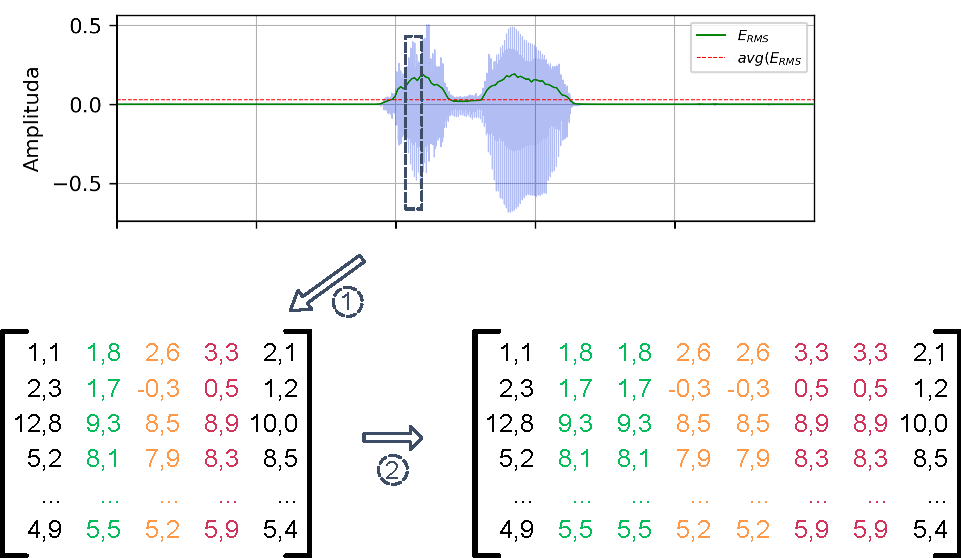
\includegraphics[width=0.9\textwidth]{./ch4-experiments/img/augmentation_features.pdf}
  \caption{Princip protažení na příznacích.}
  \label{fig:experiments:augmentation:features}
\end{figure}

Protažení na příznacích je, ale spíše hypotetická možnost. V reálné situaci by totiž řečník mluvil jako doposud a k protažení by docházelo při zpracování. Což je velmi netriviální úkol. Teoreticky by se musel v rámci parametrizace doplnit mechanismus, který by určité příznakové vektory určitým způsobem duplikoval. Navíc prosté zkopírování porušuje dynamický charakter řeči. V rámci jednoho zpracovávaného okénka (jednoho vektoru) jsou parametry považovány za statické, ale jak se okénko v rámci zpracování posouvá, tak už nelze hovořit o stacionaritě parametrů. Tento problém by se musel řešit nějakým druhem interpolace mezi dvěma konsekutivními vektory. Mechanismus by zároveň vyřešil omezení, kdy je kopírováním možné získat pouze protažení odpovídající celočíselnému násobku původní délky. Proč tedy vůbec zkoušet tento typ protažení? Odpověď je jednoduchá, nehraje zde takovou roli přesnost zarovnání. V průběhu zpracování je využíváno posuvného okénka a překryvu. Díky tomu dojde k určitému \uv{rozmazání} hranic. Pro úplně prvotní experimenty je to pak relativně vítané zjednodušení úlohy.

\subsubsection{Dosažené výsledky}

Prvním bodem výše zmíněného algoritmu je získání standardního modelu, který je použit k zarovnání dat. K tomu je možné použít již natrénovaný model z části \ref{chap:experiments:normalization:quality}. Jde tedy o \textit{HMM-DNN} model s $5$ skrytými vrstvami, každá s $4096$ neurony. Výstupní vrstva je pak typu softmax dimenze rovné počtu HMM stavů. Tento model dosáhl s monofónovým zerogramovým LM přesnoti $84,66\ \%$. S jeho pomocí je získáno zarovnání, tedy hranice jednotlivých fónému v trénovací i testovací sadě. Díky zarovnání je možné protáhnout zájmové fonémy.

V rámci testování celého procesu je jako prvotní ověřovací experiment zvoleno dvojnásoné protažení fonému $/s/$. Jinými slovy, všechny vektory odpovídající $/s/$ jsou zduplikovány. Následně je standardním způsobem natrénován \textit{HMM-DNN} model. Neuronová síť má tedy $5$ skrytých vrstev s $4096$. Výstupní vrstva je typu softmax. Otestování je pak jako v předchozích případech realizováno na testovací sadě s monofónovým zerogramovým jazykovým modelem. Tento nový model dosáhl přesnosti $85,11\ \%$, což je sice malé, ale přesto zlepšení.

Protažení $/s/$ posloužilo hlavně k ověření procesu vytváření modelu. Další experiment je realizován na protažených fonémech $/k/$, $/p/$, $/s/$, $/t/$ a $/v/$, což představuje většinu neznělých zájmových fonémů. Zarovnání je identické jako u předchozího experimentu, protože původní data se nezměnila. Opět je uvažováno dvojnásobné protažení. Všechny vektory inkriminovaných fonémů jsou zduplikovány. Znovu je natrénován \textit{HMM-DNN} model a otestován společně s monofonovým zerogramovým jazykovým modelem. Přesnost na testovací sadě dosáhla hodnoty $87,50\ \%$, což lze považovat za významné zlepšení.

Doposud se uvažovalo pouze o dvojnásobném protažení, v další fázi je tedy potřeba oveřit jestli jiné hodnoty nemohou poskytnout ještě lepší výsledek. Celkem je uvožované $3x$, $4x$ a $5x$ protažení. Uvažovány jsou fonémy $/k/$, $/p/$, $/s/$, $/t/$ a $/v/$. Proces natrénování a otestování modelu je stejný jako v předchozích případech. Dosažené výsledky jsou pak v tab. \ref{tab:experiments:augmentation:influence}. Pro úplnost je tabulka doplněna o baseline model s $1x$ protažením (tedy žádným) a již prezentované $2x$ protažení. Z výsledků je patrný jasný trend, větší než $2x$ protažení nemá smysl, protože se přesnost zhoršuje. Optimální hodnota protažení teoreticky leží někde v intervalu $\left(1,\ 3\right)x$, ale s protahovaním pomocí kopírování příznakových vektorů není možné přesné určení hodnoty.

\begin{table}[htpb]
  \centering
  \def\arraystretch{1.5}
  \pgfplotstabletypeset[
    col sep=semicolon,
    string type,
    columns/extension/.style={column name=, column type={|l}},
    columns/1x/.style={column name=1x, column type={|r}},
    columns/2x/.style={column name=2x, column type={|r}},
    columns/3x/.style={column name=3x, column type={|r}},
    columns/4x/.style={column name=4x, column type={|r}},
    columns/5x/.style={column name=5x, column type={|r|}},
    every head row/.style={after row=\hline, before row=\hline},
    every last row/.style={after row=\hline},
  ]{./ch4-experiments/tabs/0301-features.csv}
  \caption{Vliv míry protažení na přesnost modelu.}
  \label{tab:experiments:augmentation:influence}
\end{table}

Zhoršení přesnosti dozajista souvísí s faktem, že výsledná augmentovaná data neodpovídají realitě. Čím vícekrat je vektor zkopírován, tím více je vnášena chyba způsobená ignorováním dynamické povahy signálu. Nicméně jako proof-of-concept myšlenky posloužil tento experiment velmi dobře. Protažení na příznacích vede ke zvýšení přesnosti a má smysl tuto cestu více prozkoumat.

\subsection{Protažení na zvuku}
\label{chap:experiments:augmentation:audio}

\begin{itemize}
  \item problém se znělostí (systém moc nefunguje pokud je promluva krátká)
  \item popsat důvody pro protažení
  \item popis a výsledky experimentů na uměle protažených datech na příznacích (není použitelné reálně)
  \item aktualizace experimentu \uv{člověk vs. stroj}
\end{itemize}

% !TEX root = ../thesis.tex
\section{Model akcentující protažení dat}
\label{chap:realisation:durationmodels}

Augmentace dat (viz část \ref{chap:realisation:augmentation}) ukázala, že ztracenou informaci EL řeči je částečné možné nahradit protažením inkriminovaných fonémů. Experimenty s reálně protaženými daty (viz část \ref{chap:realisation:augmentation:real}) navíc prokázaly schopnost člověla toto protažení realizovat. Dalším krokem je tedy úprava modelu tak, aby tuto změnu co možná nejvíce reflektoval.

Z principu fungování a nejpoužívanější topologie HMM modelu (viz \ref{chap:asr:acoustic:HMM}) je délka fonému modelována pomocí přechodových pravděpodobností. Ty zase vedou na funkce geometrické distribuce pravděpodobnosti \cite{Rabiner1989}. Bohužel skutečná podoba těchto distribucí odpovídá spíše gamma nebo logaritmicko-normálnímu rozdělení \cite{Alumae2014}.

Správné modelování délky může být realizováno úpravou přechodových hustotních funkcí v HMM nebo změnou topologie modelu. Druhou možností je vytvoření speciálního modelu pracujícího s délkou jednotlivých fonémů (duration model) a reskórováním výstupních N-best hypotéz či celé rozpoznávací mřížky.

Přestože se první uvažovaný způsob jeví jako vhodnější, tak všechny dosavadní publikované výsledky ukazují významné zvýšení výpočetní náročnosti dekódování a komplexity modelu \cite{Rabiner1989} \cite{Pylkkonen2004} \cite{Russell1985}. Tento přístup je však často používán u HMM syntézy řeči, viz \cite{Yoshimura1998}.

\subsection{Princip explicitních duration modelů}
\label{chap:realisation:durationmodels:model}

Druhou možností je vytvoření explicitního modelu pracujícího s délkou fonémů. S tímto modelem je často problém rozpoznávání přeformulován do úlohy nalezení nejlepší sekvence slov $W^{*}$ a odpovídajících délek $D^{*}$, na základě akustického modelu \cite{Alumae2014}. Za předpokladu, že je dána sekvence slov $W$ a vektory pozorování $\boldsymbol{O}$ lze považovat za nezávislé na délkách $D$, je možné rovnici \ref{eq:asr:decoding} upravit jako

\begin{align}
  W^{*}, D^{*} &= \argmax_{W, D} P\left(W, D| O\right) \nonumber  \\
          &= \argmax_{W, D} P\left(O, D| W\right)P\left(W\right) \nonumber  \\
          &= \argmax_{W, D} P\left(O|W\right)P\left(D|W\right)P\left(W\right).
  \label{eq:realisation:durationmodels:assumtion}
\end{align}

\noindent Úkolem duration modelu je tedy odhad pravděpodobnosti $P\left(D|W\right)$. Délku $D$ je možné dekomponovat na $m$ délek jednotlivých fonémů $d_{i}$

\begin{equation}
  P\left(D | W\right) = P\left(d_{1}, \dots, d_{m}|W\right).
  \label{eq:realisation:durationmodels:decomposition}
\end{equation}

\noindent Tuto pravděpodobnost je dále možné upravit pomocí tzv. chain pravidla do tvaru

\begin{align}
  P\left(d_{1}, \dots, d_{m} | W\right) &= \prod_{i=1}^{m} P\left(d_{i} | d_{1}, \dots, d_{i-1}, W\right) \nonumber \\
        &\approx \prod_{i=1}^{m} P\left(d_{i} | d_{i-n-1}, \dots, d_{i-1}, W\right).
  \label{eq:realisation:durationmodels:chain}
\end{align}

\noindent Model tedy odhaduje $P\left(D|W\right)$ na základě $n$ předchozích délek fonémů a předpokládaného slova $W$. Některé duration modely navíc ještě pracují i s tempem řeči \cite{Pylkkonen2004}, nicméně tento efekt je u modelu využívající rovnici \ref{eq:realisation:durationmodels:chain} zakomponován v délkách $n$ předchozích fonémů.

Ve skutečnosti je vhodné vytvořit model, který bere v potaz nejen předchozí délky, ale i příznakové vektory těchto fonémů \cite{Alumae2014}. Tedy $P\left(d_{i}|x_{i}\right)$, kde $x_{i}$ představuje příznakový vektor obsahující délky $n$ předchozích fonémů, jejich vektory pozorování a případně další hodnoty. K odhadu této pravděpodobnosti se jako vhodné ukázaly neuronové sítě. \cite{Alumae2014} \cite{Hadian2017}

Na odhad $P\left(d_{i}|x_{i}\right)$ je možné nahlížet ze dvou pohledů. V prvním případě je cílem modelu odhadnout parametry pravděpobnostní distribuce pomocí conditional density estimation network (CDEN). \cite{Alumae2014} V tomto případě je předpokládáno, že délky fonémů odpovídají určitému pravděpodobnostnímu rozdělení, nejčastěji logaritmicko-normálnímu. Konkrétní hodnota pravděpodobnosti je pak vypočtena dosazením do příslušného vzorce hustoty pravděpodobnosti.

Druhou možností je stejně jako v případě HMM-DNN akustického modelu odhad pseudo-pravděpodobností za pomocí NN mající jako poslední vrstvu tzv. softmax vrstvu. Tento přístup nevnáší do modelu žádné předpoklady o podobě pravděpodobnostního rozdělení. Experimenty v \cite{Hadian2017} ukazují, že tento přístup je vhodnější\footnote{Při vytváření duration modelu byly otestovány oba přístupy a i naše experimenty ukazují, že NN se softmax vrstvou poskytuje lepší výsledky, protože u EL řeči CDEN model přinesl zanedbatelné zlepšení a v některých případech dokonce reskórování způsobilo zhoršení výsledků.}.

\subsection{Duration model se softmax vrstvou}
\label{chap:realisation:durationmodels:nn:softmax}

Neuronová síť mající na svém výstupu softmax vrstvu (viz rovnice \ref{eq:asr:acoustic:dnn:asr:softmax}) určuje diskrétní pseudo-pravděpodobnosti $m$ tříd. V případě duration modelu, se jako vhodné jeví reprezentovat jednotlivé třídy jako počet mikrosegmentů ($d=1,2,3,\dots$), které odpovídají danému fonému. Čistě teoreticky může být těchto mikrosegmentů nekonečné množství, síť však na svém výstupu potřebuje konečný počet tříd (počet neuronů ve výstupní vrstvě). Jako vhodné řešení tohoto problému se ukázalo zvolení maximální délky fonému $D$. Pro všechny s délkou $d \geq D$ platí, že $p\left(d\right) = p\left(D\right)$. \cite{Hadian2017} Volba $D$ závisí na konkrétní doméně a je vhodné ji určit experimentem.

Cílem modelu je predikovat sekvenci délek na základě sekvence fonémů. To implikuje možnost použití levého $L$ i pravého $R$ kontextu fonému $i$. Do vstupního vektoru sítě, ale mohou přijít délky pouze fonémů $L$ nebo $R$ kontextu. Pokud by totiž byly použity oba kontexty, tak by délka fonému $i$ závisela na délce fonému $i+1$. Zároveň by, ale délka fonému $i+1$ závisela na délce fonému $i$. Tím pádem by došlo ke kruhové závislosti, kterou není možné vyřešit. Standardně se volí $L$ kontext pro délky. Příznakový vektor tedy obsahuje následující položky:

\begin{itemize}
  \item Pro každý foném kontextu $-L \leq i \leq R$ je použito kódování 1 z n (1 pro správný foném, 0 pro ostatní, angl. one-hot encoding). Celková dimenze kontextu je tak $N_{p} \times \left(L + R + 1\right)$, kde $N_{p}$ je počet fonémů ve slovníku.
  \item Druhou množinu příznaků reprezentují otázky použité u fonetických rozhodovacích stromů (viz část \ref{chap:construction:results:reduction}). U těchto otázek je opět použito one-hot encoding. Dimenze těchto příznaků je $N_{q} \times \left(L + R + 1\right)$, kde $N_{q}$ odpovídá celkovému počtu otázek.
  \item Poslední skupinu příznaků představují délky fonémů L kontextu na pozicích $-L \leq i < 0$. Celková dimenze je $L$. Neuronová síť nejlépe pracuje s hodnotami v intervalu $\left(0, 1\right)$. Jako vhodné se ukázalo normalizovat hodnotu délky $d=1, 2, \dots, D$ pomocí sigmoid funkce

  \begin{equation}
    d^{\prime} = \frac{2}{1 + e^{-0,01d}} - 1,
    \label{eq:realisation:durationmodels:nn:normalization}
  \end{equation}

  \noindent která transformuje hodnoty do požadovaného intervalu $\left(0, 1\right)$ \cite{Alumae2014}. Pokud není kontext k dispozici (krajní případy), tak $d = 0$.
\end{itemize}

\noindent Celková dimenze výsledného příznakového vektoru je pak $I = \left(L + R + 1\right) \ast \left(N_{p} + N_{q}\right) + L$.

Samotné reskórování výstupní mřížky je realizováno přidáním $\log p\left(d_{i}| x_{i}\right)$, kde $x_{i}$ je vstupní příznakový vektor duration modelu, k hodnotám získaným z akustického a jazykového modelu. Mřížka je mezivýsledek, ze kterého je následně vydekódován výstup ASR systému. Samotné duration skóre je navíc přenásobeno konstantou získanou z development sady v průběhu trénování modelu tak, aby jeho řád odpovídal hodnotám z ostatních modelů. \cite{Hadian2017} Stejně jako v případě jazykového modelu je i zde tzv. váha duration modelu, která umožňuje měnit vliv tohoto modelu.

\subsection{Dosažené výsledky}
\label{chap:realisation:durationmodels:nn:softmax:results}

Stejně jako v případě augmentace dat (viz \ref{chap:realisation:augmentation:audio}) je potřeba k natrénování duration modelu kvalitní zarovnání. Jedním z hlavních částí příznakového vektoru modelu je totiž délka L kontextu modelu. K získání co možná nejpřesnějšího zarovnání je použit nejlepší TDNN model natrénovaný na uměle protažených datech\footnote{Natrénování TDNN modelu pomocí reálně protažených dat nebylo vhodné, protože nebylo k dispozici dostatečné množství reálně protažených dat.}, viz tab. \ref{tab:realisation:augmentation:influence:tdnn}.

Samotný duration model (popsaný v předchozí části \ref{chap:realisation:durationmodels:nn:softmax}) je typu feedforward.  Počet skrytých vrstev sítě se odvíjí od konkrétní řešené domény, ale standardně se uvažují $2$ případně $3$, viz \cite{Hadian2017}. Velikost těchto skrytých vrstev je volena jako násobek dimenze příznakového vektoru, v tomto případě byl zvolena hodnota $3I$. Aktivační funkce je typu RELU. Velikost výstupní vrstvy odpovídá maximálnímu počtu mikrosegmentů $D$, v \cite{Hadian2017} bylo dosaženo nejlepších výsledků s $D=50$. K vytvoření duration modelu posloužil framework Kaldi. Ten představuje obecný framework pro vytváření HMM a DNN řečových modelů.

Ověření funkčnosti duration modelu je provedeno na $2x$ uměle protažených datech\footnote{Hodnota $2x$ je zvolena, protože se nejvíce blíží reálně protaženým datům.}. Kontextuální okénko má hodnotu $\left(L, R\right) = \left(3, 3\right)$, $N_{p} = 42$ a $N_{q} = 6$. Velikost vstupního vektoru $I = 339$. Model má $2$ skryté vrstvy o velikosti $1017$ neuronů. Výstupní vrstva typu softmax má dimenzi $D=50$. Model je trénován a otestován pomocí stejné trénovací a testovací sady jako modely v části \ref{chap:realisation:augmentation:audio}. Jazykový model je fonémový zerogramový. Tento model dosáhl $Acc_{p} = 88,54\ \%$, což představuje zlepšení o $0,83\ \%$ absolutně a $7,24\ \%$ relativně oproti TDNN $2x$ modelu ($Acc_{p} = 87,71\ \%$). Duration model tedy relativně významně zlepšuje přesnost modelu. Na reálně protažených datech pak tento model dosáhl přesnosti $Acc_{p} = 85,68\ \%$ (původní TDNN $2x$ model dosáhl $Acc_{p} = 84,51\ \%$). Pokud vstupem duration modelu byla neprotažená data, tak přesnost modelu byla pouze $Acc_{p} = 80,73\ \%$. Z analýzy chyb pak plyne, že v takovém případě významně přibylo chyb u vybraných neznělých fonémů. Tento výsledek, ale přesně kopíruje očekávání, protože je model natrénován na protaženou podobu.

Mezi hyperparametry modelu patří zejména velikost $L$ a $R$ kontextu, počet vrstev sítě a maximální délka $D$. Zejména hodnota maximální délka $D$ teoreticky poskytuje největší možnost pro zlepšení výsledků modelu, protože hodnota $D=50$ byla zvolena na základě experimentů provedených v \cite{Hadian2017}, kde se však pracovalo se standardní neprotaženou řečí. Tab. \ref{tab:realisation:duration:duration} ukazuje vliv maximální délky na přesnost modelu. Speciální je hodnota $D=189$, která je určena automaticky na základě zarovnání před samotným trénováním. Model s $D=189$ zároveň dosáhl nejvyšší přesnosti $Acc_{p} = 88,58\ \%$, což představuje drobné zlepšení oproti původnímu modelu s $D = 50$.

\begin{table}[htpb]
  \centering
  \def\arraystretch{1.5}
  \pgfplotstabletypeset[
    col sep=semicolon,
    string type,
    columns/header/.style={
      column name={},
      column type={l},
      string replace={accp}{$Acc_{p}\ [\%]$}
    },
    columns/50/.style={column name={50}, column type={r}},
    columns/100/.style={column name={100}, column type={r}},
    columns/150/.style={column name={150}, column type={r}},
    columns/189/.style={column name={189}, column type={r}},
    columns/200/.style={column name={200}, column type={r}},
    every head row/.style={
      before row={\toprule & \multicolumn{5}{c}{D} \\},
      after row={\midrule}
    },
    every last row/.style={after row={\bottomrule}}
  ]{./ch6-realisation/tabs/01-duration_value.csv}
  \caption{Vliv maximální délky na přesnosti modelu.}
  \label{tab:realisation:duration:duration}
\end{table}

Dalším hyperparametrem, který může ovlivnit kvalitu modelu je počet vrstev neuronové sítě. V tab. \ref{tab:realisation:duration:layers} jsou vypsány výsledky jednotlivých modelů. Varianta \textit{1H} představuje model s $1$ skrytou vrstvou, \textit{2H} model s $2$ skrytými vrstvami a \textit{3H} s $3$ skrytými vrstvami. Speciálním případem jsou modely obsahující bottleneck vrstvu (\textit{2H (bottleneck)} a \textit{3H (bottleneck)}). Ty místo poslední skryté vrstvy o velikosti $3I$ obsahují vrstvu s pouze $10$ neurony. Tato vrstva by měla pomoci v zobecňování \cite{Hadian2017}. Z dosažených výsledků je patrné, že velikost sítě není úplně zásadním parametrem. Rozdíl mezí přesností sítě s $2$ a $3$ vrstvami je minimální. Přínos bottleneck vrstvy, oproti výsledkům prezentovaným v \cite{Hadian2017}, je také spíše minimální. Nicméně obecně se dá říci, že tato vrstva má pozitivní dopad na přesnost.

\begin{table}[htpb]
  \centering
  \def\arraystretch{1.5}
  \pgfplotstabletypeset[
    col sep=semicolon,
    string type,
    columns/layers/.style={
      column name={},
      column type={l},
      string replace={accp}{$Acc_{p}\ [\%]$}
    },
    columns/1H/.style={column name={1H}, column type={r}},
    columns/2H/.style={column name={2H}, column type={r}},
    columns/3H/.style={column name={3H}, column type={r}},
    columns/2Hb/.style={column name={2H (bottleneck)}, column type={r}},
    columns/3Hb/.style={column name={3H (bottleneck)}, column type={r}},
    every head row/.style={
      before row={\toprule & \multicolumn{5}{c}{Model} \\},
      after row={
        % \cmidrule{2-6}
        \midrule
      }
    },
    every last row/.style={after row={\bottomrule}},
  ]{./ch6-realisation/tabs/02-layers.csv}
  \caption[Vliv počtu vrstev]{Vliv počtu skrytých vrstev na přesnosti modelu ($D = 189$\footnotemark).}
  \label{tab:realisation:duration:layers}
\end{table}

\footnotetext{V průběhu určování nejlepších kombinace hyperparametrů byly otestovány všechny kombinace velikosti sítě a maximální délky $D$. Nejlepších výsledků dosahovaly modely s $D=189$.}

Posledním hyperparametrem, který může mít vliv na přesnost modelu je velikost $L$ a $R$ kontextu. Z tab. \ref{tab:realisation:duration:context:symetric} a tab. \ref{tab:realisation:duration:context:asymetric} vyplývá, že nejlepších výsledků dosahuje modely, který má délku kontext $L + R = 6$. Úplně nejlepšího výsledku pak dosáhl model mající symetrický kontext, ale oproti modelům s asymetrickým kontextem je rozdíl spíše zanedbatelný.

\begin{table}[htpb]
  \centering
  \def\arraystretch{1.5}
  \pgfplotstabletypeset[
    col sep=semicolon,
    string type,
    columns/context/.style={
      column name={},
      column type={l},
      string replace={accp}{$Acc_{p}\ [\%]$}
    },
    columns/0/.style={column name={(0, 0)}, column type={r}},
    columns/1/.style={column name={(1, 1)}, column type={r}},
    columns/2/.style={column name={(2, 2)}, column type={r}},
    columns/3/.style={column name={(3, 3)}, column type={r}},
    columns/4/.style={column name={(4, 4)}, column type={r}},
    every head row/.style={
      before row={\toprule & \multicolumn{5}{c}{Kontext \textit{(L, R)}} \\},
      after row={
        % \cmidrule(r){1-1}
        % \cmidrule{2-6}
        \midrule
      }
    },
    every last row/.style={after row={\bottomrule}},
  ]{./ch6-realisation/tabs/03-context.csv}
  \caption{Porovnání vlivu velikosti symetrického kontextu.}
  \label{tab:realisation:duration:context:symetric}
\end{table}

\begin{table}[htpb]
  \centering
  \def\arraystretch{1.5}
  \pgfplotstabletypeset[
    col sep=semicolon,
    string type,
    columns/context/.style={
      column name={},
      column type={l},
      string replace={accp}{$Acc_{p}\ [\%]$}
    },
    columns/5/.style={column name={(5, 1)}, column type={r}},
    columns/4/.style={column name={(4, 2)}, column type={r}},
    columns/3/.style={column name={(3, 3)}, column type={r}},
    columns/2/.style={column name={(2, 4)}, column type={r}},
    columns/1/.style={column name={(1, 5)}, column type={r}},
    every head row/.style={
      before row={\toprule & \multicolumn{5}{c}{Kontext \textit{(L, R)}} \\},
      after row={
        % \cmidrule(r){1-1}
        % \cmidrule{2-6}
        \midrule
      }
    },
    every last row/.style={after row={\bottomrule}},
  ]{./ch6-realisation/tabs/04-context.csv}
  \caption{Vliv levého a pravého kontextu v případě, že celková délka $L + R = 6$.}
  \label{tab:realisation:duration:context:asymetric}
\end{table}

Nejlepšího výsledku tedy dosahuje model mající $D = 189$, $2$ skryté vrstvy, kde poslední skrytá vrstva má pouze $10$ neuronů a $L + R = 6$. Výsledky však ukazují, že duration model není významně citlivý na změnu parametrů. V případě rozpoznávání reálně protažených dat, dosáhl model přesnosti $Acc_{p} = 85,93\ \%$. Pokud se trénovací sada modelu rozšířila o část reálně protažených dat ($10\ \%$ a $25\ \%$ vět) a natrénoval a otestoval se nový model (pomocí zbytku reálně protažených dat), tak výsledná přesnost dosáhla hodnoty $Acc_{p} = 87,02\ \%$. Hodnoty přesnosti však nejsou úplně porovnatelné, protože testovací sada není identická, nicméně lze vyvozovat závěr, že pokud by byl model natrénován z dostatečného množství reálně protažených dat, tak by se jeho výsledky blížily výsledkům modelu na uměle protažených datech.


\subsection{Aktualizace výsledků porovnání}
\label{chap:realisation:duration:comparison}

V části \ref{chap:realisation:listening} a \ref{chap:realisation:augmentation:comparison} jsou prezentovány výsledky srovnání schopností člověka a stroje. V případě člověka jsou zdrojem dva poslechové testy, které prověřily schopnost posluchače nejprve určit význam izolovaných slov a následně od sebe rozeznat dvě akusticky velmi podobná slova. V případě stroje jsou použity celkem $3$ ASR experimenty \uv{one-mil}, \uv{reduced} a \uv{bigrams}. V tab. \ref{tab:realisation:duration:comparison} jsou pak předchozí výsledky doplněny o hodnoty dosažené duration modelem jehož parametry odpovídají nejlepšímu modelu z předchozí části \ref{chap:realisation:durationmodels:nn:softmax}.

Stejně jako v předchozích experimentech je u \uv{one-mil} experimentu použit zerogramový jazykový model s 1 milionem slov, \uv{reduced} obsahuje pouze slova obsažená v poslechovém testu. V případě \uv{bigrams} je pro každou položku generován speciální LM obsahující 4 kombinace slov. Použití duration modelu nepřineslo významné zlepšení výsledků \textit{augmented} modelu. Tento výsledek, ale není překvapivý, protože \textit{augmented} model dosahuje teoreticky maximálních možných hodnot. Největšího zlepšení dosáhl duration model v případě \uv{one-mil} experimentu. Zde došlo ke zlepšení o $1,42\ \%$ absolutně, což je o $10,42\ \%$ relativně. Rozhodně se jedná o významné zlepšení.

\begin{table}[htpb]
  \centering
  \def\arraystretch{1.5}
  \pgfplotstabletypeset[
    col sep=semicolon,
    string type,
    columns/type/.style={column name=, column type={l}},
    columns/onemil/.style={column name={one-mil}, column type={r}},
    columns/reduced/.style={column name=reduced, column type={r}},
    columns/bigrams/.style={column name=bigrams, column type={r}},
    every head row/.style={
      after row={
        % \cmidrule(lr){1-1}
        % \cmidrule(lr){2-4}
        \midrule
      },
      before row={\toprule & \multicolumn{3}{c}{$Acc_{p}\ [\%]$} \\}
    },
    every last row/.style={
      after row={\bottomrule},
      before row={\midrule}
    },
  ]{./ch6-realisation/tabs/05-comparison.csv}
  \caption{Aktualizované porovnání dosažených výsledků člověka a stroje.}
  \label{tab:realisation:duration:comparison}
\end{table}

Použití reskóringu pomocí duration modelu ještě zlepšuje výsledky TDNN modelu natrénovaného na protažených datech. Oba modely navíc dokáží pracovat i s řečníkem reálně protaženými daty, což umožňuje i reálné použití těchto modelů. Hlavním nedostatkem aktuální implementace reskóringu pomocí duration modelu spočívá v tom, že se jedná o offline přístup. Promluvy jsou nejprve zpracována pomocí TDNN modelu a až následně jsou kompletní výstupy modelu reskórovány pomocí duration modelu. Změna modelu a principu reskórování tak, aby byl schopen pracovat i v online režimu je otázkou budoucího výzkumu, ale principiálně tomu nic nebrání.

% %!TEX root = ../thesis.tex
\section{Rehabilitace hlasu po totální laryngektomii}
\label{sec:cause:treatment}

Nesporná výhoda totální laryngektomie neoddiskutovatelně spočívá v likvidaci
primárního nádorového onemocnění. Následky operace však s sebou nesou obrovský
zásah do kvality života pacienta. Okem nejviditelnější změnu představuje
přítomnost tracheostomie a s ní spojený způsob dýchání. Tato skutečnost má
spoustu, na první pohled ne úplně očividných, následků. Postižený člověk
ztrácí přirozené zvlhčování, ohřev a filtraci vdechovaného vzduchu, jež má za
následek vyšší náchylnost k~respiračním onemocněním. Příčina spočívá v
průchodu vzduchu do průdušnice přes tracheostomii a nikoli přes nosní dutiny.

Pro samotného pacienta je však nejspíše nejobtížnější se vypořádat s trvalou
ztrátou vlastního hlasu. Z tohoto důvodu se již samotný autor procedury doktor
Billroth zaobíral otázkou rehabilitace hlasu. Jeho první pokusy s kovovou
tracheostomickou kanylou sice umožňovaly pacientovi hovořit, ale svou
konstrukcí pacienta spíše ohrožovaly na životě \cite{Kramp2009}. Proto se více
uchytila metoda tzv. jícnového hlasu \cite{Sebova-Sedenkova2006}. Ve stejnou
dobu, tedy přibližně začátkem minulého století, se začaly objevovat první
interní a externí hlasové aparáty. V současnosti je rehabilitace hlasu možná
pomocí:

\begin{itemize}
  \item \textbf{foniatrických metod}, mezi které patří jícnový hlas a elektrolarynx,
  \item \textbf{chirurgicko-protetickým způsobem}, který spočívá ve vytvoření kanálku skrze stěnu mezi průdušnicí a jícnem,
  \item \textbf{vytvoření hrtanu podobných struktur chirurgickým způsobem},
  \item \textbf{transplantace hrtanu}.
\end{itemize}

Z uvedeného výčtu se může zdát, že máme k dispozici relativně širokou škálu
možností, jak pacientovi vrátit schopnost vyjadřování pomocí mluvené řeči.
Ovšem je nutné si uvědomit, že je potřeba volit konkrétní metodu podle stavu a
možností pacienta. Jinými slovy, ne každá metoda se hodí pro každého pacienta
a žádná z~metod není univerzální pro všechny pacienty.

\subsection{Foniatrické metody} % (fold)
\label{sub:cause:treatment:foniatric}

Ačkoli odstranění hrtanu vyústí ve ztrátu hlasu, neznamená to, že by byla
úplně eliminována schopnost produkovat řeč. V procesu vytváření hlasu zastává
odstraněný orgán pouze (i když velmi zásadní) roli generátoru zvuku. Zbylé
orgány (hrdelní, nosní a ústní dutina a další) zůstávají nedotčeny a mohou i
nadále plnit svou funkci. Logicky se tak nabízí myšlenka nahradit chybějící
zdroj zvuku jiným. Mezi nejpoužívanější metody patří jícnový hlas a
elektrolarynx.

\subsubsection{Jícnový hlas} % (fold)
\label{ssub:cause:treatment:foniatric:esophageal}

Počátek této metody se datuje do roku 1922, kdy si prof. MUDr. Miloslav Seeman
\cite{seeman1922speech} uvědomil, že funkci štěrbiny mezi hlasivkami (rima
glottidis) přebírá tzv. pseudoglottis, která se vytváří na úrovni horního
jícnového svěrače. Zároveň vypracoval a popsal metodiku vytváření jícnového
hlasu, při které se vzduch neplní do plic, ale do jícnu. Tato metoda se nazývá
\textbf{aspirační}. Princip spočívá v aktivním otevření jícnového svěrače,
nasáváním a vtlačováním vzduchu do jícnu pomocí polykání. Naplněním jícnu
vzduchem si pacient připravuje potřebný vzduch k následné
eruktaci\footnote{eruktace - latinsky název pro proces říhání (popřípadě
krkání), při kterém dochází k úniku plynů pocházejících ze žaludku dutinou
ústní.} vzduchu a produkci řeči. Vlastní jícnový hlas poté vzniká na přechodu
jícnu a hypofaryngu (spodní část hltanu). V této oblasti horního jícnového
zúžení dochází k rozkmitání sliznice a podslizniční vrstvy a produkci zvuku,
který je následně modulován stejně jako v případě přirozené produkce řeči.
Princip tvorby \uv{základního} tónu jícnového hlasu je znázorněn na obr.
\ref{fig:cause:treatment:esophageal}.

\begin{figure}[htb]
  \begin{center}
    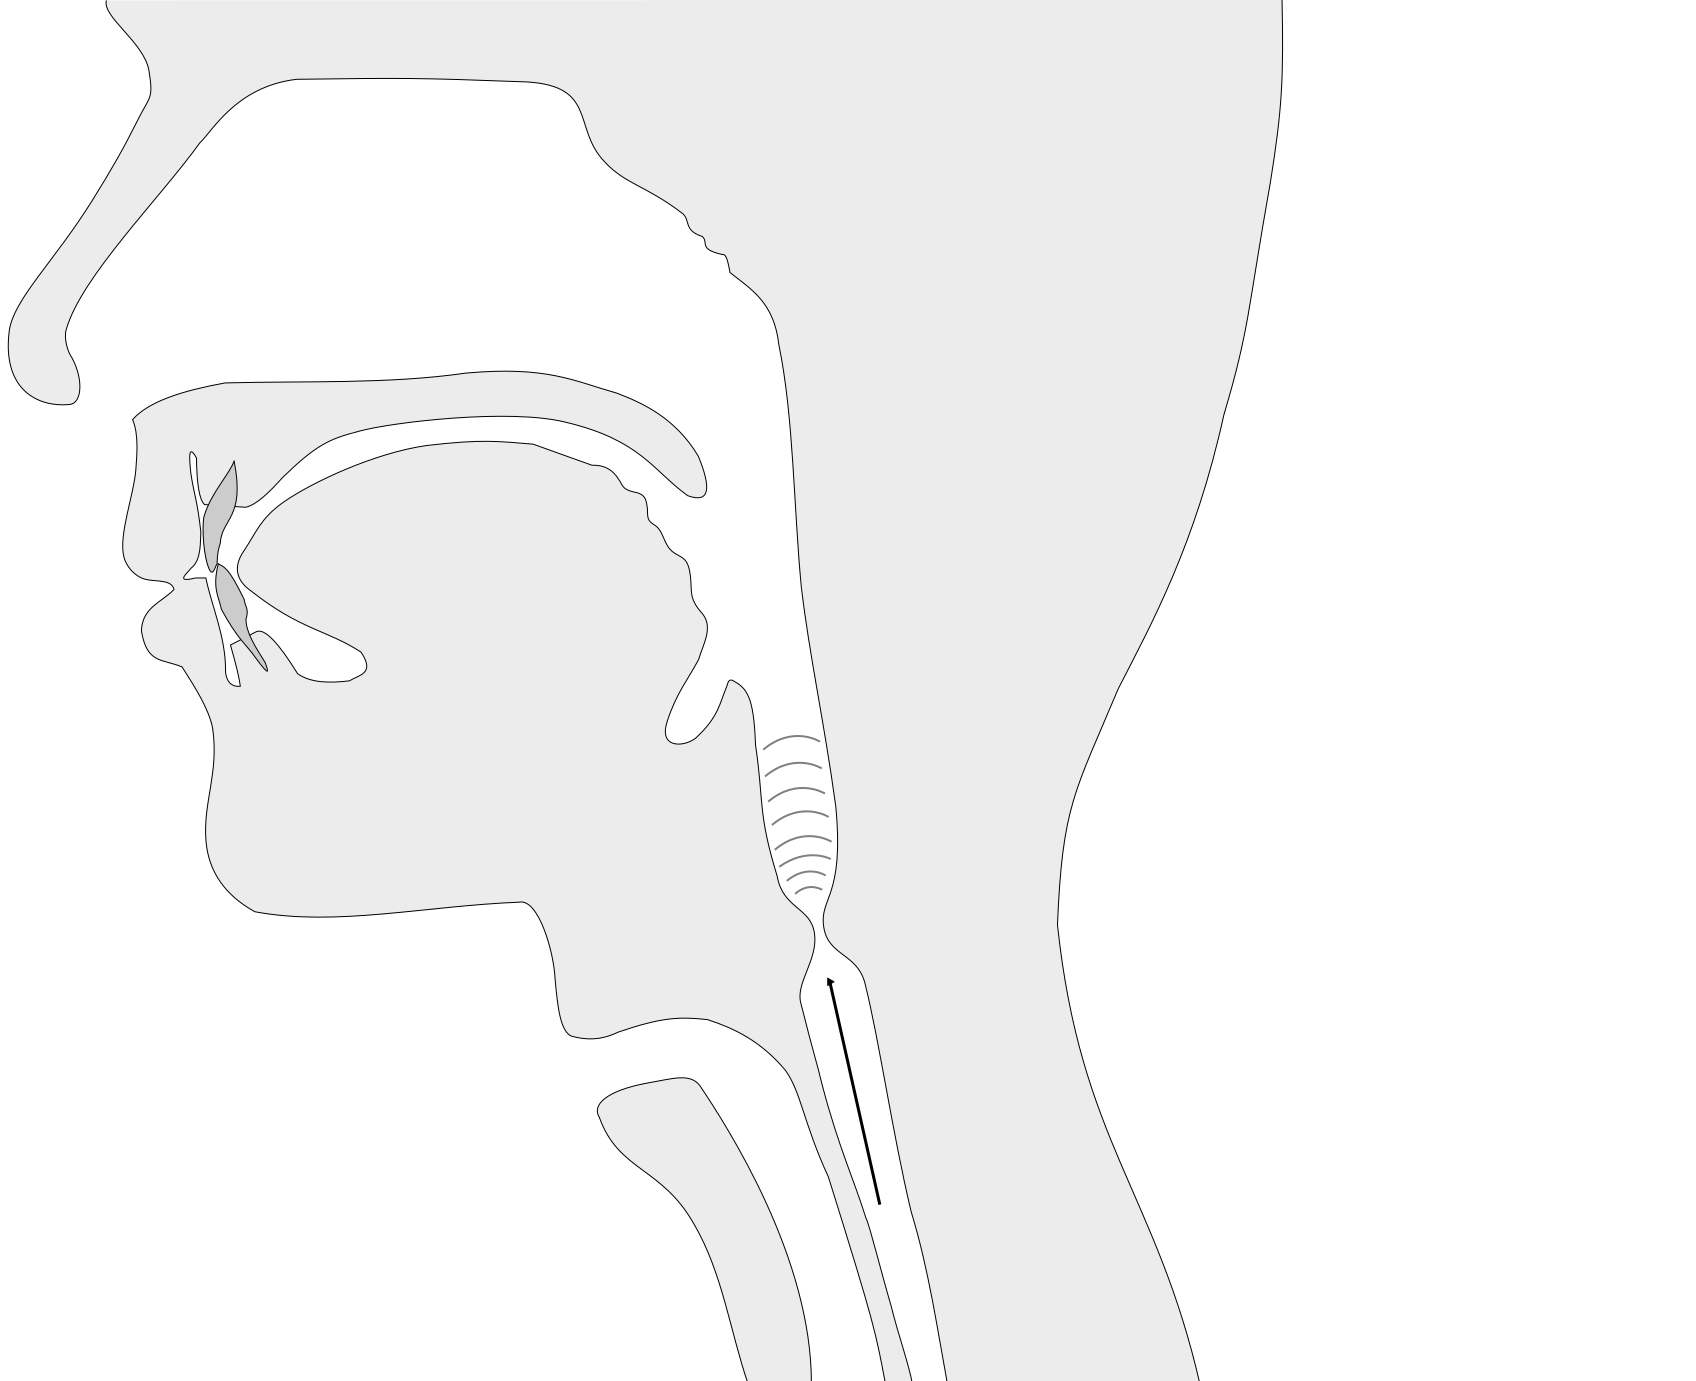
\includegraphics[width=0.6\linewidth]{ch2-cause/figures/esophageal}
    \caption[Princip tvorby jícnového hlasu]{Princip tvorby jícnového hlasu. Průchodem vzduchu přes zúžení vzniká základní tón jícnového hlasu.}
    \label{fig:cause:treatment:esophageal}
  \end{center}
\end{figure}

Kromě aspirační metody je ještě možné se setkat s metodou \textbf{injekční}.
Hlavní rozdíl spočívá v principu plnění vzduchu do jícnu. Při aspirační metodě
se využívá polykání, zatímco v tomto případě je využito kořene jazyka, kterým
je vzduch vtlačován do jícnu. Následný princip produkce hlasu je již shodný s
původní metodou. S tímto principem se můžeme setkat u pacientů, kterým byla
při laryngektomii odstraněna jazylka a aspirační náplň není možná.

Proces učení jícnového hlasu by měl začít co možná nejdříve po operaci. Pokud
je to možné, tak se s výukou začíná ještě za pobytu pacienta na ORL klinice
nebo krátce po propuštění. V první fázi se pacient učí pouze slabiky
sestávající z explosivy a souhlásky. Postupně se však přidávají slabičné
shluky, které sice nedávají smysl, ale pomáhají v osvojení potřebné techniky.
V případě úspěšného zvládnutí se přistupuje k nácviku frází a souvislé řeči.
Potřebnou dobu k nácviku jícnového hlasu nelze přesně určit, protože je
závislá na mnoha faktorech. V literatuře se uvádí, že je potřeba 30 až 50
hodin velmi intenzivního tréninku k osvojení jícnového hlasu.

Míra úspěšnosti nácviku srozumitelného hlasu se uvádí v rozsahu od 14\% do
75\%. Takto obrovský rozsah značí o mnoha faktorech, které mohou ovlivnit
úspěšné osvojení jícnového hlasu. Mezi možné příčiny neúspěchu patří
fyziologické nebo anatomické problémy, psychologické problémy, nebo jednoduše
neadekvátní podpora při řečové terapii \cite{Brown2003}. Velkou roli také
hraje snaha a odhodlání samotného pacienta.

Nepopíratelnou výhodou této techniky rehabilitace je nezávislost pacienta na
lékaři po úspěšném osvojení jícnového hlasu a permanentní oddělení dýchacích a
polykacích cest bez rizika vniknutí potravy do dýchacích cest. Mezi nesporné
výhody také patří volné ruce při vytváření řeči. Za nevýhody se obecně
považuje srozumitelnost produkovaného hlasu. Je to způsobeno jednak
\uv{břišním} zabarvením, které je už z podstaty metody přítomné, a dále také
nízkou intenzitou a krátkou výdrží při tvorbě tónu. Za negativum se dá také
považovat množství pacientem vynaloženého úsilí potřebného k osvojení
techniky. Velmi často se také mluvčí ostýchají jícnový hlas používat, protože
mají pocit, že je společensky nevhodné dorozumívat se formou blízkou říhání. Z
tohoto důvodu se odhaduje, že v běžném životě využívá jícnový hlas pouze 20 až
30\% pacientů, kteří se začali tuto techniku učit \cite{Hradecka2007}.

% subsubsection jícnový_hlas (end)

\subsubsection{Elektrolarynx} % (fold)
\label{ssub:cause:treatment:foniatric:elektrolarynx}

Rehabilitace hlasu pomocí elektrolarynxu se řadí mezi tzv. elektromechanické
metody. Princip spočívá v přikládání zařízení, které obsahuje generátor zvuku
nazývaný elektrolarynx. Přiložením do oblasti spodiny úst a aktivací zařízení
se generovaný zvuk a vibrace přenášejí do dutiny ústní a dalších přilehlých
artikulačních orgánů. Následnou artikulací je pacient schopen hovořit.
Znázorněno na obr. \ref{fig:cause:treatment:electrolarynx}.

\begin{figure}[htb]
  \begin{center}
    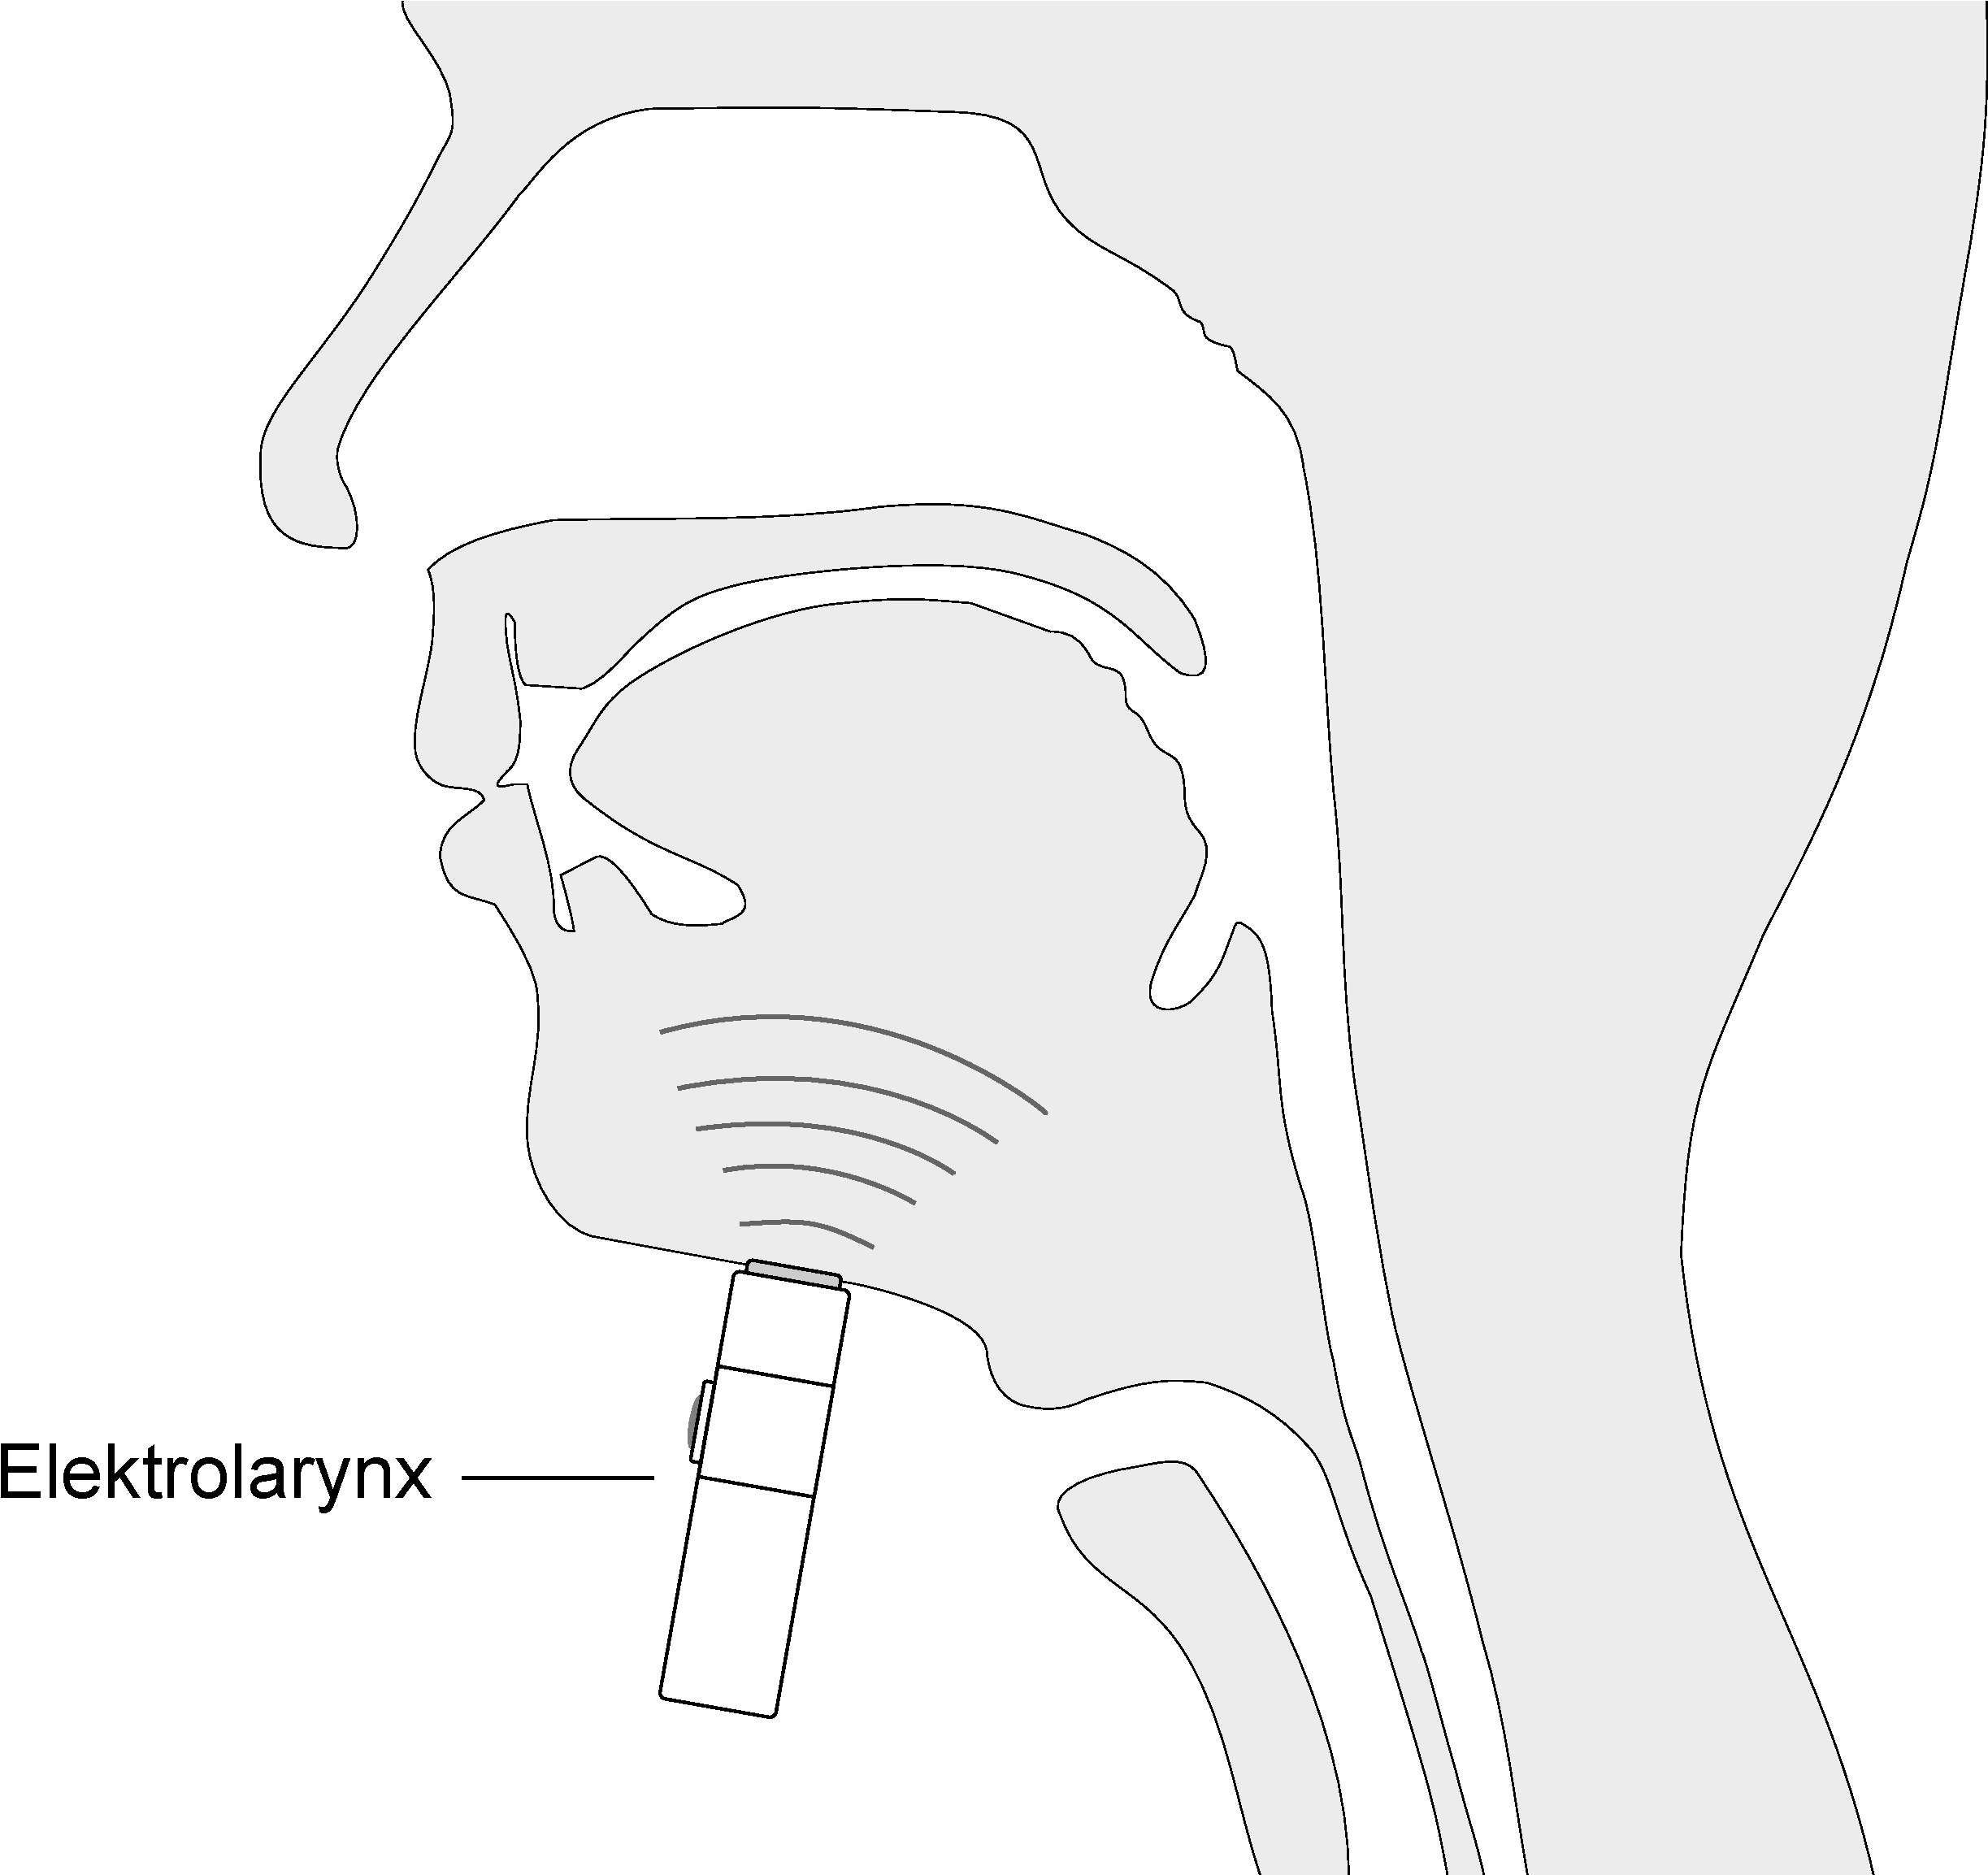
\includegraphics[width=0.6\linewidth]{ch2-cause/figures/electrolarynx}
    \caption[Princip rehabilitace hlasu pomocí elektrolarynxu]{Princip rehabilitace hlasu pomocí elektrolarynxu.}
    \label{fig:cause:treatment:electrolarynx}
  \end{center}
\end{figure}

% TODO: ELEKTROLARYNX pasaze o monotonosti reci poradne promyslet

Takto generovaná řeč se vyznačuje několika charakteristickými rysy. V první
řadě řeč budí velmi mechanický dojem. Důvodem je samozřejmě samotný
elektrolarynx, jelikož se jedná o elektromechanický generátor zvuku s
konstantním buzením, je také základní frekvence produkovaného hlasu více či
méně konstantní. Řečník tak má velmi omezené možnosti, jak řeč emotivně
zabarvovat. V průběhu času se objevily snahy průběžně měnit frekvenci zařízení
a tím ovlivňovat základní frekvenci produkované řeči \cite{Kikuchi2004,
Uemi1994, Goldstein2004}. Hlavním problém všech těchto zařízení je docílit
změnu fundamentální frekvence na základě toho, co chce řečník říci. V současné
době existují pouze experimentální zařízení, která umožňují ve velmi omezené
míře změnu frekvence \cite{Liu2007}. Další charakteristický rys představuje
nižší srozumitelnost řeči, která se ještě snižuje s~rostoucím okolním hlukem.
Velmi často se stává, že posluchač, který se s takto produkovanou řečí setkává
poprvé, není schopen plně porozumět. Se srozumitelností souvisí i další
charakteristický rys, kterým je přítomnost zvukového podkresu produkovaného
samotným přístrojem.

Za hlavní výhodu elektrolarynxu se považuje rychlost osvojení schopnosti
produkovat řeč. Zároveň je tato metoda vhodná pro téměř všechny pacienty
postižené ztrátou hlasu způsobenou léčbou karcinomu hrtanu. Z tohoto důvodu se
hojně užívá u pacientů, kteří si neosvojili jícnový hlas nebo u nich není
možné využití ostatních chirurgických metod.
Za nevýhody se obecně pokládá kvalita produkované řeči, tedy monotonní a
mechanicky znějící hlas. Dále potom zaměstnání jedné ruky držením nebo
spouštěním zařízení.

Samostatnou kapitolou může být psychologický dopad na pacienta. Stejně jako
u~jícnového hlasu se řeč produkovaná promocí elektrolarynxu jeví odlišně od
řeči přirozené. Navíc se ještě přidává potřeba využití nějakého zařízení.
Člověk proto v~mnoha případech cítí ostych a bojí se na veřejnosti mluvit.

% subsubsection elektrolarynx (end)

% subsection subsection_name (end)

\subsection{Chirurgicko-protetická metoda} % (fold)
\label{sub:cause:treatment:tracheo}

Další možnost rehabilitace hlasu představuje tracheoezofageální (zkr. TE) protéza.
První zmínka o vytvoření fistule\footnote{fistule (česky píštěl) je abnormální
otvor mezi dvěma dutými orgány, nebo mezi dutým orgánem a kůží.} mezi
průdušnicí a jícnem pochází z roku 1932. V~tomto roce doktor Guttman poprvé
vytvořil tracheoezofageání shunt\footnote{shunt - kanál, kterým je tekutina
odkloněna z přirozené dráhy. Tento kanál může být vytvořen chirurgicky nebo
pomocí syntetické trubice.} (\uv{umělá píštěl}). Hlavní myšlenka spočívá ve
vytvoření cesty prostřednictvím píštěle, pomocí které u tracheostomovaného
člověka může proudit vzduch z plic do úst. Za normálních okolností vzduch
proudí skrze tracheostomii a do úst se tak nedostane. Zacpe-li si pacient
stomu, může proud vzduchu proudit skrze píštěl do úst. Vzduch procházející
přes fistuli naráží do stěn jícnu a je rozvibrován. Tyto vibrace jsou následně
modulovány pomocí artikulačních ústrojí a tak vzniká řeč.
Tento ojedinělý zákrok otevřel cestu k chirurgické hlasové rehabilitaci.
Vzniklo několik operačních metod, které se navzájem lišili víceméně jen
umístěním fistule \cite{Kramp2009}.

Hlavní snahou chirurgů bylo vytvoření bezpečné, správně nasměrované píštěle
umožňující tvorbu hlasu. Bohužel v mnoha případech byly tyto zákroky spojené
s~vážnými komplikacemi (infekce, zápaly či těžká krvácení). Důležitým
problémem, se kterým se jednotlivý tvůrci museli vypořádat, byla stálost
vytvořeného otvoru tak, aby jím neprotékaly tekutiny špatným směrem a
nedocházelo k zatékání do dýchacích cest a orgánů. Jelikož se jednalo o velmi
náročné techniky, a bylo s nimi spojeno velké množství rizik, došlo v
80.letech 20.století k opadnutí snah tyto metody aplikovat.

Svou renesanci zažily s vložením jednocestného ventilu, který umožňoval pouze
jednosměrný průchod tekutin skrze píštěl, jak je ilustrováno na obr.
\ref{fig:cause:treatment:shunt}. První komerčně dostupná protéza se objevila
v~80.letech 20.století v USA. Na obr. \ref{fig:cause:treatment:prosthesis} jsou
zobrazeny příklady různých typů protéz. Na používané protézy jsou kladené
přísné nároky a musí vyhovovat určitým požadavkům. Předně se musí vyrábět
z~biokompatibilního materiálu, který odolává biodegradaci. Tím je zaručena
dlouhodobá trvanlivost a správná funkce. Potřebný tlak k otevření
faryngoezofageálního segmentu by měl být co nejnižší, aby bylo možné vytvářet
plynulou řeč. První vyráběné protézy měly tento tlak příliš vysoký a omezovaly
tak množinu potencionálních pacientů. Nejmodernější protézy se již vyznačují
velmi nízkým otevíracím fonačním tlakem. V~neposlední řadě by měla být protéza
samofixační a snadno vyměnitelná.

\begin{figure}[htb]
  \begin{center}
    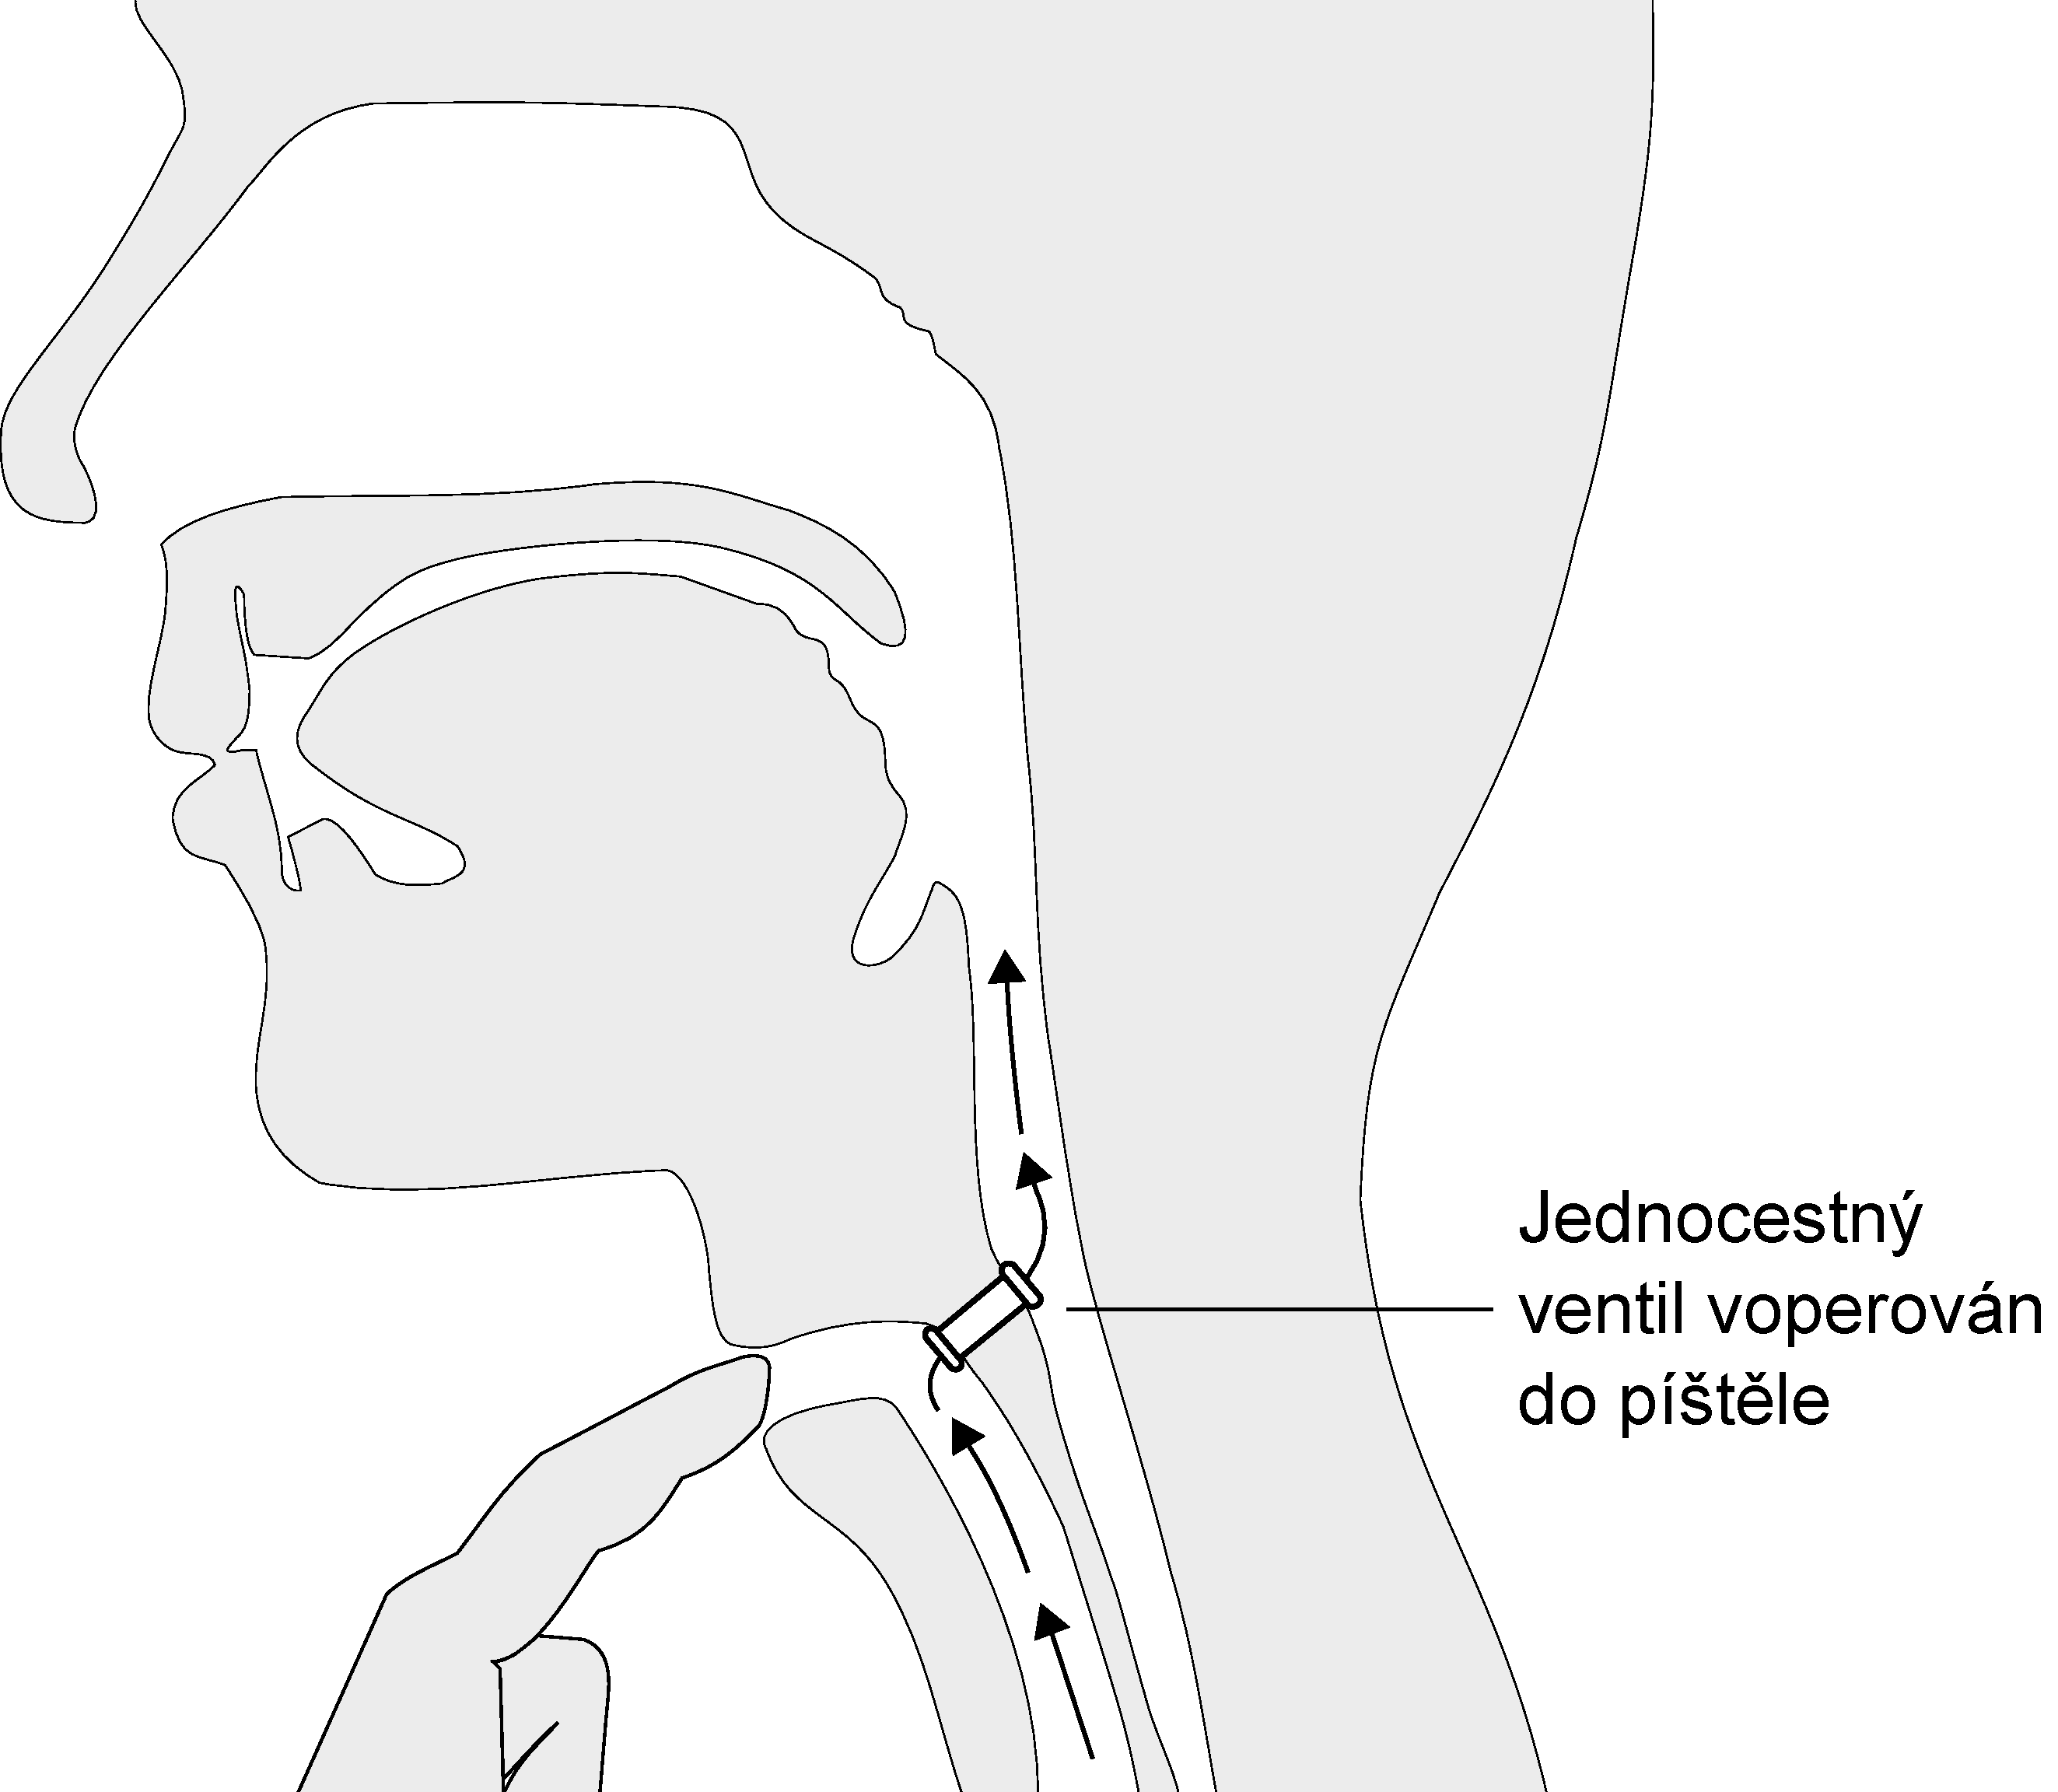
\includegraphics[width=0.6\linewidth]{ch2-cause/figures/te-shunt}
    \caption[Průchod vzduchu tracheoezofageální protézou]{Průchod vzduchu tracheoezofageální protézou.}
    \label{fig:cause:treatment:shunt}
  \end{center}
\end{figure}

\begin{figure}[htb]
  \begin{center}
    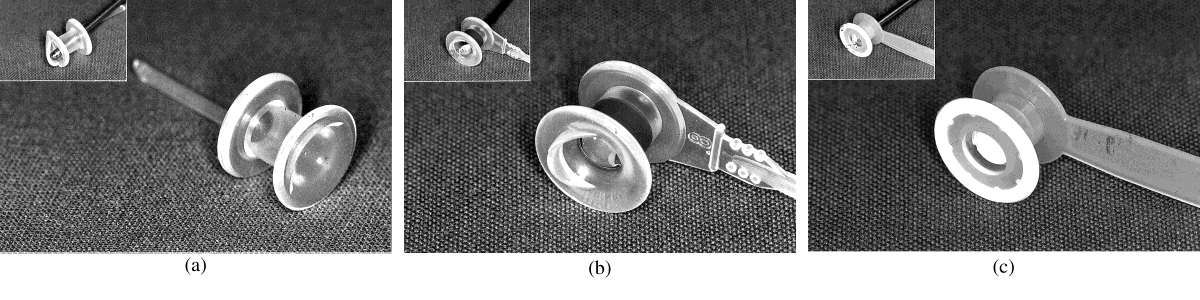
\includegraphics[width=0.9\linewidth]{ch2-cause/figures/te-protezy}
    \caption[Ilustrace používaných TE protéz]{Ilustrace používaných TE protéz (a) Gronigenova nízkotlaká protéza, (b) Provox2 a (c) Blom-Singer protéza.}
    \label{fig:cause:treatment:prosthesis}
  \end{center}
\end{figure}

V praxi se používá několik druhů protéz. Hlavním rozdílem mezi nimi však je
zda se pacient přímo účastní výměny ventilu, jehož fundamentální funkcí je
vytvoření průchodu pro vzduch proudící z průdušnice do jícnu. U protéz, které
jsou vyměňovány operačně, se doba používání pohybuje od 3 do 6 měsíců. Tento
interval velmi významně ovlivňuje tvorba biofilmu na povrchu náhrady. K tvorbě
dochází následkem přímého kontaktu protézy s tělními tekutinami a potravou.
Rychlost tvorby biofilmu ovlivňuje tvar a materiál, ze kterého je náhrada
vytvořena \cite{Leunisse2001}. U typů, které si nositel může měnit sám, se
předpokládá, že budou čištěny nebo měněny přibližně jednou za dva týdny.

Samotný zákrok zavedení protézy je možné provést zároveň s výkonem totální
laryngektomie (tzv. primární zavedení hlasové protézy) nebo až po zotavení
pacienta z~náročné léčby nádorového onemocnění (tzv. sekundární zavedení).
Primární zavedení umožňuje začít s hlasovou rehabilitací krátce po odstranění
hrtanu. Zároveň pacient nemusí v krátké době podstupovat druhou operaci, při
které by se vkládal jednocestný ventil do vytvořené fistule.

V praxi se ukázalo, že úspěšnost rehabilitace je více než 80\%
\cite{Slavicek2002}. Důležitým faktorem, stejně jako u jícnového hlasu, je
funkčnost faryngoezofageálního segmentu. Dále také otvírací tlak horního
jícnového svěrače. Hlas tvořený protézou se vyznačuje vysokou kvalitou, dobrou
srozumitelností, individuálním zabarvením a relativně dlouhou fonační dobou
dosahující průměrně 20 sekund \cite{Saito2003}. Oproti jícnovému hlasu není potřeba
tak intenzivní edukace pacienta k plnému osvojení hlasu. V současnosti se
jedná o nejpoužívanější metodu rehabilitace hlasu.

% TODO: Vyhody nevyhody metody - film tvorici se na proteze
% TODO: Kriteria na pacienta


% subsection chirurgicko_protetická_metoda (end)

\subsection{Hrtanu podobné struktury} % (fold)
\label{sub:cause:tratment:structure}

S rozvojem mikrovaskulárních\footnote{mikrovaskulární - část oběhového systému
složeného z nejmenších cév, jako jsou kapiláry, žilky aj.} transplantátů se
začaly objevovat postupy, které umožňovaly rehabilitovat hlas pouze pomocí
chirurgického zákroku. Tyto techniky umožňují permanentní spojení hypofaryngu
s tracheou pomocí vlastní tkáně pacienta.

První takovouto  metodu představil v roce 1984 doktor Ehrenberger
\cite{Kramp2009}, který popsal tzv. \uv{\textbf{řečový sifón}} (angl. \textbf{speech
siphon}). Tento sifón je vytvořen z části tenkého střeva zvané lačník
(jejunum). Spojení mezi hrtanem a hltanem je dvakrát esovitě zahnuto tak, aby
bylo minimalizováno riziko sekundární aspirace. Schéma \uv{řečového sifónu}
podle Ehrenberga je znázorněno na obr. \ref{fig:cause:treatment:microvascular}
A. Již na první pohled je zřejmé, že se jedná o velmi náročný chirurgický
zákrok. První články publikované autorským kolektivem prezentovaly velmi dobré
funkční výsledky metody. Podle \cite {Sebova-Sedenkova2006} bylo doposud
operováno přibližně 60 pacientů.

V roce 1990 byla popsána laryngoplastika podle Hagena. V tomto případě se
vytváří tzv. \textbf{neolarynx}, k jehož vytvoření se používá štěp z
předloktí. Vnitřek neolaryngu je kryt kůží. Neoglottis je vyztužen chrupavkou
a překrývá vchod do neolaryngu tak, aby nedocházelo k sekundární aspiraci.
Laryngoplastika podle Hagena je znázorněna na obr.
\ref{fig:cause:treatment:microvascular} B. Doposud bylo operováno přibližně 300
pacientů \cite{Sebova-Sedenkova2006}.

\begin{figure}[htb]
  \begin{center}
    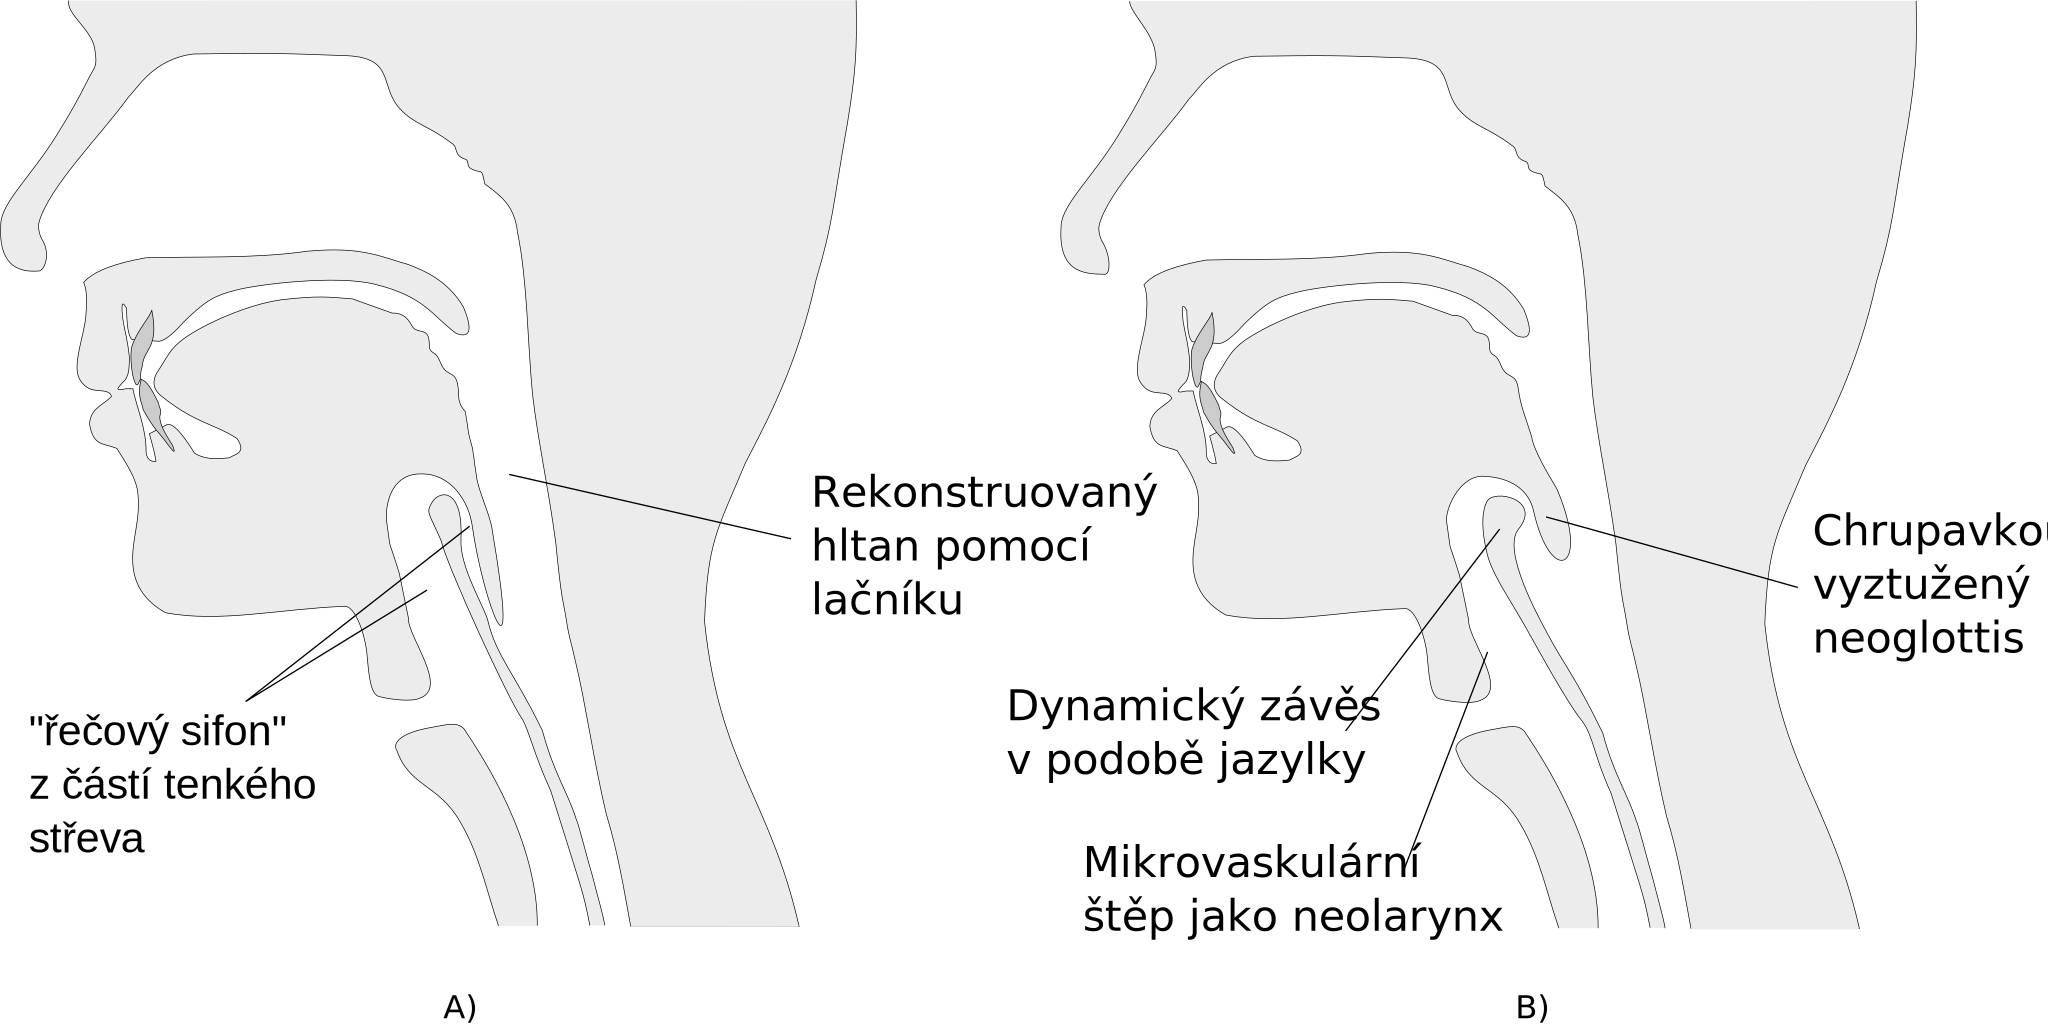
\includegraphics[width=0.9\linewidth]{ch2-cause/figures/microvascular}
    \caption[Schéma \uv{řečového sifónu} a laryngoplastiky]{A) Schéma \uv{řečového sifónu} tak jak jej představil Ehrenberg. B) Laryngoplastika podle Hagena}
    \label{fig:cause:treatment:microvascular}
  \end{center}
\end{figure}

Bohužel v současné době tyto metody nenacházejí širší uplatnění. Především je
to způsobeno chirurgickou náročností samotných metod, kvůli které se velmi
těžko prosazují na dalších pracovištích. Dalším aspektem, který limituje tyto
metody, je vliv na samotného pacienta. Metody předpokládají další chirurgický
zákrok vykonaný po totální laryngektomii. Tento zákrok představuje další zátěž
pro pacienta nemluvě o~možných komplikacích. I přes nedostatky těchto metod je
pochopitelná snaha lékařů o intenzivní výzkum v této oblasti. Při úspěšné
léčbě je pacient schopen produkovat hlas velmi dobré kvality a ve většině
případů nepotřebuje žádnou péči ze strany lékařů ORL.

% subsection hrtanu_podobné_struktury (end)

\subsection{Transplantace hrtanu} % (fold)
\label{sub:cause:treatment:transplantation}

Nejkomplexnější možnost rehabilitace hlasu představuje transplantace hrtanu.
V~tomto případě pacient obdrží implantovaný hrtan od dárce. Pokud je
transplantace úspěšná, přebírá transplantovaný orgán plně funkci původního
orgánu a velmi významně zvyšuje šance pacienta na plné zotavení bez trvalých
následků.

První informace spojené s výzkumem možností provedení transplantace hrtanu se
objevují již v 60. letech 20. století\footnote{Vůbec první úspěšná transplantace
orgánu (ledvin) se uskutečnila v roce 1954.}. Přesto byla první totální
hrtanová transplantace provedena až profesorem Marshallem Stromem v roce 1998
\cite{Narula2011} a do dnešních dnů byly provedeny pouze 2 kompletní
transplantace.

Prvním pacientem, který podstoupil transplantaci, byl čtyřicetiletý muž z USA.
K~laryngektomii v jeho případě vedla motocyklová nehoda, při které si pacient
rozdrtil hrtan. K incidentu došlo 20 let před transplantací. Před zákrokem
používal k~produkci řeči elektrolarynx. Dárcem orgánu byl taktéž čtyřicetiletý
muž, který zemřel na mozkové aneurysma. Úspěch transplantace se na příjemci
projevil již třetí den po operaci, kdy poprvé po 20 letech promluvil (vyslovil
anglické slovo \uv{hello}). Přibližně po 36 měsících od transplantace byl
produkovaný hlas srovnatelný s hlasem zdravého člověka. Podle vlastních slov
pacienta se po operaci jeho kvalita života \uv{nesmírně} zlepšila.
\cite{Strome2001} Doposud poslední úspěšně vykonaná transplantace byla
zaznamenána v~říjnu 2010.

Mezi hlavní důvody takto malého počtu zákroků patří množství pacientů vhodných
pro tuto proceduru. Jelikož se jedná o transplantaci dárcovského orgánu je
nutné použití imunosupresiv, tedy medikamentů zabraňující odmítnutí orgánu.
Imunosupresiva jsou však v současné době nepoužitelná u lidí trpících
rakovinou hrtanu z důvodu velmi vysokého rizika rozšíření rakoviny
\cite{Narula2011}. Další problém představuje náročnost samotného zákroku.
Předně je potřeba provést reinervaci a obnovení krevního oběhu v implantovaném
orgánu. U první provedené transplantace se nepodařilo dosáhnout kompletní
reinervace. Výsledkem tak byl velmi kvalitní generovaný hlas, ale zároveň
nebylo možné pomocí hrtanu zabezpečit bezproblémové dýchání a bylo proto nutné
ponechat tracheostomii.

Poslední výzkum v oblasti imunosuprese však naznačuje, že by v dohledné době
mohlo dojít k pokroku a umožnit transplantaci hrtanu i u lidí trpících
rozsáhlou rakovinou v oblasti krku \cite{Narula2011}. Prozatím je však tato
metoda vhodná pro pacienty netrpící rakovinou, případně ty, u kterých
převažovaly benigní nádory a již 5 let nedošlo k recidivě.

% subsection transplantace_hrtanu (end)

\subsection{Shrnutí} % (fold) \label{sub:treatment:summary}

% NOTE: Neni lepsi pouzit dusledky misto nasledky 3

Rehabilitaci pacientů, kteří prodělali chirurgické odstranění hrtanu, je ve
vyspělých zemích věnována značná pozornost, jelikož následky této operace,
oproti jiným druhům léčby, velmi významně ovlivňují kvalitu života pacientů. V
první řadě se léčený musí vyrovnat se ztrátou hlasu. Tato situace je již sama
o sobě velmi náročnou psychickou zkouškou. Ztráta hlasu je však pouze jedním z
vícero problémů, se kterými je potřeba se vypořádat. Mezi další patří možná
ztráta čichu či vyšší náchylnost k respiračním onemocněním. Neméně významnou
roli sehrává i fyzická odlišnost a z~toho pramenící psychická zátěž pacienta
po absolvované léčbě.

 V současnosti
nejpoužívanějšími metodami rehabilitace hlasu jsou \textbf{tracheoezofageální
píštěl} (popsáno v části \ref{sub:cause:treatment:tracheo}), \textbf{jícnový
hlas} (\ref{ssub:cause:treatment:foniatric:esophageal}) a použití
\textbf{elektrolarynxu} (\ref{ssub:cause:treatment:foniatric:elektrolarynx}).
Existují samozřejmě i další a přehled v současnosti používaných je uveden
v~tab. \ref{tab:treatment:summary}.

\newcolumntype{b}{X}
\newcolumntype{s}{>{\hsize=.5\hsize}X}

\begin{table}[ht]
  \centering
  \begin{tabularx}{1.0\textwidth}{L{1.2} L{0.6} L{1.1} L{1.1}}
    & \textbf{Kvalita} & \textbf{Výhody} & \textbf{Nevýhody} \\
    \toprule \\ [-1.75ex]

    \textbf{Tracheoezofageální píštěl} & Vysoká & Vysoká míra osvojení, dlouhá fonační doba & Zanášení píštěle a s ním spojené čištění, případně dodatečná lékařská péče \\
    \midrule \\ [-1.75ex]

    \textbf{Jícnový hlas} & Dobrá & Volné ruce při mluvení, není potřeba dodatečné lékařské péče & Velmi náročná metoda k naučení, nepřirozený hlas \\
    \midrule \\ [-1.75ex]

    \textbf{Elektrolarynx} & Nízká & Snadné k naučení & Monotonní až robotický hlas, nutné nosit externí elektrické zařízení \\
    \midrule \\ [-1.75ex]

    \textbf{Hrtanu podobné struktury} & Vysoká & Nezávislost pacienta na pravidelné lékařské péči & Velmi náročná chirurgická procedura, která pacienta vystavuje dalším možným rizikům  \\
    \midrule \\ [-1.75ex]

    \textbf{Transplantace hrtanu} & Velmi vysoká & Transplantovaný hrtan přejímá funkci odstraněného orgánu & Velmi náročná chirurgická procedura, která je vhodná jen pro malé procento pacientů \\
  \end{tabularx}

  \caption{Přehled dostupných metod rehabilitace hlasu \label{tab:treatment:summary}}
\end{table}

Většina pacientů je tedy rehabilitována pomocí tracheoezofageálního píštěle,
který principiálně vychází z jícnového hlasu, jehož negativa se snaží
eliminovat. O úspěchu rehabilitace, stejně jako u jícnového hlasu, tak
především rozhodují vlastnosti faryngoezofageálního segmentu. Pokud pacient
není schopen si osvojit jícnový hlas, případně nemá voperován píštěl, je
použit elektrolarynx. Bohužel tyto metody neřeší další problémy spojené s
odstraněním hrtanu, a proto se lékaři stále snaží zdokonalovat rehabilitační
metody. Za nejkomplexnější se dá považovat úplná transplantace hrtanu, která
řeší víceméně všechny problémy spojené s odstraněním hrtanu. Bohužel tento
zákrok je velmi náročný a vhodný pouze pro malou část pacientů.
I když je tedy v současné době lékařská věda schopna rehabilitovat hlas, tak
zde zůstává otevřený prostor pro inovace a tím zlepšení kvality života lidí
postižených ztrátou hrtanu.

% subsection treatment:summary (end)

% section rehabilitace_hlasu_po_totalni_laryngektomii (end)

